%% This file is modified by Veli M�kinen from HY_fysiikka_LuKtemplate.tex authored by Roope Halonen ja Tomi Vainio.
%% Some text is also inherited from engl_malli.tex by Kutvonen, Erki�, M�kel�, Verkamo, Kurhila, and Nyk�nen.


% STEP 1: Choose oneside or twoside
\documentclass[english,twoside,openright]{HYgraduMLDS}
%finnish,swedish

%\usepackage[utf8]{inputenc} % For UTF8 support. Use UTF8 when saving your file.
\usepackage{lmodern} % Font package
\usepackage{textcomp} % Package for special symbols
\usepackage[pdftex]{color, graphicx} % For pdf output and jpg/png graphics
\usepackage[pdftex, plainpages=false]{hyperref} % For hyperlinks and pdf metadata
\usepackage{fancyhdr} % For nicer page headers
\usepackage{tikz} % For making vector graphics (hard to learn but powerful)
\usepackage{svg}
\svgpath{{.}}
\usepackage[ruled,vlined,linesnumbered,noend]{algorithm2e}
%\usepackage{wrapfig} % For nice text-wrapping figures (use at own discretion)
\usepackage{amsmath, amssymb} % For better math
%\usepackage[square]{natbib} % For bibliography
\usepackage[footnotesize,bf]{caption} % For more control over figure captions
\usepackage{blindtext}
\usepackage{titlesec}
\usepackage{listings}
\usepackage[titletoc]{appendix}
\usepackage{booktabs}
\usepackage{courier}

% \DeclarePairedDelimiter{\ceil}{\lceil}{\rceil}
% \DeclarePairedDelimiter{\floor}{\lfloor}{\rfloor}

\onehalfspacing %line spacing
%\singlespacing
%\doublespacing

%\fussy
\sloppy % sloppy and fussy commands can be used to avoid overlong text lines

% STEP 2:
% Set up all the information for the title page and the abstract form.
% Replace parameters with your information.
\title{GPU Accelerated Pseudoalignment}
\author{Daniel Cauchi}
\date{\today}
\prof{Professor Keijo Heljanko}{PhD Jarno Niklas Alanko}
\censors{Professor Keijo Heljanko}{PhD Jarno Niklas Alanko}{}
\keywords{Pseudoalignment, SBWT, Multithreading, GPU, CUDA, HIP}
\depositeplace{}
\additionalinformation{}


\classification{\protect{ \\
        Applied computing $\rightarrow$ Life and medical sciences $\rightarrow$ Computational Biology $\rightarrow$ Computational genomics \\
        Applied computing $\rightarrow$ Life and medical sciences $\rightarrow$ Bioinformatics
}}

% if you want to quote someone special. You can comment this line and there will be nothing on the document.
%\quoting{Bachelor's degrees make pretty good placemats if you get them laminated.}{Jeph Jacques}


% OPTIONAL STEP: Set up properties and metadata for the pdf file that pdfLaTeX makes.
% But you don't really need to do this unless you want to.
\hypersetup{
    bookmarks=true,         % show bookmarks bar first?
    unicode=true,           % to show non-Latin characters in Acrobat’s bookmarks
    pdftoolbar=true,        % show Acrobat’s toolbar?
    pdfmenubar=true,        % show Acrobat’s menu?
    pdffitwindow=false,     % window fit to page when opened
    pdfstartview={FitH},    % fits the width of the page to the window
    pdftitle={},            % title
    pdfauthor={},           % author
    pdfsubject={},          % subject of the document
    pdfcreator={},          % creator of the document
    pdfproducer={pdfLaTeX}, % producer of the document
    pdfkeywords={something} {something else}, % list of keywords for
    pdfnewwindow=true,      % links in new window
    colorlinks=true,        % false: boxed links; true: colored links
    linkcolor=black,        % color of internal links
    citecolor=black,        % color of links to bibliography
    filecolor=magenta,      % color of file links
    urlcolor=cyan           % color of external links
}

\begin{document}

% Generate title page.
\maketitle

\chapter*{Acknowledgements}

Credit where credit is due, I want to thank those people who shared their time with me, those who gave me a chance, and those who offered their services to me in some way or another during the past two years that I have spent pursuing this Master's Programme in Data Science. I will not mention any specific names, not only because they would most likely not fit into a single page, but because I am afraid I would forget someone. Those of you who fulfil the above criteria, you know who you are, and I am eternally grateful to you for cultivating my development and now I hope that I can make you proud with my future achievements.

The research work disclosed in this publication is partially funded by the Endeavour Scholarship Scheme (Malta). Project part-financed by the European Social Fund - Operational Programme II - European Structural and Investment Funds 2014-2020 "Investing in human capital to create more opportunities and promote the well-being of society".

% STEP 3:
% Write your abstract (of course you really do this last).
% You can make several abstract pages (if you want it in different languages),
% but you should also then redefine some of the above parameters in the proper
% language as well, in between the abstract definitions.

\clearpage
\begin{abstract}

Alignment in genomics is the process of finding the positions where DNA strings fit best with one another, that is, where there are the least differences if they were placed side by side.
This process, however, remains very computationally intensive, even with more recent algorithmic advancements in the field.
Pseudoalignment is emerging as a new method over full alignment as an inexpensive alternative, both in terms of memory needed as well as in terms of power consumption.
The process is to instead check for the existence of substrings within the target DNA, and this has been shown to produce good results for a lot of use cases.
New methods for pseudoalignment are still evolving, and the goal of this thesis is to provide an implementation that massively parallelises the current state of the art, Themisto, by using all resources available.
The most intensive parts of the pipeline are put on the GPU.
Meanwhile, the components which run on the CPU are heavily parallelised.
Reading and writing of the files is also done in parallel, so that parallel I/O can also be taken advantage of.
Results on the Mahti supercomputer, using an NVIDIA A100, shows a 10 times end-to-end querying speedup over the best run of Themisto, using half the CPU cores as Themisto, on the dataset used in this thesis.

\end{abstract}

% Place ToC
\mytableofcontents

\mynomenclature

% -----------------------------------------------------------------------------------
% STEP 4: Write the thesis.
% Your actual text starts here. You shouldn't mess with the code above the line except
% to change the parameters. Removing the abstract and ToC commands will mess up stuff.
\chapter{Introduction}

Alignment is the process of finding the best match where one source DNA string matches a target DNA~\cite{Alignment}.
Pseudoalignment is the process of finding out if a substring of the source DNA can be found in the target DNA~\cite{Kallisto}.
The latter has emerged as a faster alternative, which can replace full alignment for a lot of use cases~\cite{Kallisto}.
Kallisto~\cite{Kallisto} was the first tool to introduce pseudoalignment, and after some iterations, Themisto~\cite{Themisto} emerged as state-of-the-art, and more recently Fulgor~\cite{Fulgor} has also shown great promise.
This thesis uses the same method as Themisto, but puts most of the heavy lifting on the GPU.
The implementation is GPU vendor agnostic, so the target GPU may be either from NVIDIA or AMD.
This was achieved with the utilisation of the HIP framework.

The goal of the solution presented prioritises speed, but over that, general usability is given even more importance.
Hence some minor optimisations may have been altered from previous GPU methods~\cite{Harri} as they would have made the tool less usable for users.
This removal of some minor optimisations usually did not significantly affect overall performance, as the pipeline as a whole depends on a lot of hardware features and the benchmarks may vary by a few seconds from one run to the next.
Furthermore, a new feature was added over Themisto which is that invalid DNA base pairs, those containing characters outside of the $ACGT$ alphabet, can be differentiated from the rest of the characters, such that $k$-mers with these characters inside them may be included or ignored individually from $k$-mers which were not found in the de Bruijn Graph.

The approach taken when creating the algorithm was to first divide the pipeline into several components, and then connect the components together.
Next, the full pipeline is benchmarked while recording metrics from each component individually, and then optimise the bottlenecks.
This process was repeated several times.
Using this method and the Mahti supercomputer by CSC, pseudoalignment with an end-to-end throughput of 500MB/s has been observed, which is 10 times faster than Themisto when Themisto would be put on the LUMI supercomputer which has twice the CPU cores.

Some of the components are placed on the CPU.
As a result, these components sometimes became the bottleneck, and were thus also parallelised, using OpenMP.
This makes sure that parallelisation is done on all fronts and using all resources available: the CPU, GPU, as much RAM and VRAM as is available, and as much memory transfer speed available in both ways between CPU and disk as well between GPU and CPU.

Thus, this thesis sets out with the following questions:
(a) Can CPU side implementation be improved through increased parallelisation, so that even with sequences of vastly different sizes, the amount of work between each unit of parallelisation is kept as equal as possible?
(b) Can GPU side implementation be made more usable, specifically by allowing $k \ge 32$ and allowing the differentiation of $k$-mers which are not found in the graph and those which are invalid, without significantly impacting computational performance?
(c) Can the color searching phase of pseudoalignment also be adapted to the GPU such that it may be significantly faster than the CPU version?

The structure of this thesis is as follows.
First, in Chapter~\ref{ch:Background}, the necessary biological, algorithmic, and domain specific background is introduced.
Then, in Chapter~\ref{ch:Methodology}, the contributions of this thesis are presented, through a deep explanation of all the optimisations that have been included to speed up pseudoalignment using the same de Bruijn Graph and Colors structure as Themisto.
The results are then shown in Chapter~\ref{ch:Results}, where the two phases of the proposed method are analysed individually and as a whole.
Lastly, this thesis is concluded in Chapter~\ref{ch:Conclusion} with some thought given as to how this work may evolve alongside ideas for future research.

The first repository produced in this thesis is the FASTA/FASTQ parser which may be found at \url{https://github.com/CowKeyMan/kseqpp_REad}, where version $\mathit{v1.6.0}$ is used.
The pseudoalignment repository may be found at \url{https://github.com/CowKeyMan/SBWT-Search}, where $\mathit{v2.0.0b1}$ is used, and $\mathit{v2.0.0}$ will be released once this thesis is published, and the only difference will be that this thesis will be included in that repository.

\chapter{Background}\label{ch:Background}

This chapter will go through the necessary and interesting genomic biology aspects of the algorithm, for the reader to better understand the implications of the research.
It is meant for readers with little or no biological background, and as such it will start from the basics.
Then, a discussion of algorithms that have come before this thesis is made such that the algorithm introduced and its improvements are put into perspective.

\section{Biology Primer}\label{sec:Biology}

This section will start with an introduction to the natural aspect of biology, including what DNA is and how it can be analysed.
Genomic biology is a wide topic, hence this thesis will stick to what is relevant for it.
Later, this will be linked to how researchers can use sequencing technologies in order to make new inferences.

First is a description of what Deoxyribonucleic Acid (DNA) is.
Each organism is made up of cells, and each cell has different components, but in the center is a nucleus which is the driver of everything else, and within this nucleus is the DNA~\cite{CellBiology}.\@
The actual biology is more complicated than this, however, this is as far as the reader needs to understand about the cell structure.

The DNA contains a sequence of bases: Adenine, Cytosine, Thymine, and Guanine.
For the representation in this thesis, each base is represented by a single character: $ACGT$, corresponding to the first letter of the name of each base.
Each base has a pair, where the bases $A$ and $T$ bind together, and $C$ and $G$ also bind together.
These base pairs then attach to a sugar phosphate backbone to form the double helix of the DNA~\cite{DNA}.
Figure~\ref{fig:DoubleHelix} shows the different parts of the double helix visually.
Note that this representation is usually represented as a twisted ladder, but for clarity, a straightened ladder was chosen for the visualisation.

\begin{figure}[t]
  \centering
  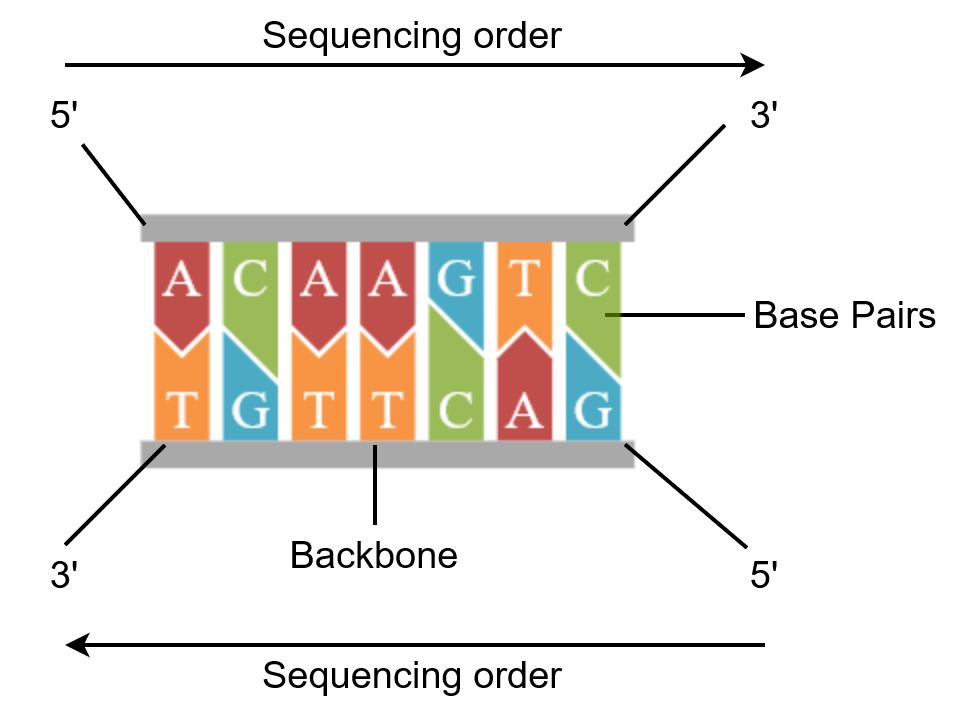
\includegraphics[width=0.55\textwidth]{images/DoubleHelix.png}
  \caption{The double helix of the DNA showing the 2 backbones and the attached base pairs. The visualisation was created using \url{https://www.petercollingridge.co.uk/tools/draw-dna/}}\label{fig:DoubleHelix}
\end{figure}

It is unfortunately very difficult to sequence an entire DNA strand at one go with current technologies.
Instead, a DNA of a sample is cloned multiple times, fractured, and read fragment by fragment~\cite{ShotgunSequencing}.
A sample may have multiple cells from different species, thus having multiple different DNA genomes jumbled together.
Sequencing can either be done using shotgun sequencing~\cite{ShotgunSequencingOriginal}, where each part of the DNA strand has an equal chance of appearing in the dataset, or targeted sequencing~\cite{TargetedSequencing}, where only certain parts of the DNA strand are targeted.
A single fragment is called a read.
The two types of this sequencing are short read sequencing (SRS) and long read sequencing (LRS)~\cite{SrsVsLrs}.
Longer reads are of course preferable because researchers can see more of a genome at a time, whereas with shorter reads, constructing a genome, which is discussed in Section~\ref{sec:DBG}, takes much longer due to the need for assembling many more reads together.
A genome is the full DNA string of a cell of an organism.
However, SRS is currently much more accurate than LRS~\cite{LrsChallenges}.
Accuracy in this case means that the sequenced bases are correct, and an error might be a base-flip, where, for example, an $A$ may be sequenced as a $C$.
Other sources of errors may be missing bases or the addition of non-existent bases.
Cost is also a big factor.
Two big players in these fields are Oxford Nanopore\footnote{\url{https://nanoporetech.com/}}, which perform LRS, and Illumina\footnote{\url{https://www.illumina.com/}}, which perform SRS and were the first to drop the cost of sequencing the full human genome to under \$1000~\cite{LrsChallenges}.
Illumina have been around for almost 20 years now, and have taken a large market share since lots of algorithmic pipelines are based on their technology~\cite{SrsVsLrs}.

To read the DNA, a messenger RNA (mRNA) is used~\cite{mrna} in a method called transcription.
This reads a single strand of the DNA and, luckily, nature has evolved such that the strands are always read from the 5' (five prime) end to the 3' end, as visualised in Figure~\ref{fig:DoubleHelix}.
This means that researchers have more information on the direction of the read, though one still can not know from which of the two strands the read comes from.
A technique that is often used is to also consider the reverse complement of a read.
The reverse complement of a read is the whole string reversed and the bases replaced by their pairs~\cite{ReverseComplements}.
From Figure~\ref{fig:DoubleHelix}, the first strand of the read may be \textit{ACAAGTC}, whereas the reverse complement is \textit{GACTTGT}.\@
Note that both strings may be sequenced with equal probability and it is not possible to know from which strand each string originates from just by looking at the two of them.
One would need to assemble them with other reads in order to know where they belong.

De novo assembly is when different reads are combined together using overlaps in their prefixes and suffixes to construct the full reference genome~\cite{DeNovoAssembly}.
The na\"ive algorithm for this process is to try out all combinations of read pairs and positions and see where they fit best within the context of the whole genome, without knowing what the genome actually looks like~\cite{EulerianPath}.

Ideally, every cell in a body would have the same DNA sequence.
However, mutations do exist, and mutations also develop over time and inevitably lead to aging.
However, many mutations across different parts of the body may lead to severe diseases~\cite{Mutations}.
Hence, analysing these mutations within a genome is one use case for how researchers can use such DNA data and alignment techniques in order to find out more about, for example, the condition of a patient.

To analyse these mutations, alignment can then be used, after a reference genome has been constructed, where the reads of a new specimen are aligned to this genome.
Alignment means to find the best position within the reference genome where there are the least differences between the sequences~\cite{Alignment}.
Gaps may also occur when certain types of mutations occur, and they may also manifest themselves as a character flip within the DNA string.
One use case of alignment could be to find these mutations in the genetic code between healthy people and those with a certain disease, such as forms of cancer~\cite{BreastCancer}.
Figure~\ref{fig:Alignment} shows an example of two aligned reads with some differences.

\begin{figure}[t]
  \centering
  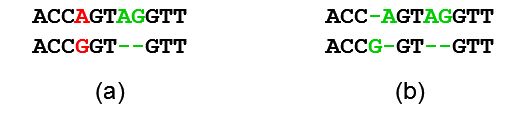
\includegraphics[width=0.55\textwidth]{images/Alignment.png}
  \caption{Two reads aligned to one another. Note that (a) and (b) represent the same two reads, but in one representation the first difference is represented  as a character flip, in red. Meanwhile, in (b) it is represented as 2 separate insertion and deletions in green. Gaps are represented with the '-' character. Since the reference genome is not known in this case, the second difference may be either an insertion or a deletion, or a mixture of both. When doing assembly, these sequences would instead be correlated with more reads to check their correctness and increase the confidence in the accuracy, rather than being compared to the reference genome. If this is all the information that was available, option (a) would be the preferred option to choose as there are fewer operations to align the two sequences.}\label{fig:Alignment}
\end{figure}

Contigs are also explained as they will be a useful concept in Section~\ref{sec:DBG}, mostly unitigs are discussed.
A contig forms when a set of reads is assembled together.
The assembled sequence from end to end is called a contig.
The term \textit{contig} comes from the word \textit{contiguous}, as the reads in the contig set are contiguous~\cite{Contig}.
This contig might contain some uncertainties, due to the mutations described previously.
Figure~\ref{fig:AssemblyAndAlignment} shows a more complex example of alignment with contigs.

\begin{figure}[t]
  \centering
  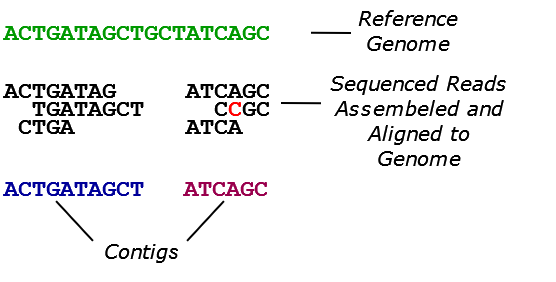
\includegraphics[width=0.55\textwidth]{images/AssemblyAndAlignment.png}
  \caption{A more complex diagram of alignment and assembly. The reference genome is given in green at the top, with the newly sequenced reads, assembled and aligned to the reference genome, in the middle, and the contigs extracted from those reads at the bottom. Note that if the reference genome was not known, then this would be doing De novo assembly, rather than alignment, to try to construct the genome without knowing it.}\label{fig:AssemblyAndAlignment}
\end{figure}

The data is stored in what are known as FASTA and FASTQ files.
An example of the FASTA format may be seen in Figure~\ref{fig:FASTA}.
This format consists of multiple sequences, each starting with the '>' character, followed by the title of the sequence, which is then followed by the sequence itself on the next line.
This sequence can be on multiple lines~\cite{FastaAndFastq}.
Besides the ACGT characters, which are sometimes in uppercase and other times in lowercase, the character N is sometimes used to signal an ambiguous base\footnote{\url{https://knowledge.illumina.com/software/general/software-general-reference_material-list/000003560}}.
The sequences may be genomes or reads.

The second file format is FASTQ, which contains additional information about the quality of each base in the read~\cite{FastaAndFastq}.
An example can be found in Figure~\ref{fig:FASTQ}.
This format starts with the '@' character followed by the title, and the read on the next line which can be of multiple lines similar to the FASTA format.
Then a '+' is added on the next line, which may or may not be followed by the same title of the sequence on the same line, and lastly the quality string on the next line (or lines) which should be of equal length as the sequence.
The characters of the quality string indicate the confidence in the corresponding base at that same index within the sequence.
The specifics of how these characters are interpreted will not be delved into, as they are not relevant to the rest of the text.

FASTA files are usually used for representing reference genomes, while FASTQ files are used for raw read data since they can also contain the quality string.
Unfortunately there is not a single standard for the file formats, although there are some attempts at creating some\footnote{\url{https://www.ncbi.nlm.nih.gov/genbank/fastaformat/}}.
Even the titles themselves can be of any form, as can be seen in the two examples.
The characters used for the quality string are also different between standards.
As such, writing a parser for these file formats can be a headache~\cite{FastaAndFastq}.
For this thesis, a scalable parser capable of supporting both FASTA and FASTQ files, or a mixture of both, was implemented, which is also capable of reading zipped and unzipped files.
This parser skips over title lines and quality strings, since these are not needed for this use case.

\begin{figure}
\centering
\begin{lstlisting}[basicstyle=\footnotesize\ttfamily]
>ERR345345.239 AJIJSDIO
ATCGTCACTAGCTAGCTAGCTACcagagctagtcagctagcactcagtcat
GCTCGAGTCAGC
>seq2
gtagcatcGATCGATCAGTGACNNNNNNNNNNNNNATGTCGAAAGAATAGTCGATG
CGATagtacgctcacgtacgactcgtc
>seq3
GAGTGAGTGCCCCtttaagagtattgtaGT
\end{lstlisting}
\caption{An example of a FASTA file with 3 sequences.}\label{fig:FASTA}
\end{figure}

\begin{figure}
\centering
\begin{lstlisting}[basicstyle=\footnotesize\ttfamily]
@ERR345345.239 AJIJSDIO
ATCGTCACTAGCTAGCTAGCTACcagagctagtcagctagcactcagtcat
GCTCGAGTCAGC
+ERR345345.239 AJIJSDIO
>)II8123))II328947289BA@@@@FFFFDFHFFHGHIGGGBFFAFGCF
;<B;@A5;5<DD
@seq2
gtagcatcGATCGATCAGTGACNNNNNNNNNNNNNATGTCGAAAGAATAGTCGATG
CGATagtacgctcacgtacgactcgtc
+
>)II8123))II328947289BA@@@@FFFFDFHFFHGHIGGGBFFAFGCF3))II
;<B;@A5;5<DD3))II3))II3))II
@seq3
GAGTGAGTGCCCCtttaagagtattgtaGT
+
@@@FFFFDFHFFHGHIGGGBFFAFGCF3))
\end{lstlisting}
\caption{An example of a FASTQ file with 3 sequences.}\label{fig:FASTQ}
\end{figure}

In the next sections, advancements in computer science algorithms will be discussed, which have made the analysis of such data more feasible and accurate.


\section{De Bruijn Graphs}\label{sec:DBG}

The first concept to introduce in this section will be that of the De Bruijn Graph (DBG)~\cite{DeBruijnGraph}, which are used throughout much of bioinformatics.
However, first some notation must be presented.
A graph $G=\{V,E\}$ consists of a set of vertices $V=\{v_1,v_2,\ldots,v_n\}$ which are connected by a set of edges $E=\{e_1, e_2, \ldots, e_m\}$.
The terms nodes and vertex will be used interchangeably.
Each vertex $v_i$ has a label $label(v_i)$, a set of outgoing nodes $out_v(v_i)$ of size $\#out_v(v_i)$, a set of incoming nodes $in_v(v_i)$ of size $\#in_v(v_i)$, a set of outgoing edges $out_e(v_i)$, and a set of incoming edges $in_e(v_i)$, of sizes with the same notation as the vertices.
Then, $v_1$ has an outgoing edge to $v_2$ if there exists an edge $e$ such that $e=v_1 \rightarrow v_2$.
Each edge $e_i$ also has a label $label(e_i)$.

To construct the DBG, the dataset must be transformed.
Given a set of FASTA and FASTQ files, all the sequences must first be extracted individually, and then, using a sliding window method, extract all unique substrings of a set size $k$.
These substrings are called $k$-mers, historically introduced as \textit{k-tuples}~\cite{DeBruijnGraph}.
Formally, given a sequence $S=[c_0, c_1, \ldots, c_{C-1}]$ of size $C$, a set of sequences $\{ [c_0,c_1,\ldots,c_{k - 1}], [c_1, c_2,\ldots,c_{k}], \ldots , [c_{C-k}, c_{C-k+1}, \ldots, c_{C - 1}]\}$ is extracted.
Often, the reverse complements of these $k$-mers are also computed and added to the set of unique $k$-mers.
For this reason, the size of $k$ is usually taken to be an odd number, in order to avoid palindromes between the forward and backwards sequence which can cause problems for some analysis tasks~\cite{Palindromes}.
An example of a palindrome may be \textit{AGCGCT}, where the reverse complement of this sequence would be itself.

Now graph construction may commence.
Given a pair of $k$-mers with sequences $S_0=[a_0, a_1, \ldots, a_{k - 1}]$ and $S_1=[b_0, b_1, \ldots, b_{k - 1}]$, one must first create the nodes $v_0$ and $v_1$ for these $k$-mers and give them the labels $S_0$ and $S_1$ respectively.
Then if the $k-1$ suffix of $S_0$ is equal to the $k-1$ prefix of $S_1$, that is, $[a_1, a_2, \ldots, a_{k - 1}] = [b_0, b_1, \ldots, b_{k-2}]$, create an edge $v_0 \rightarrow v_1$.
The labels of the edges are the character that is added in order to get to the next $k$-mer, that is, the final character of the outgoing node $v_1$, which is $b_{k - 1}$.
This is done for all $k$-mers which share a $k+1$ suffix and prefix.
Figure~\ref{fig:FastaqToDbg} shows an example of the whole pipeline from the FASTA/FASTQ files to a DBG.\@

\begin{figure}[t]
  \centering
  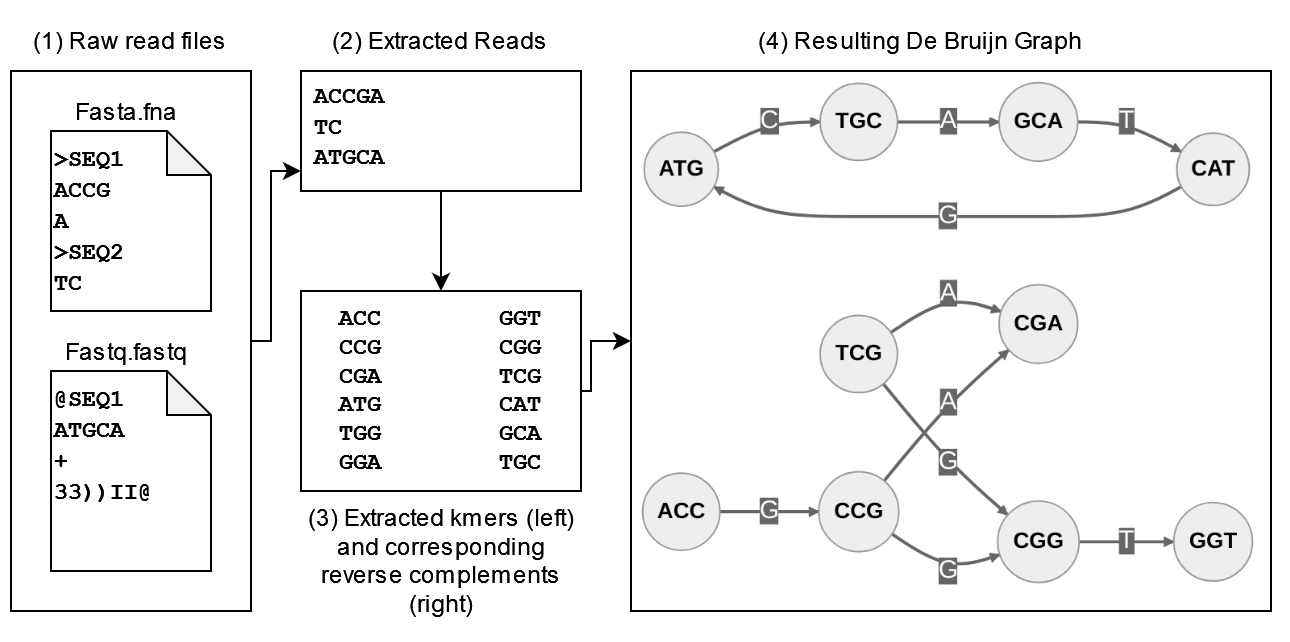
\includegraphics[width=\textwidth]{images/FastaqToDbg.png}
  \caption{The pipeline from FASTA/FASTQ files to the final DBG with $k = 3$.}\label{fig:FastaqToDbg}
\end{figure}

The DBG is a crucial part of many genome analysis tasks.
For example, it can be used to assemble a new genome by traversing it, and if there is a single Eulerian path for the entire graph, then it is known that this is the order in which reads must be assembled~\cite{DeBruijnGraph}.
An Eulerian path is a path that traverses all edges exactly once.
Note that this would not work for the graph in Figure~\ref{fig:FastaqToDbg}, but Figure~\ref{fig:EulerianPath} shows a good example of this.
That said, even this example may not be perfect, because the graph also consists of an unknown number of repeats.
Much work has been done to improve on assembly techniques of new genomes based on this method, especially tackling ambiguity issues when a single Eulerian path might not be possible, such as by giving more weight to certain nodes when they meet certain conditions~\cite{DeBruijnGraph, EulerianPath}.
Some readers may have already started thinking of ways to tackle the many potential challenges of such a problem~\cite{ModernAssembly}, however, this text will not be going into more detail about these assembly methods as they are not relevant to the rest of the contents.

\begin{figure}[t]
  \centering
  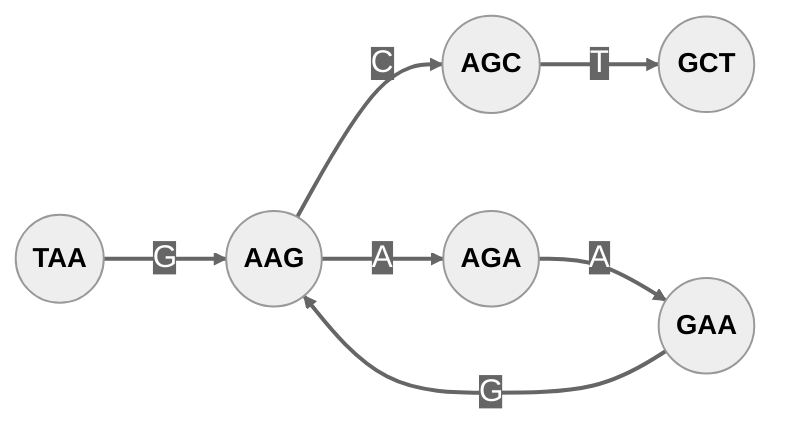
\includegraphics[width=0.6\textwidth]{images/EulerianPath.png}
  \caption{An example of a DBG with $k = 3$ where one can trace a perfect Eulerian path. This path is $TAAGAAGCT$.}\label{fig:EulerianPath}
\end{figure}

From Figure~\ref{fig:EulerianPath}, some properties of its graph can also be pointed out, relating to contigs and unitigs, the former of which was discussed in Section~\ref{sec:Biology}.
For example, the contigs which pass through the nodes $\mathit{TAA} \rightarrow \mathit{AAG} \rightarrow \mathit{AGC} \rightarrow \mathit{GCT}$ can be seen, and the other contig would be the path $\mathit{TAA} \rightarrow \mathit{AAG}$ and $\mathit{AGA} \rightarrow \mathit{GAA}$.
However, none of these are unitigs, because the paths to these contigs branch at the vertex \textit{AAG}.
In this example, one can find the unitig paths $\mathit{TAA}$, $\mathit{AGA} \rightarrow \mathit{GAA}$, $\mathit{AGC} \rightarrow \mathit{AGC}$.
Hence, a unitig is defined as a maximal path with no branching nodes, that is, for all $v_i$ in the path of size $n$, $out_v(v_i) = 1, i = 0,\ldots,n - 2$ and $in_v(v_j) = 1, i = 1,\ldots,n - 1$~\cite{Themisto}.
For the purposes of this text, in Section~\ref{sec:Pseudoalignment}, contigs will not be of use, but unitigs are an important concept and they will further expanded on.

For the SBWT~\cite{SBWT}, which is discussed in Section~\ref{sec:SBWT}, and thus also for this thesis, each node must have at least one incoming node.
To solve this, the nodes without an incoming node, that is, all vertices where $\#in(v_i) = 0$, are taken, and a new node which has the first character a \textit{\$} symbol is added, and the rest of the characters are the first $(k-1)$ characters of the sequence corresponding to the original node.
As an example of these nodes, given a node without any incoming edges corresponding to the $k$-mer $AAT$, one would add a new node $\$AA$.
Recursively, another node is added in the same manner to the new node.
The base case is when the final node which has $k$ $\$$-symbols is added.
Therefore, in the case of the previous example, the nodes $\$\$A$ and $\$\$\$$ are also added.

This means that the alphabet size is now 5: \textit{ACGT} and \textit{\$}.
However, make an important mental note that the nodes never point to another node whose corresponding sequence ends with a $\$$-symbol, that is, no edge will ever contain a $\$$-symbol as a label.
The only sequence which ends with a $\$$-symbol is $\$\$\$$, and this is the only node that does not have any incoming edges.
Thus, it will be seen that there is no need to worry about the expanded alphabet size later on, due to this property.
The altered results from Figure~\ref{fig:FastaqToDbg} are found in Figure~\ref{fig:FastaqToDbgWithDollars}.

\begin{figure}[t]
  \centering
  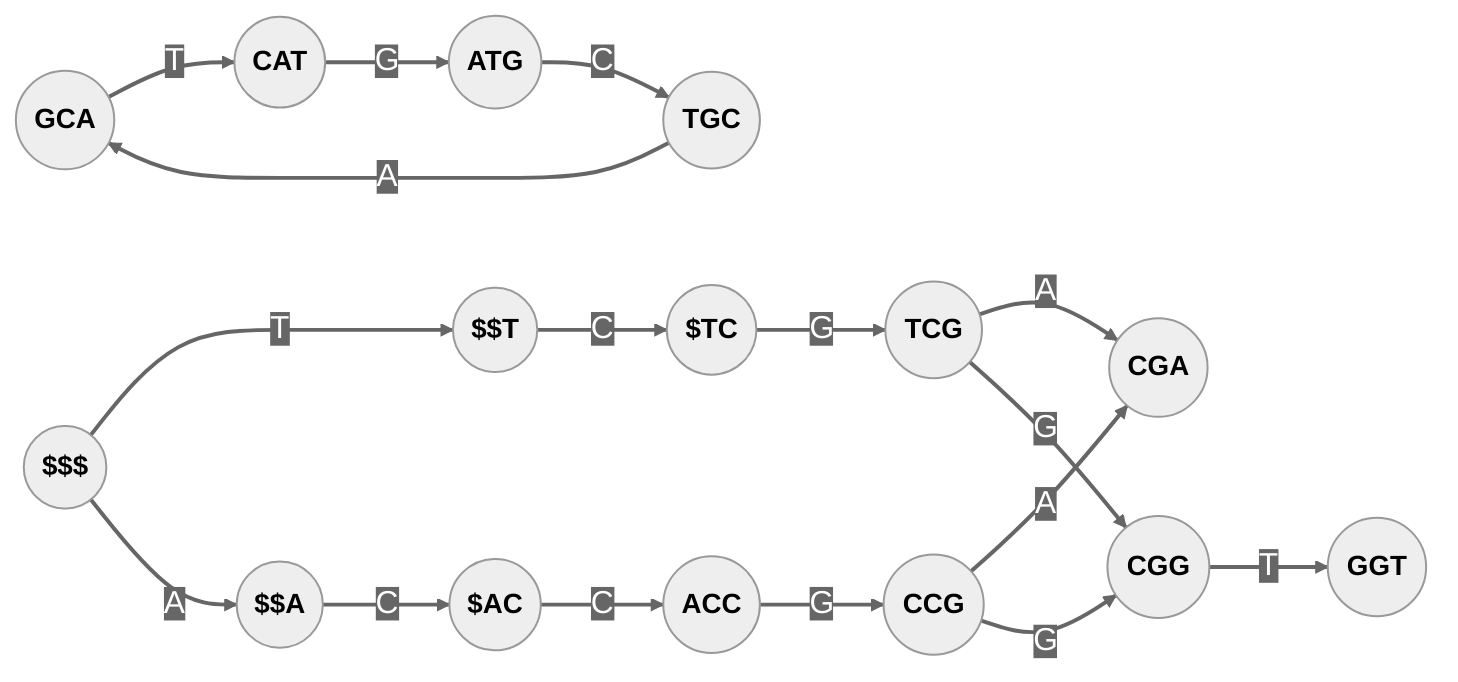
\includegraphics[width=\textwidth]{images/FastaqToDbgWithDollars.png}
  \caption{The altered DBG from Figure~\ref{fig:FastaqToDbg} where extra $\$$ nodes are added to existing nodes with no incoming edges with extra \$-symbols.}\label{fig:FastaqToDbgWithDollars}
\end{figure}


\section{Spectral Burrows Wheeler Transform}\label{sec:SBWT}

Succinct data structures are those which represent the necessary data close to its information-theoretic bound while still allowing fast searches within it~\cite{Succinct}.
The Spectral Burrows Wheeler Transform (SBWT)~\cite{SBWT} represents the DBG as a succinct data structure.
In this case, it represents it as a collection of bit vectors.
The first to do this were the authors of BOSS~\cite{SuccinctDeBruijnGraphs}, but the authors of SBWT managed to create a data structure where searching for the index of a $k$-mer takes $O(k)$~\cite{SBWT}.
In this section, the construction of this structure is discussed, as well as how to use it, and its limitations.
One limitation will be mentioned now to make sure the reader does not get confused while reading.
This data structure only guarantees searches for $k$-mers of fixed size.
This means that if the data structure was built with $k=31$, then it will only support queries for $k$-mers of size $k=31$ or less.

\subsection{Construction}

In this subsection an SBWT structure will be built.
Although the name implies that a Burrows Wheeler Transform (BWT)~\cite{BWT} is used for this succinct data structure, the similarities are distant enough that it is possible to explain the SBWT without going into details of the BWT.\@
Figure~\ref{fig:SbwtConstruction} shows the entire construction pipeline in a single figure, so it is good to refer to it while reading the rest of this section.
The first step is to extract all $k$-mers and reverse complements and create a DBG where an edge $a \rightarrow b$ is drawn for every $k$-mer $a$ and $b$ where the $k-1$ suffix of $a$ is equal to the $k-1$ prefix of $b$.
For example, given $k=3$ and the $k$-mers \textit{ACG, CGA}, and \textit{CGT}, edges $ACG \rightarrow CGA$ and $ACG \rightarrow CGT$ are created, because the $k-1=2$ suffix of \textit{ACG} is equal to the $k-1=2$ prefix of the other two $k$-mers.
The necessary $\$$ $k$-mers are then added to this DBG.\@

Next, the $k$-mers are sorted in ascending colexicographic order.
Colexicographic order means that to get the weight of the string, the reverse of the string must be considered.
After reversing, the  strings can then be sorted in ascending lexicographic/alphabetic order.
The $\$$ character is always weighted as smaller than all the other characters when sorting, meaning that the alphabet, in ascending order, is $\$ACGT$.

From the DBG, the labels of the outgoing edges are extracted and associated with the sorted $k$-mers.
These are then collapsed, such that only the first $k$-mer with a unique suffix of size $k-1$ has outgoing edges.
The collapse is a union, or, since edges with the same $k-1$ suffix will always have the same outgoing edges due to the DBG construction step, one can simply set the outgoing edge label set of the other nodes as the empty set $\emptyset$.
After collapsing, the edge labels column can be replaced with 4 bitvectors, one for each character.
Notice that no edge can ever have a $\$$ symbol, so there is no need for 5 bitvectors, even though the alphabet size is 5.
A cumulative sum map is also created, which is labeled as the c-map.
This stores the cumulative sum of the bit vectors, starting from 1 and then adding up each bit vector for each letter in ascending order.

\begin{figure}[t]
  \centering
  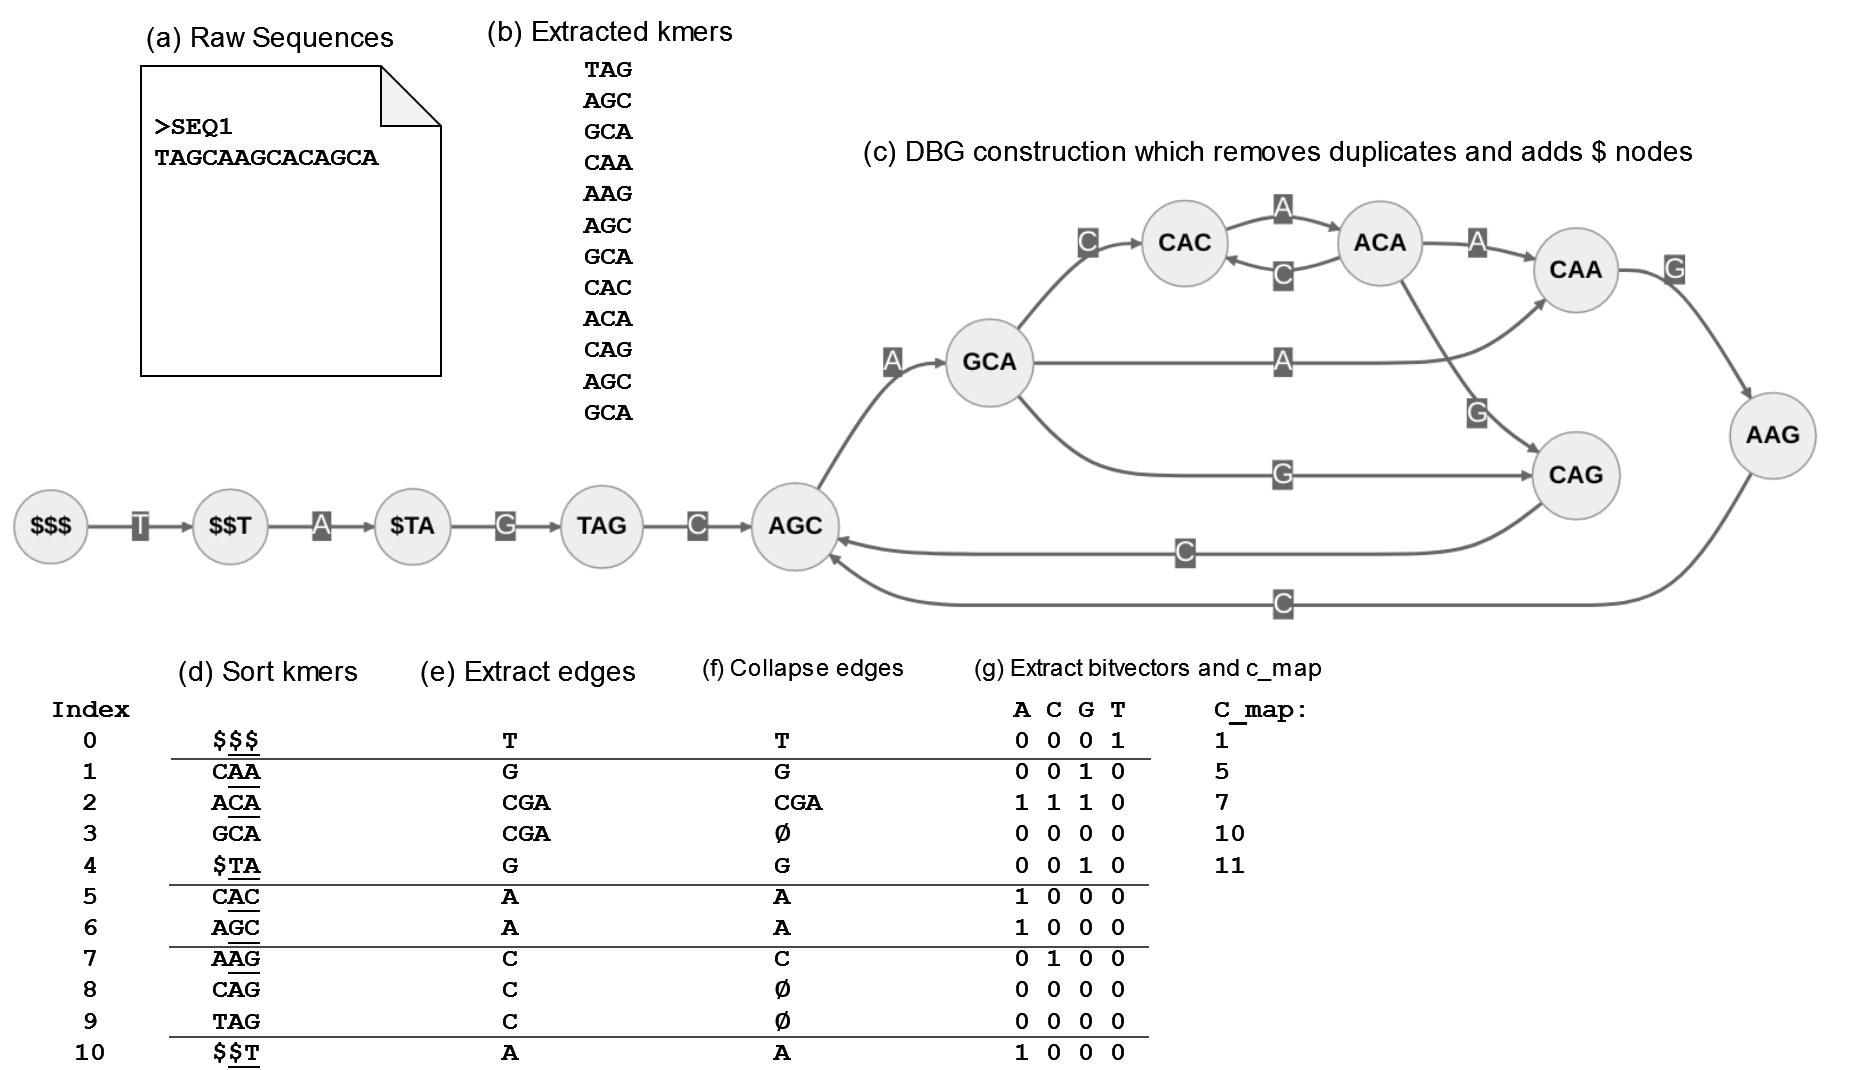
\includegraphics[width=\textwidth]{images/SbwtConstruction.png}
  \caption{SBWT construction pipeline. Note that for this example, the reverse complements are omitted for simplicity and clarity. The first edge is underlined in the sorted lists with unique $k-1$ prefixes.}\label{fig:SbwtConstruction}
\end{figure}

\subsection{Querying}\label{sec:SBWTQuerying}

For querying, one can use a technique similar to a BWT query~\cite{BWT}.
Remember that the only queries which can be done are for $k$-mers of size $k$ or less, that is, the same $k$ used in construction.
The notation will first be defined informally with an informal traversal example, before formally defining the efficient algorithm for traversal.

For the examples, the same construction from Figure~\ref{fig:SbwtConstruction} will be used.
In this figure, long gray lines indicate where the $k$-mers associated with one character begins and where those associated with the previous character ends in the sorted list.
Let $k$-mers associated with a character $c$ mean that the last character of the $k$-mer is $c$.
The list of $k$-mers associated with a character $c$ is $K_c = [k_1, k_2, \ldots, k_{c_{\max}}]$.
To search, two pointers are kept track of, a \textit{left} pointer and a \textit{right} pointer.
In the context of the figure, left means top, and right means bottom.
The algorithm shifts these two pointers around until they meet if the $k$-mers exist, or until the left pointer is greater than the right pointer, in which case it means that the $k$-mer was not found.
These pointers are concerned with the collapsed edges list, so look at these while going through the example.
The informal pseudo code is given in Algorithm~\ref{alg:IndexSearchInformalPseudoCode}, and the formal pseudo code will be discussed next and is then summarised by Algorithm~\ref{alg:IndexSearchFormalPseudoCode}.

\begin{algorithm}
	\KwIn{\newline
    A sequence $S = c_1, c_2, \ldots, c_k$ \newline
    The list of collapsed edges \newline
		The list of indexes where each $k$-mer set associated with one character starts and ends\newline
	}
	$\mathit{left}$ = index of first $k$-mer associated with $c_1$

	$\mathit{right}$ = index of last $k$-mer associated with $c_1$

	\ForEach{c \textbf{in} S[2 \ldots $k$]}{
    $\mathit{left}$ = index of first $k$-mer associated with $c$ + number of characters $c$ up to this pointer in the collapsed edges list ($\mathit{left}$), the index of this pointer not included

    $\mathit{right}$ = index of first $k$-mer associated with $c$ + number of characters $c$ up to this pointer in the collapsed edges list ($\mathit{right}$), the index of this pointer included \-- 1

    \If{$\mathit{left}$ > $\mathit{right}$}{\
      \textbf{return} not found
    }
  }
  \textbf{return} $\mathit{left}$ \textit{// or }$\mathit{right}$\textit{, they will have the same value}
	\caption{Index Search function (Informally Defined)}\label{alg:IndexSearchInformalPseudoCode}
\end{algorithm}

This next part will go through a full example search for the sequence $\mathit{CAC}$, which is know to exist in the dataset.
While doing this example, the reader is invited to look at Figure~\ref{fig:IndexQueryExample} for a visual representation of the movement of the left and right pointers.
The first character is $C$, so the algorithm starts by placing the pointers at the start and end of the $k$-mers associated with the character $C$, that is, indexes 5 and 6 for the left and right pointers respectively.
The next character is $A$, so the algorithm performs a check for how many $A$s there are in the collapsed edges list, until it gets to each of the left and right pointers, with the exception that for the left pointer, the $A$ at the index of this pointer itself is not included.
Thus, for the left pointer, the algorithm has a single $A$, so it moves the left pointer to the index of the $k$-mer associated with the first $A$ + 1, that is, index 2.
At index 6, including the index itself, it has three $A$s, so it moves this pointer to the index of the $k$-mer associated with the first $A$ + 3, that is, index 3.
Lastly, the right pointer must be moved one index downwards, so now it is at index 2, same as the left pointer.

\begin{figure}[t]
  \centering
  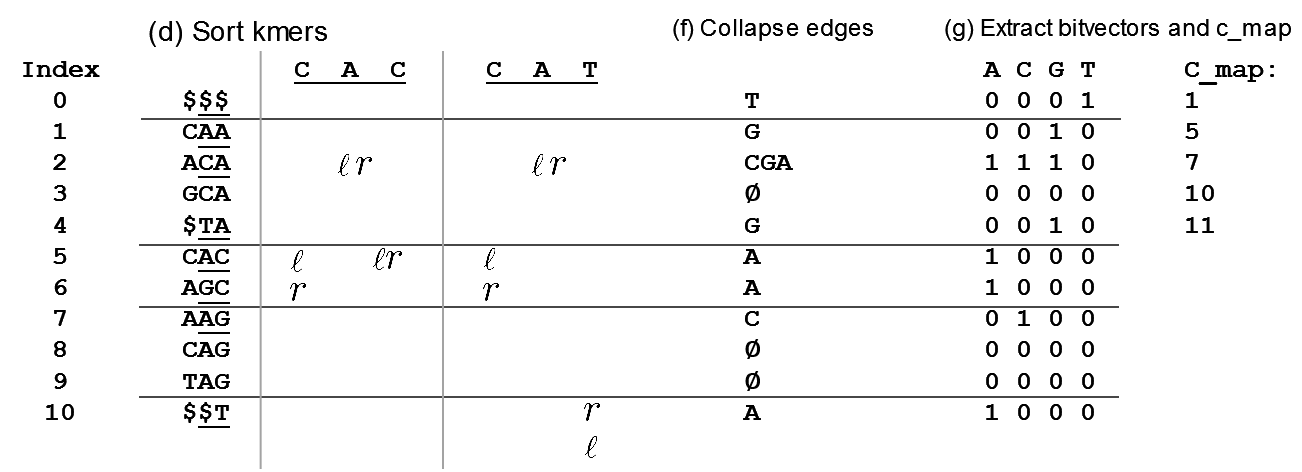
\includegraphics[width=\textwidth]{images/IndexQueryExample.png}
  \caption{Two examples of querying through the SBWT structure created in Figure~\ref{fig:SbwtConstruction}. The sequences $CAC$ is searched, which is found, and $CAT$ is not found.}\label{fig:IndexQueryExample}
\end{figure}

Lastly is the character $C$ again.
At the left pointer, up to this point there have been no $C$s in the collapsed edge list, so the pointer is moved to the index of the $k$-mer associated with the first $C$, that is, index 5.
Including the index at the right pointer, a single $C$ has been seen, so the pointer is moved to the index of the first $C$ + 1, to index 6, and then move one index backwards, to index 5.
The algorithm has now reached the end of the string, and the left and right pointer are equal and are both at index 5, which means that the index of the $k$-mer $CAC$ in the SBWT is 5.
By looking at the sorted $k$-mer list again, this claim may be verified.
The reader is encouraged to try this with other $k$-mers as well.

In the end of a $k$-mer query, the left and right pointer will always be equal, if the $k$-mer has been found.
This works because the $k$-mers are sorted and the edges are collapsed.
When the edges are collapsed, the algorithm is essentially making sure that in the DBG, each edge only has a single incoming node~\cite{SBWT}, as seen in Figure~\ref{fig:PrunedDBG}.
Next is an example using the same technique, but for a $k$-mer not present in the dataset.

\begin{figure}[t]
  \centering
  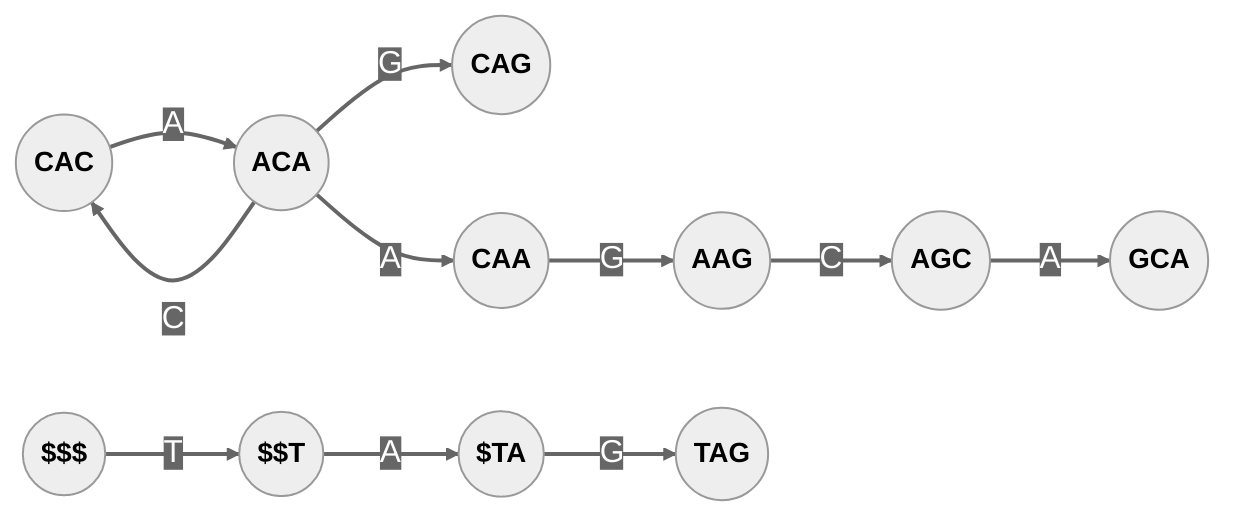
\includegraphics[width=\textwidth]{images/PrunedDbg.png}
  \caption{Pruned DBG from figure~\ref{fig:SbwtConstruction}}\label{fig:PrunedDBG}
\end{figure}

Now the sequence $\mathit{CAT}$ is considered.
Following from the previous example, both of the pointers will be at index 2 after considering both characters C and A.
Now put the left pointer at the index associated with the first $T$ + the number of $T$s seen thus far, which is $10 + 1 = 11$.
Similarly, the right pointer is put in the same location \-- 1, that is, at index 10.
Now, the left pointer is greater than the right pointer, so the algorithm will return that the $k$-mer has not been found.
Figure~\ref{fig:IndexQueryExample} also shows this example visually.

Now comes the definition for how one can do these queries algorithmically and in an efficient manner.
Notice that by using the c-map, one can know where the first $k$-mer associated with each character is.
The first element of this map is always 1, due to the node containing $k$ $\$$s.
Then, using the bitvectors for each character, the number of characters that exist up to that point in the collapsed edge list can be known, by counting the number of 1s.
To count the number of 1s, the algorithm uses what is known as the rank function for bitvectors.
Thus, $rank(b, i)$ gives the number of 1s for the bitvector $b$  up to but not including the index $i$.
For example, given $b=010110$ in binary, $rank(b, 0) = 0, rank(b, 1) = 0, rank(b, 2) = 1, rank(b, 3) = 1, rank(b, 4) = 2, rank(b, 5) = 3$ and $rank(b, 6) = 3$.
The formal definition of the algorithm can be now seen in Algorithm~\ref{alg:IndexSearchFormalPseudoCode}.

\begin{algorithm}
	\KwIn{\newline
    A sequence $S = c_1, c_2, \ldots, c_k$ \newline
    Bitvectors $b_A, b_C, b_G, b_T$
    c-map $C$
	}
  $\mathit{left}$ = $C[c]$

  $right$ = $C[c+1]$\--1  \textit{// C[A] = C[0], C[C] = C[1], \ldots}

	\ForEach{c \textbf{in} S[2 \ldots $k$]}{
    $\mathit{left}$ = $C[c]$ + rank ($b_c$, $\mathit{left}$)

    $right$ = $C[c]$ + rank ($b_c$, $\mathit{right} + 1$) \-- 1

    \If{$\mathit{left}$ > $\mathit{right}$} {\
      \textbf{return} not found
    }
  }
  \textbf{return} $\mathit{left}$
  \caption{Index Search function (Formally Defined)}\label{alg:IndexSearchFormalPseudoCode}
\end{algorithm}

Note that since $i$ itself is not included, $\mathit{rank}(0) = 0$ always holds.
Some other material may define this rank function a bit differently, such as including the 1s at index $i$, however, in this thesis, it is defined this way in order to stay true to the implementation.
This is also the implementation used by $sdsl$~\cite{SDSL}, which is a popular bitvector manipulation library.
Knowing all this, one can view the c-map as a cache for cumulative bitvector sums (+1), which means that when storing the SBWT, only two items are needed: the bitvectors, and the value for $k$, as everything else can be recomputed.

The heaviest part of this algorithm is the rank function.
Counting the number of 1s from the start of the bitvector at each step would be extremely inefficient.
On the previous CPU implementation of Themisto~\cite{Themisto}, the SDSL~\cite{SDSL} rank function is used.
Meanwhile, on the previous GPU implementation~\cite{Harri}, the Poppy data structure~\cite{Poppy} is used, to turn the rank function from $O(n)$, where $n$ is the number of vertices in the DBG, to $O(1)$, needing at most 3 cache line accesses per query.
This makes the entire search function $O(k)$.
For this thesis, Poppy is used, hence this will be further focused on.
Another advantage of this data structure is that its memory footprint is negligible, as it only uses 6.25\% more memory than the bitvector alone~\cite{Poppy}.

To construct the Poppy data structure, the vectors can be scanned once and checkpoints are inserted at each step.
For those familiar with skip lists, the cost-saving ideas are comparable.
Checkpoints are set at 3 layers.
Layer 0 stores a checkpoint every $2^{32}$ bits, so that it counts the total cumulative number of bits.
This type of cumulativeness is called absolute cumulative.
Thus, $2^{32}$ is the hyperblock size.
Layer 0 is stored as a bitvector of 64-bit integers.

Next is to construct layer 1.
This layer is similar to to layer 0 but it stores a checkpoint after $2^{10} = 1024$ bits.
$2^{10}$ is the superblock size.
Another special feature of this layer is that it resets to 0 once it reaches one of the layer 0 checkpoints, that is, once the number of bits it has covered reaches the hyperblock size, it restarts from 0.
This gives it the feature that layer 1 counts will always have a maximum size of $2^{32}$, and thus can be stored in 32-bit integers.

Lastly is layer 2, which sets a checkpoint after every $2^8 = 256$ bits, or after every $4 \times 64$ bits.
$2^8$ is the basicblock size.
This layer is not cumulative at all, unlike the previous two layers, where layer 1 is relative cumulative and layer 0 is absolute cumulative.
The maximum value for layer 2 is $2^8$, which means that for each value, they only need 8 bits.
Layer 3 could be considered to be the bitvector itself.
The full data structure is shown in the first part of Figure~\ref{fig:Poppy}.

\begin{figure}[t]
  \centering
  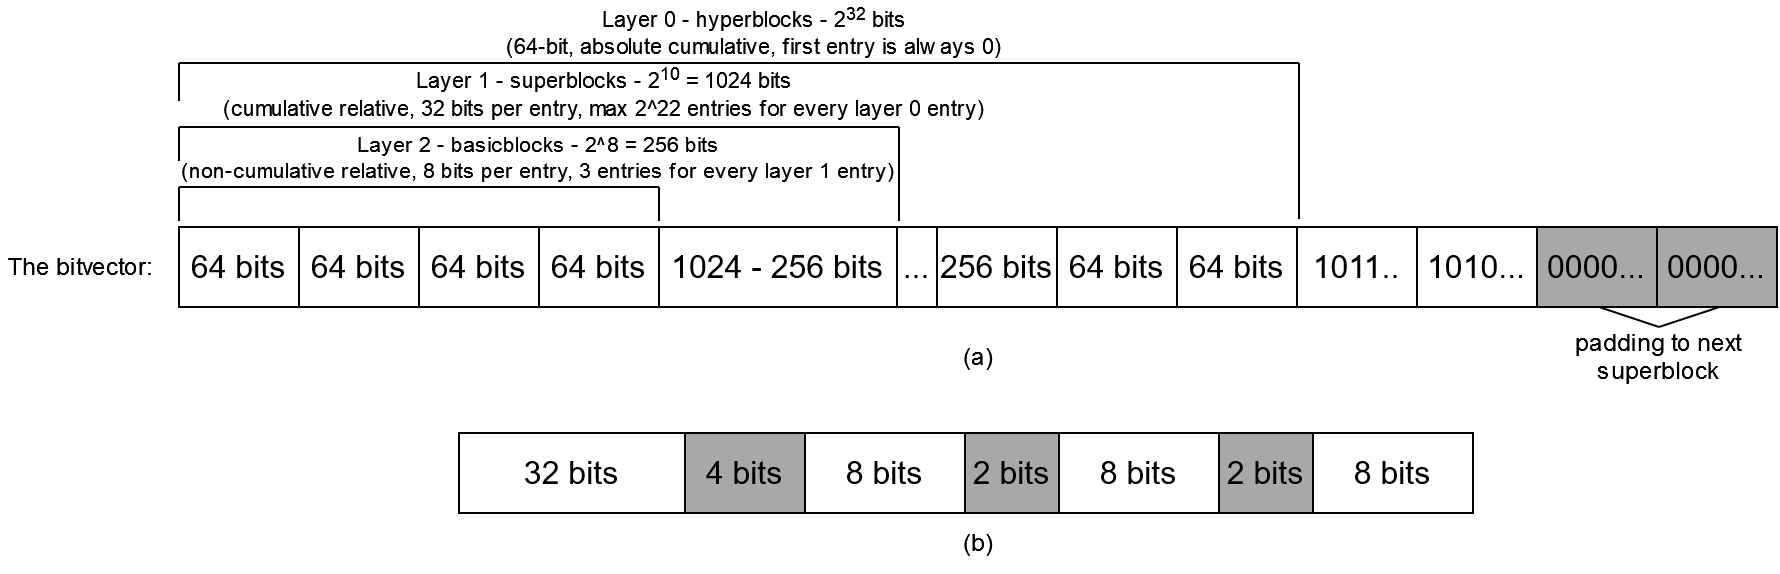
\includegraphics[width=\textwidth]{images/Poppy.png}
  \caption{(a) Poppy data structure fully constructed, with padding shown to the next superblock. (b) The combined storage representation for layer 1 and layer 2.}\label{fig:Poppy}
\end{figure}

Then, to query, one would need to first obtain the previous layer 0 entry, which always has a 0 entry at the start for convenience.
This entry is then added to the previous layer 1 entry, which also has a 0 entry at the start.
The result would then need be added to the previous layer 2 entries within the same superblock.
Lastly, the rank of the integers within the same basicblock is added up until the index needed for the rank function.

The storage of layers 1 and 2 can be combined in a single 64-bit integer, so the data structure can have a layer 1 entry and the inner layer 2 entries.
This is shown in the second part of Figure~\ref{fig:Poppy}.
As a result of this optimisation, the algorithm may need to do more bit shifting in order to obtain the values for layers 1 and 2, however the values in these layers can be accessed with a single memory access, which is usually a bigger bottleneck than bit shifts.
The big advantage of this data structure is that it can handle vectors up to $2^{64}$ bits, which is the maximum that the algorithm as a whole can handle.

This concludes the SBWT section.
Note, again, that this algorithm guaranteed to find $k$-mers of the size of the same $k$ with which the algorithm was built for, or less.
As such, $k$ should be as large as possible, if accuracy is the goal.
However, the larger the $k$, the larger the memory footprint of the index, so it is not recommended to go overboard.
$k=31$ is a usual choice, as the entire query can fit into a single 64-bit integer by bit packing ACGT into 2 bits each, though this technique is not used by the implementation for this thesis, which is in Section~\ref{sec:Phase1}.
$k$ is taken to be 31 since this is an odd number and palindromes should be avoided, as discussed earlier.
The disadvantage of this data structure is that information is lost as to where the $k$-mer originated from, if the input consists of multiple reads, or multiple files.
The next section will describe how additional labels, known as colors in this domain, can be added to the vertices in the DBG in order to determine where the $k$-mers originate from.


\section{Pseudoalignment}\label{sec:Pseudoalignment}

\subsection{Background}

To start describing pseudoalignment, colored DBG must be described first~\cite{CDBG, SuccinctColoredDeBruijnGraphs}.
Throughout this chapter and beyond, the terms $u64$, $u8$, and other variants may be used.
$u64$ means an unsigned 64-bit integer, whereas $u8$ means an unsigned 8-bit integer, and so on for other values of this format.
Lets take a look at Figure~\ref{fig:FastaqToCdbg}.
Say that you are given 2 sequences $S_1$ and $S_2$ with $k$-mer sets $K_1 = a_1, a_2, \ldots, a_n$ and $K_2 = b_1, b_2, \ldots, b_m$.
Now each sequence is given a label, usually some u64.
If a $k$-mer belongs to a sequence, the $k$-mer is marked with the same label as the sequence.
Moreover, if a $k$-mer belongs to multiple sequences, it is marked with the label of that sequence.
These labels are the colors.
Implementation-wise, these colors are represented as simple u64s, so each $k$-mer has a set of u64s associated with it~\cite{Themisto}.

\begin{figure}[t]
  \centering
  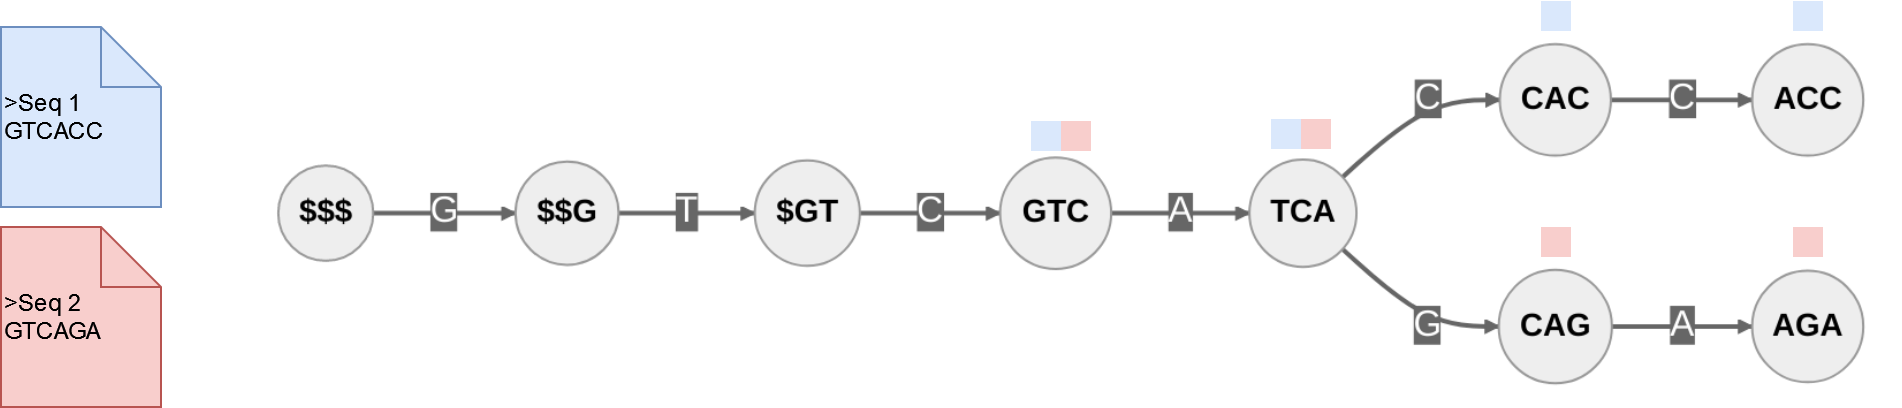
\includegraphics[width=\textwidth]{images/FastaqToCdbg.png}
  \caption{Transforming FASTA/FASTQ files into a colored DBG with $k=3$. Reverse complements are not included in this example.}\label{fig:FastaqToCdbg}
\end{figure}

Different sequences may have the same color.
One use of this is to group the sequences of a single reference genome and say they all have the same color.
This way, if a $k$-mer is labeled with the color of a reference genome, it is known that the $k$-mer is found in that genome.
Then, if all the color sets of all $k$-mers of a read contain the same color, that is, the intersection of all the color sets has a color, one may say that the read is found in the reference genome associated with that color.
If a $k$-mer is not found in the DBG, then it is ignored.
This is the technique used by Kallisto~\cite{Kallisto}, the first pseudoalignment tool.

Metagraph~\cite{Metagraph} and Bifrost~\cite{Bifrost}, two separate pseudoalignment tools, went one step further than Kallisto and instead of ignoring the $k$-mers not found in the DBG, they set a threshold $\tau$, and if more than $\tau$ color sets of $k$-mers in a read include a color, then it is said that the read is associated with that color.
Themisto~\cite{Themisto}, whose implementation this work is based on, combines the two methods so that the user can choose to remove or include the $k$-mers with no color sets, and then set a threshold on the remaining $k$-mers.
If a threshold $\tau=1$ is set and the missing $k$-mers are ignored, then the result is the same as Kallisto.
Meanwhile, if the missing $k$-mers are included, the results are the same as those of Metagraph and Bifrost~\cite{Themisto}.
Themisto has shown to be the best method as, besides supporting both threshold and the removal of missing $k$-mers, it is usually faster and uses less space than other methods~\cite{Themisto}.
Metagraph has the potential of using less memory for its index when using binary-relation wavelet trees, but then has 100 times less query throughput on some datasets~\cite{Themisto}.

When doing pseudoalignment, a DBG is usually built out of the $k$-mers of many reference genomes, and each $k$-mer is given the colors of all genomes it belongs to.
Thus, there are as many colors as genomes within this DBG.
However, if the dataset has hundreds of thousands of genomes, it may be a good idea to group some of them together, thus avoiding having too many colors, as this may lead to intense memory requirements and processing times, especially if each $k$-mer has its own color set.
Pseudoalignment works because it was found that it is often not necessary to know in which position a read was within a genome to attribute it to a genome, only which genome it originated from~\cite{Kallisto}.

\subsection{Themisto}

Now, the construction and optimisations of the colored DBG as used in Themisto~\cite{Themisto}, which uses GGCAT~\cite{GGCAT} for colored unitig construction, will be discussed.
Firstly, there is no need to keep a color set for every $k$-mer.
Rather, certain conditions can be identified where the $k$-mers must have an associated color set, and for the rest of the $k$-mers the algorithm would need to move forward in the graph until the next $k$-mer which has a color set.
If two $k$-mers have the same color set, they can point to the same memory position, rather than duplicating the colors, hence avoiding doubling memory requirements.
The $k$-mers with a color set associated with them are called key-$k$-mers.
The conditions for a vertex to be labeled as a key-$k$-mer, and therefore must have a color set associated with it, are described next, and visualised in Figure~\ref{fig:KeyKmers}.
Reference is made to this figure as each condition is described.

The first condition out of four for being a key-$k$-mer is if it is outgoing to another vertex which is the first $k$-mer from a reference sequence.
This condition causes the vertex with $k$-mer \textit{CTT} to be a key-$k$-mer.
The second condition is if it is the last $k$-mer of a reference sequence.
This condition causes $k$-mers \textit{CCT, CGG} and \textit{GAG} to be key-$k$-mers.
Third, if it has an outgoing edge to a vertex $v_i$ with $\#in_v(v_i) \ge 2$.
Because of this, \textit{TAC} and \textit{AAC} are labeled as key-$k$-mers.
Fourth and last, if the vertex $v_i$ itself has $\#out_v(v_i) \ge 2$.
The last condition causes \textit{TCG} to be labeled as a key-$k$-mer.
Notice how each unitig will have the same color set, unless a new sequence starts in the middle of that unitig.

Remember that these rules exist because one can always go forwards in the graph, using Algorithm~\ref{alg:MovingForward}, but not backwards.
This algorithm assumes a single outgoing edge from the current vertex, otherwise, it would lead to ambiguities.
The less steps needed, the better, because for each step in the graph walk that needs to happen requires a random read, since the $k$-mers are not ordered by their position in the graph, but colexicographically based on their $k$-mers.
As a result, ideally, every vertex would be a key-$k$-mer, which means that the color set for each $k$-mer would be stored.
However this causes too much memory to be used, as it would be necessary to store a pointer for each $k$-mer.
Hence why checkpointing is used, with a parameter $d$, where every d $k$-mers of a uniquely colored unitig becomes a key-$k$-mer.
If $d=1$, this means that every $k$-mer is a key-$k$-mer.
In Chapter~\ref{ch:Results}, the datasets used for this thesis are evaluated with $d=1$ and $d=20$.

\begin{figure}[t]
  \centering
  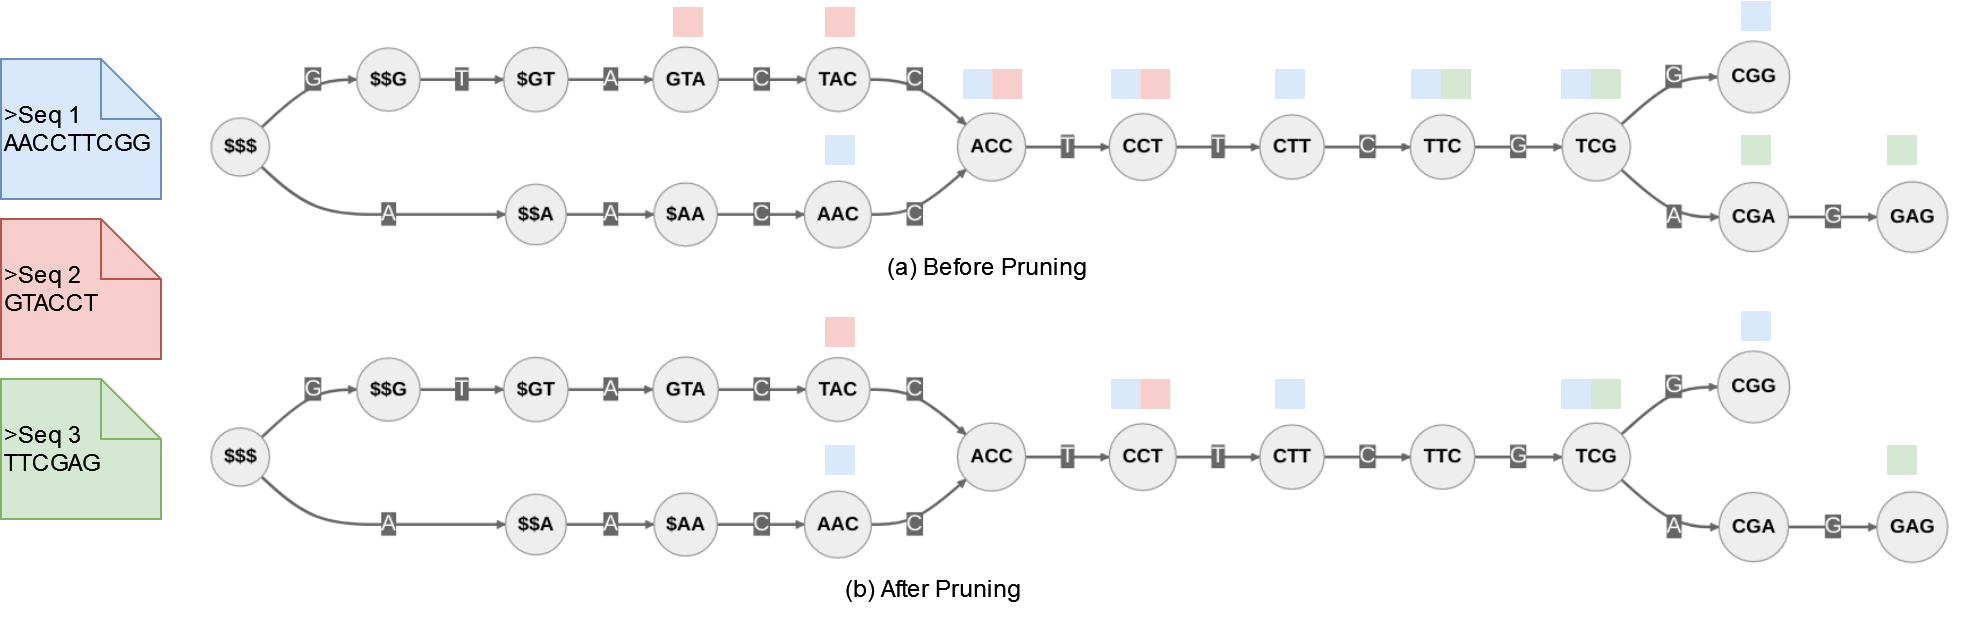
\includegraphics[width=\textwidth]{images/KeyKmers.png}
  \caption{Transforming FASTA/FASTQ files into a colored DBG with $k=3$ and then pruning it for key-$k$-mers. Once more reverse complements are omitted for simplicity of the example, but these would be included also in practice.}\label{fig:KeyKmers}
\end{figure}

\begin{algorithm}
	\KwIn{ \newline
    The current index $i$ \newline
    Bitvectors $b_A, b_C, b_G, b_T$ \newline
    c-map $C$
	}

  \ForEach{$b, label$ \textbf{in} $Bitvectors, BitvectorLabels$}{\
    \If{$b[i]$ = 1}{\
      \textbf{return} $C[label]$ + rank($b_{label}, i$)
    }
  }
	\caption{Walking 1 step forward in the SBWT}\label{alg:MovingForward}
\end{algorithm}

Next the color set storage in Themisto is discussed.
Figure~\ref{fig:ColorComponents} contains a visualisation of each of the components which makes up the whole color structure.
First is a bitvector indicating the key-$k$-mers, the \textit{key\_kmer\_marks}, where a 1 at index $i$ indicates that the vertex at index $i$ corresponds to a key-$k$-mer.
The length of this bitvector is the same length as the number of vertices.
Next, there is the color set indexes \textit{color\_set\_idxs}, which are integers that point key-$k$-mers to the index of the color set they are associated with.
Additionally, a bitvector of the same size of the \textit{key\_kmer\_marks} indicates how the color set for that $k$-mer is stored, the \textit{is\_dense\_marks}.

Themisto uses an adaptive color set storage method which allows it to save a lot of space, which is called the \textit{hybrid} technique.
Using this method, there are two ways a color set can be stored: dense or sparse.
The dense method stores color sets as bitvectors, where a 1 indicates that the color at that index is present.
Any trailing 0s are truncated as an optimisation.
The bitvectors for the dense color sets are stored contiguously in a large bitvector called the \textit{dense\_arrays}.
Thus, another vector of unsigned integers is necessary, to indicate at which bit each color set starts and ends, called the \textit{dense\_arrays\_intervals}.
This array has a final unsigned integer at the end that has the end of the last vector, which would be the start of the next bitvector if it existed.
A compact vector of unsigned integers is used.
Compact means that the vector uses only as much memory as needed, by using $\lceil log_2(n) \rceil$ bits per character, where $n$ is the largest index.
The sparse format then uses compact vectors to store the color set indexes which are present in a color set, the \textit{sparse\_arrays}.
Similarly to the dense format, the sparse vector is stored contiguously, so another compact vector is used to store the start indexes, dubbed as the \textit{sparse\_arrays\_intervals}.
Each sub-array in the \textit{sparse\_arrays} is sorted, to make querying and therefore intersecting the color sets of reads later easier.

\begin{figure}[t]
  \centering
  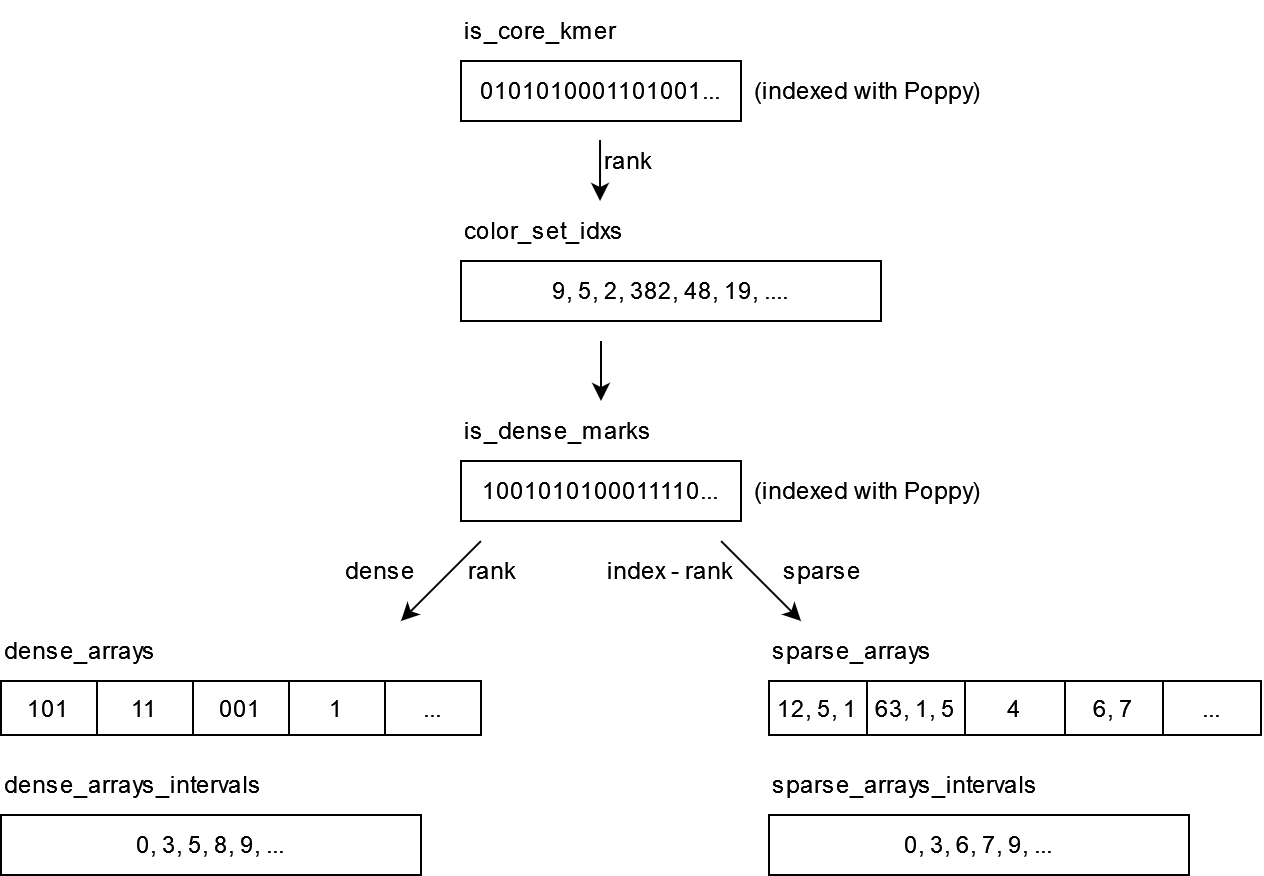
\includegraphics[width=0.85\textwidth]{images/ColorComponents.png}
  \caption{A visualisations of all components used for color storage and some hints for searching. Note that all non-bitvector arrays are compact unsigned integer vectors.}\label{fig:ColorComponents}
\end{figure}

Algorithm~\ref{alg:ColorSearch} shows the color set search, given the index of a key-$k$-mer.
This corresponds to Figure~\ref{fig:ColorComponents} and the terminology used so far, which will carry on to the next section as well.
Themisto uses some optimisations for combining color sets.
For example, when $\tau=1$, a technique which is also used in Kallisto~\cite{Kallisto}, is that when both color sets that need to be combined are dense, a bitwise AND can be used.

\begin{algorithm}
	\KwIn{ \\
    The index $i$ of a key-$k$-mer in the SBWT structure

    $key\_kmer\_marks$ (indexed with Poppy)

    $color\_set\_idxs$

    $is\_dense\_marks$ (indexed with Poppy)

    $dense\_arrays$

    $dense\_arrays\_intervals$

    $sparse\_arrays$

    $sparse\_arrays\_intervals$

    $num\_colors$
	}

  $color\_set\_idx$ = $color\_set\_idxs[rank(key\_kmer\_marks, i)]$

  $is\_dense$ = $is\_dense\_marks[color\_set\_idx]$

  $is\_dense\_rank$ = rank($is\_dense\_marks, is\_dense$)

  \If{is\_dense}{\
    $start$ = $dense\_arrays\_intervals[is\_dense\_rank]$

    $end$ = $dense\_arrays\_intervals[is\_dense\_rank$ + 1]

    \textbf{return} $dense\_arrays[start, \ldots, (end - 1)]$  // returns dense format
  }\Else{
    $start$ = $sparse\_arrays\_intervals[is\_dense\_rank]$

    $end$ = $sparse\_arrays\_intervals[is\_dense\_rank + 1]$

    \textbf{return} $sparse\_arrays[start, \ldots, (end - 1)]$  // returns sparse format
  }

	\caption{Obtaining the color set given the SBWT index and the color structure components.}\label{alg:ColorSearch}
\end{algorithm}

This concludes the background chapter.
The next chapter will discuss the contributions of this thesis to massively parallelise and use all computing resources available to speed up pseudoalignment.


\chapter{Methodology}\label{ch:Methodology}

The final algorithm is split into two phases.
In the first phase, dubbed as the \textit{index search}, given sequences from multiple FASTA/FASTQ files, searches for the key-$k$-mers.
Then, this index is written to disk, and in the second phase it is read again, where the second phase is known as the \textit{color search}.
In this section, the pipeline of both phases are described first.
The two phases bear a lot of similarities, hence these are further expanded upon in the description of the first phase and some of them will be mentioned again without going into detail when describing the second phase.
Later, some additional techniques will be described, which are used in order to massively parallelise and optimise the phases, which are also common between the two of them, but can be described separately from the main pipeline.
With this structure, the reader will get a good idea of how the data flows and also gets familiar with the components, before jumping into more complex optimisations which would be difficult to grasp without context.

\section{Phase 1: Index Search}\label{sec:Phase1}

The first phase is the index search.
In a nutshell, the purpose of this phase is to (a) load the SBWT and key-$k$-mer marks in GPU memory, (b) parse the FASTA/FASTQ files, (c) perform preprocessing on the sequences such as bitpacking and copy the query data over to the GPU, (d) look up the index of each $k$-mer in the SBWT, and lastly (e) traverse the SBWT to the next key-$k$-mer within the GPU, and finally (f) copy the indexes back to main memory from GPU memory and write them to disk.
This section will go through each of these steps and how each step was optimised or adjusted individually to fit the needs of the new objectives.
Appendix~\ref{app:IndexSearchDataStructures} contains a description of the data structures used in this section.


\subsection{Loading the SBWT}

The first step is to load the SBWT and key-$k$-mer marks.
The SBWT format must be an index created by either Themisto\footnote{\url{https://github.com/algbio/themisto}} or SBWT\footnote{\url{https://github.com/algbio/SBWT}}.
The important factors from this index are the four SBWT bitvectors and the value of $k$.
The next step is to build the Poppy data structure for these four bitvectors.
All Poppys are built in parallel, in four separate threads.
The c-map is created after all Poppys have been built, which is just a cumulative sum of the total 1s of the bitvectors which have been scanned when building the Poppys.
Internally, vectors of u64s are used to store everything.
After they are built, the bitvectors and their accompanying Poppys are copied over to the GPU where they will sit until the end of phase 1.

Depending on the value of $d$, which was described as the checkpointing amount for key-$k$-mers, the algorithm may also need to load the key-$k$-mer marks.
If $d=1$, then this is unnecessary, as the algorithm will not need to move to the next key-$k$-mer within the graph, since every $k$-mer will be a key-$k$-mer.
However, if $d \ne 1$, then it will need to load these from disk and into the GPU memory as well.
These are the same size as a layer 3 bitvector for the four SBWT bitvectors.
Hence, if the small memory requirements of Poppy are ignored, it means that the algorithm will need 25\% more GPU memory than without this bitvector, for this phase.
There is no need to create a Poppy for these marks in this phase, since they will simply be used as a boolean map.
Throughout this chapter, some data structures are introduced and they may be difficult to keep track of.
For this reason, they are summarised in Appendix~\ref{app:IndexSearchDataStructures} with another version for their description.

\subsection{FASTA/FASTQ Parsing}

Next is to parse the FASTA/FASTQ files.
A custom-made parser was built for this which was put in its own repository\footnote{\url{https://github.com/CowKeyMan/kseqpp_REad}} and used as an external library for anyone to use separately.
It is called \texit{kseqpp\_REad} as it is built from kseq++, although highly modified, and it only performs reading, whereas kseq++ can do writing as well.
It is inspired by kseq\footnote{\url{https://github.com/attractivechaos/klib/blob/master/kseq.h}} and kseq++\footnote{\url{https://github.com/cartoonist/kseq++}}, the latter of which is simply a rewrite of the former in C++.
These parsers were inspirations because they are extremely fast and can support a mixture of FASTA and FASTQ formats within the same file and can handle multiline sequences as well.
They can also handle line endings with and without a carriage return.

The reason it was opted to create a custom parser, then, is for load balancing purposes.
The data needs to be loaded in batches, since it would not all fit into main memory or GPU memory, as the datasets may be 100s of GB big or even orders of magnitudes bigger.
Furthermore, it is also useful if each batch has the same number of characters.
With kseq, one can only read full sequence by full sequence.
This means that if a single sequence is hypothetically gigabytes large while others are smaller, there may be a large disparity between the batches, and some batches might even overflow memory, causing disk spills or GPU overflows which would lead to incorrect results or crashes.
Furthermore, kseq++ would produce a vector of strings.
This means that the memory would be fractured in memory, so an extra step would be necessary to copy all the characters to a contiguous vector.

The custom parser, kseqpp\_REad, on the other hand, takes as inputs the file to be read, the maximum characters, and the maximum number of individual sequences it can start reading before returning the batch.
Then, it returns the characters in a single character vector with an accompanying u64 vector where the breaks in the character vector are, called the \textit{chars\_before\_newline}, which is cumulative.
Multiple files are also allowed to be processed within the same batch.
Thus, another u64 vector called the \textit{newlines\_before\_newfile} tells the algorithm where the file breaks should happen, which is also cumulative.
The last u64 of the cumulative vectors is always the maximum u64, which represents infinity, since there will no longer be any breaks.
The choice of the number of maximum characters and sequences per batch is discussed later on in this chapter.
Figure~\ref{fig:FastaqParser} shows an example of parsing a file and what the resulting vectors are.

\begin{figure}[t]
  \centering
  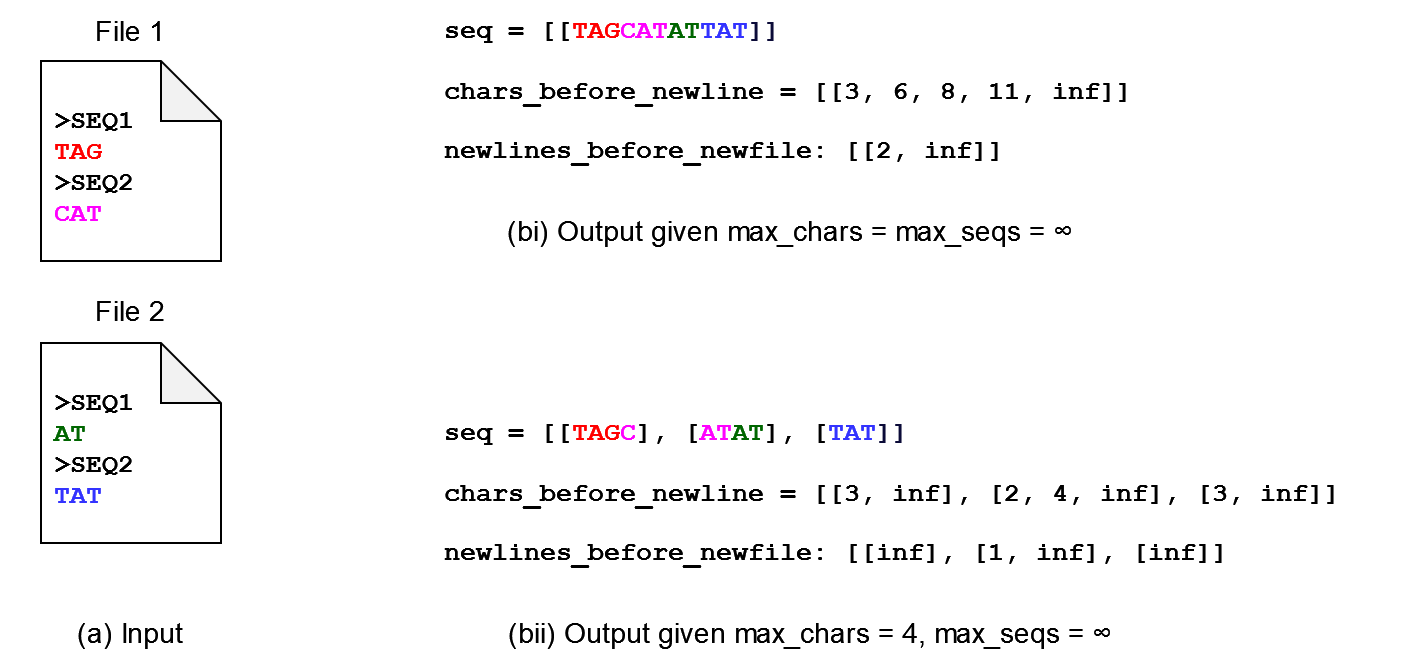
\includegraphics[width=\textwidth]{images/FastaqParser.png}
  \caption{(a) The input FASTA/FASTQ files with the sequences. (b) Outputs of the custom parser. In (bi) the entirety of the input in a single batch is read, whereas three batches are needed in (bii) since the maximum characters per batch is four. Sequences are color coded for easier interpretation.}\label{fig:FastaqParser}
\end{figure}

As a result of more logic involved with this parser, the performance is usually a bit slower than kseq++.
To test this, a FASTA file containing the human genome\footnote{\url{https://www.ncbi.nlm.nih.gov/projects/genome/guide/human/index.shtml}}\footnote{\url{https://ftp.ncbi.nlm.nih.gov/refseq/H_sapiens/annotation/GRCh38_latest/refseq_identifiers/GRCh38_latest_genomic.fna.gz}} and a FASTQ file from a study of early-life microbiota construction\footnote{\url{https://www.ebi.ac.uk/ena/browser/view/PRJEB32631}}\footnote{\url{ftp://ftp.sra.ebi.ac.uk/vol1/fastq/ERR340/004/ERR3404624/ERR3404624_1.fastq.gz}}~\cite{ecoli_genomes_3} were used.
The results and sizes of the files are shown in Table~\ref{tab:KlibVsReklib} and show that kseq++ is usually faster, especially for unzipped FASTA files.
These results were run on the Mahti supercomputer, whose specifications are discussed in Chapter~\ref{ch:Results}.
For decompression, zlib\footnote{\url{https://github.com/madler/zlib}} is used, the same as kseq++.
However, when parsing FASTQ, kseqpp\_REad is very comparable and since most of what the algorithm will be parsing are FASTQ files, as this use case deals with reads and not genomes, the performance drop is acceptable.
One disadvantage of kseqpp\_REad is that the title and quality string information are lost, so it cannot be applied to all workflows.

\begin{table}[]
\centering
\caption{Benchmarking results of kseq++ vs kseq++\_REad when parsing FASTA and FASTQ files in both zipped and unzipped formats. These values are averaged over 5 runs.}\label{tab:KlibVsReklib}
\resizebox{\textwidth}{!}{%
  \begin{tabular}{@{}lllll@{}}
  \toprule
                          & FASTA (2.2 GB)        & FASTA-zipped (928 MB) & FASTQ (3.1 GB)   & FASTQ-zipped (928 MB) \\ \midrule
  kseq++ time             & 2.2s                  & 13.5s                 & 3.7s             & 15.3s    \\
  kseq++ throughput       & 1024 MB/s             & 68 MB/s               & 838 MB/s         & 61 MB/s    \\
  kseq++\_REad time       & 4.2s                  & 15.2s                 & 4.1s             & 15.7s    \\
  kseq++\_REad throughput & 523 MB/s              & 61 MB/s               & 756 MB/s         & 59 MB/s    \\ \bottomrule
  \end{tabular}
}
\end{table}

\subsection{Preprocessing}

There are 2 steps for preprocessing the dataset.
The first is to bitpack it.
This means that the algorithm scans through the sequence produced by the previous step and converts $A$s to 0s, $C$s to 1s, $G$s to 2s and $T$s to 3s.
In binary, these can be represented with just 2-bit per character.
Thus, a u64 vector is created and the characters are packed in this vector in their original order.
This pass can be done in parallel, such that each thread processes the same amount of characters rounded to the nearest index which is a multiple of 64.
For example, given 200 characters, and 2 threads, thread 0 would process characters from 0 to 128, while thread 1 would process the rest.
In this small example, the ratio between the work done by the two threads is significant, as one thread does almost twice as much: $128 / (200 - 72) = 1.78$.
However, given that the number of characters in this case is in the order of millions or billions, one can say that each thread does the same amount of work.

During the same pass as bit-packing, another boolean vector of invalid characters is filled.
An invalid character is one which is not in the alphabet $ACGT$.
At the start, this vector is filled with 0s.
When an invalid character is seen in the sequence at an index $i$, the value of the invalid characters vector at index $i$ is set to 1.
Since this work is done in the same pass as bit-packing, it is also done in parallel, with the bitvector reserved beforehand.
Rather than a vector of booleans, in the implementation a vector of characters is used, as it was found to be faster.
When an invalid character is found, it is represented as if it were an A when it is bit packed, that is, as $00$.

The last preprocessing step is building the positions vector.
As discussed before, if a sequence has $C$ characters, then it has $C - k + 1$ $k$-mers.
The positions are thus u64s which represent the indexes in this sequence where a $k$-mer starts, and the next k characters, that index included, will be considered as a $k$-mer.
To do this position building, the chars\_before\_newline created in the parsing phase are used.
The positions can be generated with a single pass over this vector.
Figure~\ref{fig:Preprocessing1} shows an example of the preprocessing outputs discussed in this subsection.

\begin{figure}[t]
  \centering
  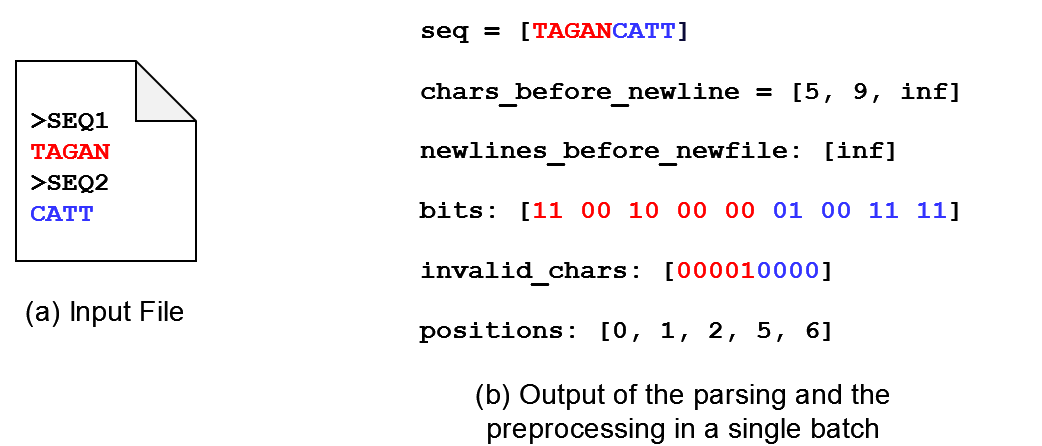
\includegraphics[width=0.8\textwidth]{images/Preprocessing1.png}
  \caption{An example of parsing and preprocessing in a single batch with the maximum characters per batch being $\infty$} \label{fig:Preprocessing1}
\end{figure}

The algorithm uses batching, so that each batch can only have a maximum number of characters and a maximum number of new sequences, whichever is reached first.
Since batching is being used, trouble would ensue if batching breaks a sequence in half, since characters may be shared between $k$-mers.
Hence the final $k-1$ characters must be copied from the previous batch to the start of the new batch in order not to miss any $k$-mers.
The amount may be less than this, as there is only a need for copying if the batching breaks the $k$-mers.
Figure~\ref{fig:Preprocessing2} shows an example where one needs to copy, and a case where copying is unnecessary.
There are also middle cases where one may need to copy some characters but less than $k-1$ characters.
This happens when the batching cuts off a sequence at its beginning, that is, before k characters have been parsed from it.
Copying is done in the parsing step, the first step discussed, so the rest of the components are oblivious to this step.

\begin{figure}[t]
  \centering
  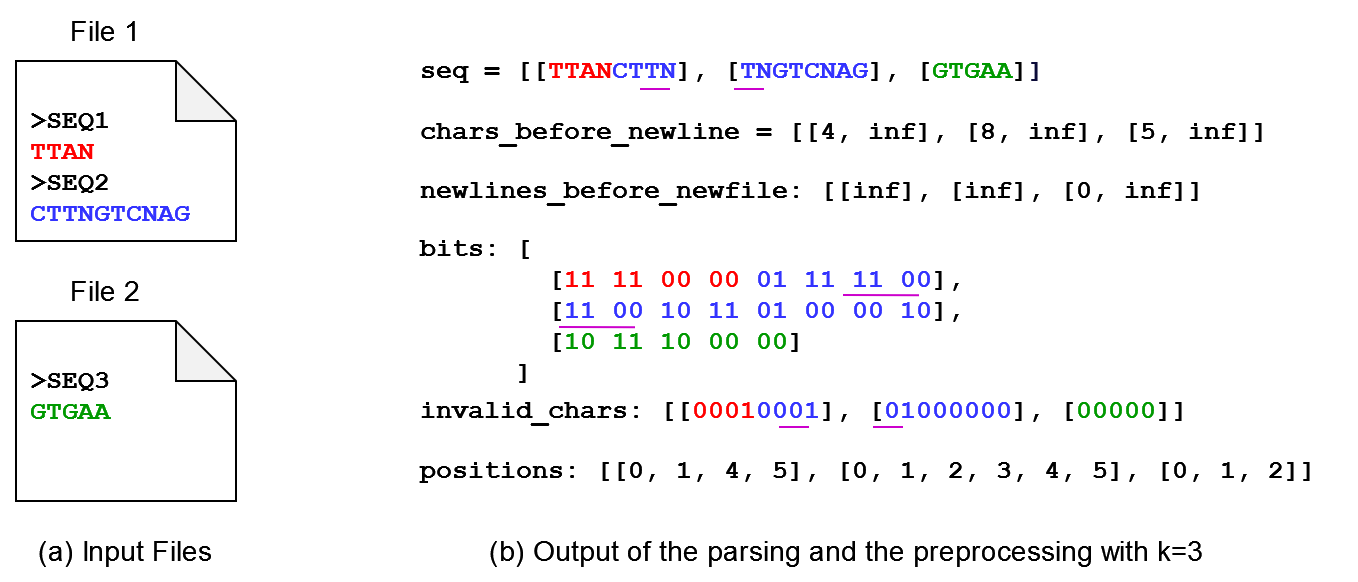
\includegraphics[width=\textwidth]{images/Preprocessing2.png}
  \caption{A second example of preprocessing, with the maximum characters per batch being 8. Notice how the string gets broken between the first and second batch, but not between the second and third. Overlapping areas have been marked with purple lines.}\label{fig:Preprocessing2}
\end{figure}

\subsection{Searching}

The index searching algorithm was discussed in Section~\ref{sec:SBWTQuerying}.
The only difference now is that the processing is done on the GPU.
Remember that the SBWT, the Poppys and the key-$k$-mer marks are already copied to the GPU.
Now the bit-packed sequence and the positions also need to be copied there.
Thus, each thread on the GPU handles a single position, since there is no relation between one $k$-mer search and the next.
As an optimisation, to save memory, and perform less memory accesses, one can overwrite the u64s of the positions with the u64s of the search result.
After this, the results can be copied back to memory and written to disk.
This GPU search function was created previously~\cite{Harri} but is now refactored and used in the new solution.
One change that this thesis has made to the previous implementation is to make it possible to query for $k > 32$ by always querying global GPU memory for the next two bits, rather than first storing the entire $k$-mer into a u64 and then querying that.
Although the performance difference between the previous and new kernel was not measured in isolation, this change was not shown to impact the overall performance of the algorithm from start to finish, since the kernel is only a small part of the bigger picture.

One more optimisation to searching which was used in previous works is presearching \cite{Presearch, SBWT, Harri}.
This is done right after loading the SBWT to the GPU, however, it was chosen to discuss it now in order not to confuse the reader with too much disjoint information at the beginning.
The notion behind presearching is that one can search for the first part of the $k$-mers beforehand, store these in memory, so then rather than recomputing these, they can be loaded from memory and continue the search continues from there.
To do this presearching, the left and right pointers are moved forward by a certain amount $k_p$ for every permutation of a $k_p$-mer.
Thus, given for example $k_p=2$, the combinations are: $AA, AC, AG, AT, CA, CC, \ldots, TG, TT$.
Represented as binary, they become: $0000, 0001, 0010, 0011, 0100, 0101, \ldots, 1110, 1111$.
The decimal representation is then: $0, 1, 2, 3, 4, \ldots, 14, 15$.
Thus note that these can be used as the indexes to both store and later retrieve the presearched left and right pointers for $k_p$.

In the example, 16 memory spaces are needed.
More generally, $4^{k_p}$ are needed for each of the left and right pointers, where each memory space contains a u64.
Thus, the final formula for the total number of bits to store the presearch results is \[4^{k_p} \times 64 \times 2 \quad \mathit{bits}.\]
Ideally, one would presearch with $k_p = k$, however, the memory requirements for this would be massive, as the formula is exponential on $k_p$.
If $k_p=k=31$, this would require $4^{31} * 64 * 2 / 8 / 1024 ^ 3 \approx 9$ billion GB.
As a result, similar to the previous GPU method~\cite{Harri}, $k_p=12$ is used.
With this, 250MB of data are needed in total for the presearch data.
Algorithm~\ref{alg:SearchWithPresearch} shows the final search algorithm.

\begin{algorithm}
	\KwIn{\newline
    A sequence $S = c_1, c_2, \ldots, c_k$ \newline
    Bitvectors $b_A, b_C, b_G, b_T$
    c-map $C$
    Presearch size $k_p$
    Presearch maps $presearch_{\mathit{left}}$ and $presearch_{right}$
	}
  $\mathit{left}$ = $presearch_{\mathit{left}}[c_1, \ldots, c_{k_p}]$

  $\mathit{right}$ = $\mathit{presearch}_{right}[c_1, \ldots, c_{k_p}]$

  \ForEach{c \textbf{in} S[($c_{k_p} + 1$) \ldots k]}{
    $\mathit{left}$ = $C[c]$ + rank ($b_c$, $left$)

    $\mathit{right}$ = $C[c]$ + rank ($b_c$, $right + 1$) \-- 1

    \If{$\mathit{left}$ > $\mathit{right}$} {\
      \textbf{return} not found
    }
  }

  \textbf{return} $left$

  \caption{Index Search function with presearch.}\label{alg:SearchWithPresearch}
\end{algorithm}

\subsection{Results Printing}

For results printing, there are three output formats, but programmatically they follow the same interface.
This means that in general, they all print to a memory buffer first and then these buffers are printed to disk.
Printing to buffers is done in parallel, meaning that each thread has an equal amount of indexes to print and each thread prints to its own equally sized buffer, and then the buffers are printed to disk sequentially.
The reason it was opted to parallelise this pass, rather than simply printing to disk, is because of the conversions which need to be done, from the binary representation in memory, to the representation on disk.
For this step, the search results are used, the chars\_before\_newline to know where to split each sequence, the seqs\_before\_newfile to know when the algorithm needs to open the next file, and the invalid characters list to differentiate these from the characters which were not found.
The feature to differentiate invalid characters from the not-founds is not found in Themisto or its precursors, and is hence another new contribution.

Next, each output format is discussed.
Figure~\ref{fig:IndexResultsPrinting} serves as a good visualisation of how the characters are written to disk.
It is important to note that the only implementation difference between these formats is how they print each value.
The available values which they can print are the following: a found index, a not-found index, an invalid character, or a newline.
The first to consider is the ASCII format, where the indexes are printed as a space-separated list of values.
The values for the indexes are simply u64s, so they can be printed as their ASCII counterparts.
The not-found values are represented as $-1$, invalid characters as $-2$, and newline values as the expected line feed character \textit{\textbackslash n}.
This format was the one that saw the largest benefit from parallelisation, as the operation to convert from binary to ASCII, especially for larger numbers, takes significant CPU time, due to the need of performing many division and modulus operations which are computationally expensive.
In order to convert from binary to ASCII, the algorithm created by James Anhalt\footnote{\url{https://github.com/jeaiii/itoa}} is used.
This was benchmarked on a dummy dataset internally against the \textit{to\_string} algorithm from the GCC C++ standard library and against the \textit{format\_decimal} algorithm by \textit{fmt}\footnote{\url{https://github.com/fmtlib/fmt}} library and it was found that the algorithm by Anhalt was significantly faster than these alternatives.
It is also the fastest algorithm in other benchmarks\footnote{\url{https://jeaiii.github.io/itoa/}}.
No detail will be given as to how the u64 to ASCII algorithm works and what differentiates it from other algorithms, as this problem is a deep rabbit hole and could make for its own thesis.

\begin{figure}[t]
  \centering
  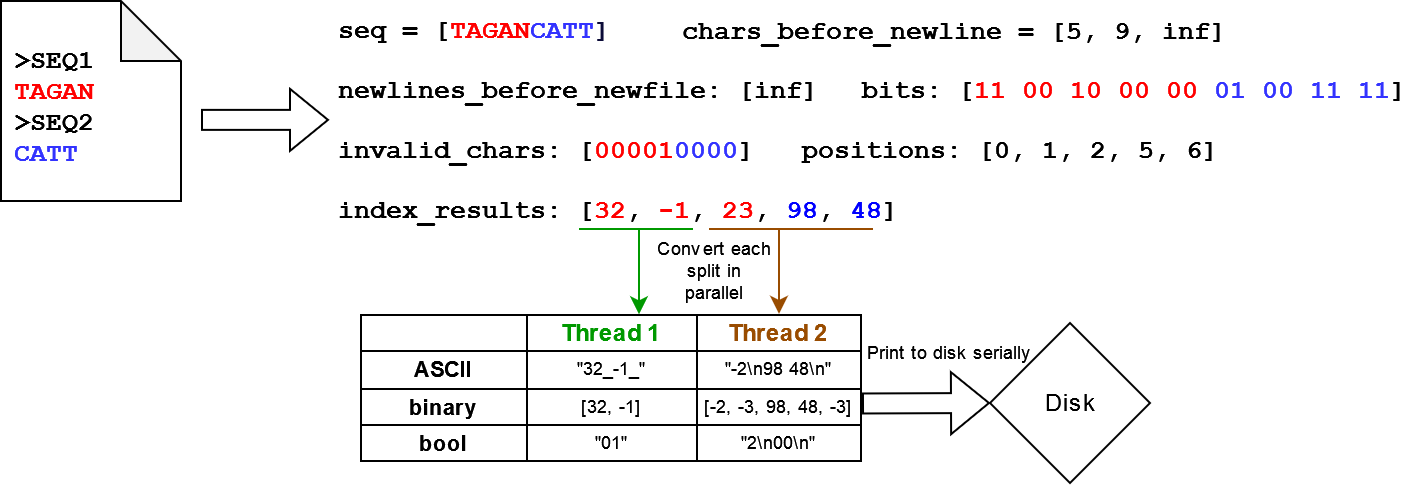
\includegraphics[width=\textwidth]{images/IndexResultsPrinting.png}
  \caption{The results printing pipeline from FASTA/FASTQ files to printing to disk in a single batch. The parallelisation of this is also visualised. For the ASCII and bool formats, these use usual 8-bit ASCII characters for their representation, whereas for the binary format uses a contiguous array of u64s.}\label{fig:IndexResultsPrinting}
\end{figure}

The second format is the binary format.
In this format, each element that is printed takes 8 bytes, as everything is printed as a u64.
Results are printed as they are.
Meanwhile, not-found values are printed as the maximum u64 value, that is, $2^{64}$, invalid values are printed as $2^{64} - 1$, and newlines are printed as the $2^{64} - 2$.
In C++, unsigned integers loop back when they overflow, so that one can say that the values for not-founds, invalids and newlines are $-1$, $-2$, and $-3$ respectively.
This method would be faster and with less memory requirements than the ASCII format if most of the indexes contain more than 8 bytes.
The ASCII format requires at most 20 bits for each character, since the maximum value of u64 is 20 characters long, plus another character for the whitespace character which separates the values.
However, as will be seen in Chapter~\ref{ch:Results}, while not drastically slower than the ASCII format, this method ends up taking a lot more space, since the indexes are usually not too large.

The last format is dubbed the boolean format.
In this format, the sequences are separated with newlines, as in the ASCII format.
However, for the values, a single byte is used.
For the found values, the ASCII character for 0 is printed, then the not-founds are represented with a 1 and the invalids are represented with a 2.
This makes it the smallest format and also also the fastest to print, at the cost of losing the index information, that is, where the $k$-mer is found within the SBWT.
As a result, it is not suitable for the second phase, since the indexes are needed.
However, it is the best format for users who simply want to know if the $k$-mers of their sample exist within the SBWT or not.

\section{Phase 2:  Color Search}

Now the color searching phase will be described.
A small summary is the following: (a) Load the color data structure from disk into the GPU, (b) parse the indexes output of phase 1 from disk and put them in the GPU, (c) search for the color set associated with each index within the GPU, (d) combine all the colors of a sequence together in the GPU, (e) copy the results back from GPU into main memory and write the color sets for each sequence to disk.
Each of these steps, how they are parallelised, and what data structures they produce will be elaborated on in the next section.
Similarly to the index search, the data structures introduced in this section are summarised and explained in a different manner to aid understanding, in Appendix~\ref{app:ColorSearchDataStructures}.

\subsection{Preliminaries and Definitions}

Before discussing the implementations, some mechanisms of how work is done in the GPU need to be introduced.
A unit of work on the GPU is done with a \textit{warp} (or \textit{wave} in AMD terminology).
Each warp in an NVIDIA GPU consists of 32 threads, and 64 in an AMD GPU.
This means that threads within a warp execute at the exact same time under normal conditions.
Threads in a warp can also communicate with one another by sharing the contents of their variables, using what are known as shuffle operations\footnote{\url{https://people.maths.ox.ac.uk/gilesm/cuda/lecs/lec4.pdf}}\footnote{\url{https://docs.nvidia.com/cuda/cuda-c-programming-guide/index.html#warp-shuffle-functions}}\footnote{\url{https://developer.nvidia.com/blog/using-cuda-warp-level-primitives/}}.
For example, if each thread has a variable $X$, this can be broadcasted to all the threads in the same warp.
One common use case of this feature is to get the sum of the variable across the warp.
Another approach is shared memory\footnote{\url{https://docs.nvidia.com/cuda/cuda-c-programming-guide/index.html#shared-memory-variable-declarations}}, which works on the block level.
However, neither shared memory nor blocks will be discussed since they are irrelevant to the rest of the thesis.

A point to remember from Section \ref{sec:Pseudoalignment} is that all $k$-mers in the SBWT are colored, except for dummy $k$-mers.
This means that if a $k$-mer is found in the SBWT, it is colored, and if not, then it is blank.
In this thesis, a colored sequence means refers to sequences that have at least one found $k$-mer, otherwise the sequence will be a \textit{blank sequence}.

\subsection{Loading the Colors}

Now starts the implementation part of this section, with the description of how the colors are loaded.
This data structure is created by Themisto, and needs to be loaded from disk.
The data structure itself is described in Section~\ref{sec:Pseudoalignment}, and all that is added is that the Poppy data structures need to be built for the $\mathit{is\_key\_k\_mer}$ and $\mathit{is\_dense\_marks}$.
This data structure also contains some additional variables such as the number of colors $\mathit{num\_colors}$.
The process is done entirely serially as the items are loaded from the file and the Poppy of the bit-vectors is created serially as well.
These components are then all loaded into GPU memory and kept there until the end.

\subsection{Loading the Indexes}\label{subs:IndexesLoading}

Now the indexes are loaded from disk as they were printed in phase 1.
For this subsection, Figure~\ref{fig:IndexesLoading} shows the final product.
For each sequence the count is taken of how many indexes were found, not found, or are invalid.
Similarly to the first phase, a vector is also created, called the $\mathit{seqs\_before\_newfile}$, which stores a cumulative sum that indicates at which point the algorithm needs to stop considering sequences to be from one file and start considering them as originating from the next file.
A new count is started at the very beginning of a batch or whenever a newline symbol is seen, these symbols being the line feed character '\textbackslash n' for ASCII and a -3 for the binary format.
Again, the boolean format is not suitable for pseudoalignment and cannot be used for phase 2 since this method does not have the indexes.
Similar to reading in phase 1, batching is used with a set maximum number of characters and maximum number of sequences per batch.

For parsing, no special techniques are used.
Characters are read one by one, and for the ASCII format, the na\"ive method of reading one digit and adding it to the previous value multiplied by 10 is used.
This is faster than the C++ standard library, as the standard library implementations usually have some form of error checking involved.
For the binary format, the algorithm simply reads 64 bits at a time.

\begin{figure}[t]
  \centering
  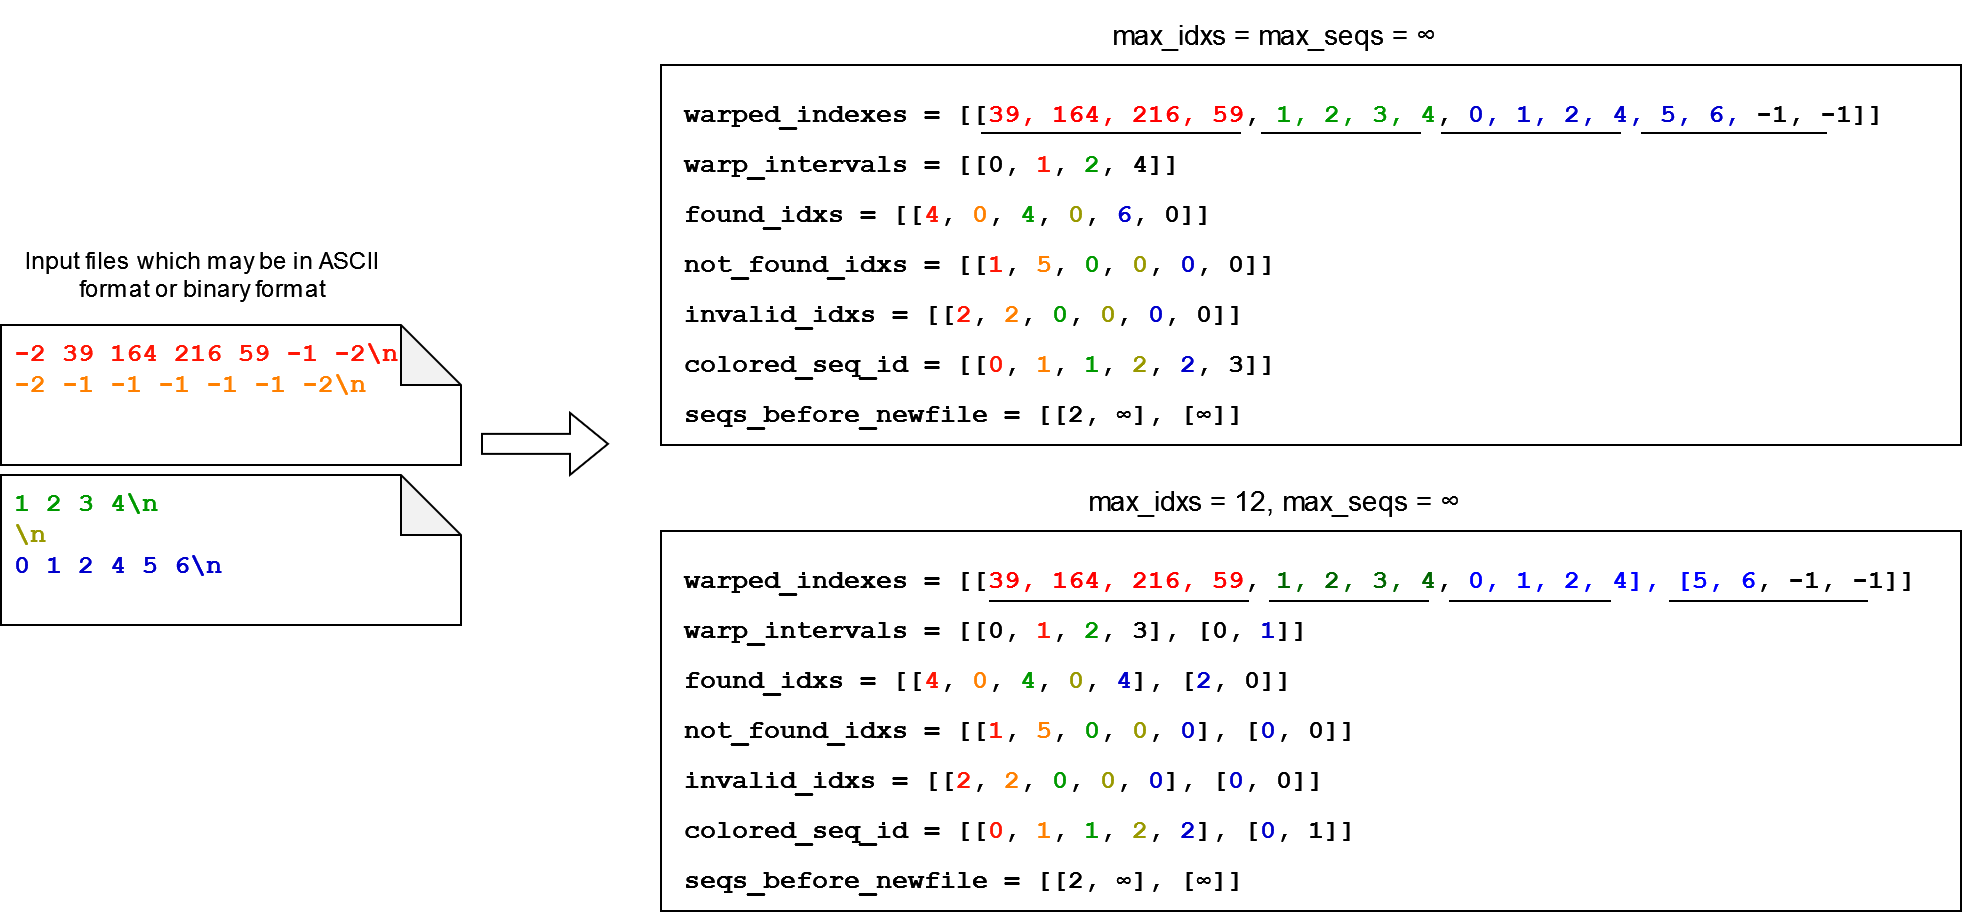
\includegraphics[width=\textwidth]{images/IndexesLoading.png}
  \caption{Example of loading from an ASCII or binary index files and populating the necessary data structures with two different configurations, one where the maximum characters per batch is infinite and one where it is limited to 12, such that the last sequence is broken in two. Note that the last values of the $\mathit{found\_idx}$, $\mathit{not\_found\_idx}$, $\mathit{invalid\_idx}$ and, $\mathit{colored\_seq\_id}$ are because the algorithm needs to consider the next sequence to come.}\label{fig:IndexesLoading}
\end{figure}

Indexes that are not found or invalid are not stored.
This makes the algorithm a lot more efficient, both in terms of time and memory.
The respective counters for the sequence that these indexes belong to are increased, but they are not stored as part of the index list.
Thus, blank sequences effectively take no space, besides the small variables for their counters.
Meanwhile, the indexes of colored sequences are stored contiguously, but between one sequence and the next, padding is used up to the next multiple of the warp size.
This technique and the reasoning for it will be made clearer in Subsection~\ref{subs:ColorSearch}.

Since a sequence may be larger than the warp size, these $\mathit{warped\_indexes}$, as they are called, are then separated via another list called the $\mathit{warp\_intervals}$.
The first entry of this list is always 0, and another entry is added whenever a new sequence causes more $\mathit{warped\_indexes}$ to be added which belong to a new sequence.
Whenever that happens, the new entry which is added will be the cumulative sum of how many warps the algorithm has until the end of that sequence.

Besides the aforementioned variables, another list exists and is called the $\mathit{colored\_seq\_id}$.
This stores an unsigned integer for every sequence, and it indicates which number colored sequence this sequence is.
If a sequence is blank, a $\mathit{colored\_seq\_id}$ is still stored for it, and for convenience, the previous in the list is copied for it, but it might as well be padding as it is later ignored.
This list is then is used in Subsection~\ref{subs:ColorsPrinting}.

\subsection{Searching}\label{subs:ColorSearch}

The next part is the color searching, which is entirely done on the GPU but is split into two kernel calls: Searching and Post Processing.
First, the indexes are copied to the GPU and memory is reserved for the color results.
Note that since blank sequences do not produce any indexes, they also do not use any computations on the GPU later on, thus the algorithm runtime depends on the number of warps spanned by the colored sequences.
Next, the values reserved for the color results are set to 0 using \textit{memset}.
Each thread handles a single index and searches for its color set type, which is sparse or dense, its start index, and its end index, using the same method as Algorithm~\ref{alg:ColorSearch}.
If a thread has a padding index, then it exits immediately.
To do this, a separate GPU functions gets booleans from bitvectors and another extracts a normal u64 from the compact vectors.
The result of this step are the indexes where the color sets start and end within their respective dense or sparse arrays.

The next step of the kernel is to extract and combine the color sets.
First, a small optimisation is performed, which is to get the minimum and maximum color id which exists within the color set of each thread.
To get the minimum present color of a dense color set, the algorithm iterates through the bitvector from the starting point of the color set until the first set bit is found.
Then, to get its maximum, it can simply negate the end index of this color set with the starting index, both of which were found before.
On the other hand, to get these values for sparse colors, one needs to access the sparse color set array and obtain the ones at the start and end indexes to get the minimum and maximum present color id respectively.
Next, an XOR shuffle is performed to broadcast these two values to the other threads inside the warp, so that each thread knows the minimum and maximum color if of all threads within the warp.
To broadcast a value using shuffle, the algorithm needs to perform $log_2(warp\_size)$ steps, as is visualised in Figure~\ref{fig:ShuffleXor}.
Two shuffles need to be performed: one for the minimum and another to broadcast the maximum.
Due to the padding technique when reading the indexes, all threads in each individual warp only contain indexes belonging to a single unique sequence, that is, a warp will not mix colors of different sequences together.

\begin{figure}[t]
  \centering
  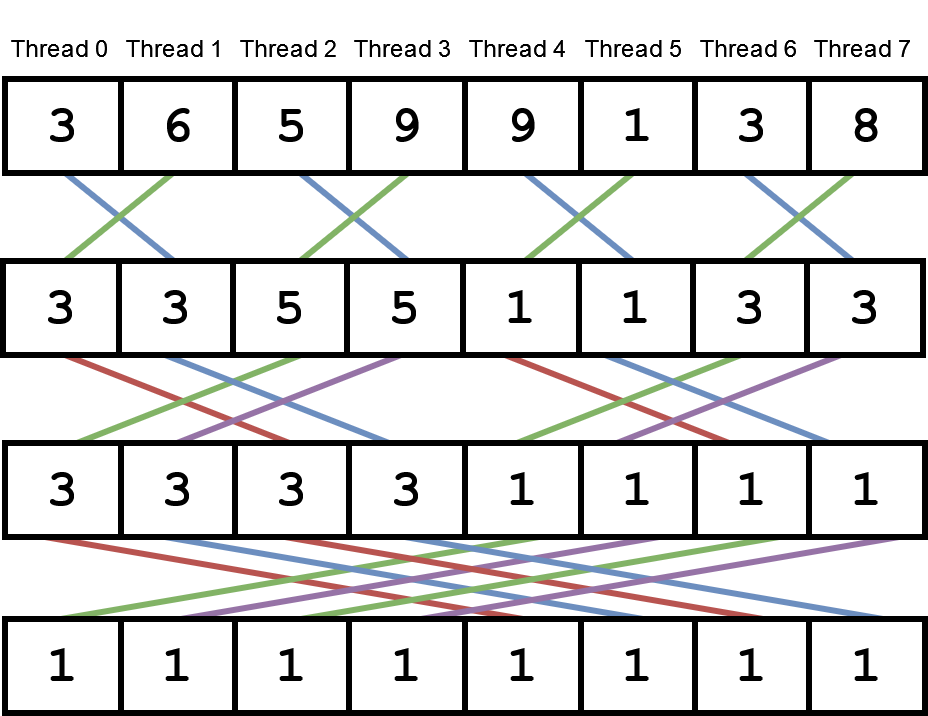
\includegraphics[width=0.7\textwidth]{images/ShuffleXor.png}
  \caption{An example of how data is shared between threads at each step of an XOR shuffle operation to find the min value of the warp. The warp size for this visualisation is 8, hence there are $log_2(8) = 3$ shuffle operations.}\label{fig:ShuffleXor}
\end{figure}

The next step is to iterate through all the colors in the color sets from the minimum and maximum of the warp, and set a boolean value to whether the color exists in the color set of that thread or not.
To get the color presence in the dense array, one can simply do a boolean access in the bitvector at the index of the color.
When it comes to the sparse array, one then needs to go through the array and check if the current color id matches the value in the array.
Luckily the sparse arrays are sorted so the algorithm can do this check in a single step, without going through the whole array for every query, thus going through the whole array only once, as the color presence of every color is checked.

After the color presence of a color is obtained, $\mathit{ballot()}$ is called, where an unsigned integer is created which has as many bits as the warp size, and each thread in the warp sets its respective bit in this integer to 1 if the color is present, and 0 otherwise.
The result of this ballot is broadcasted to all threads in the warp, but it is thread 0 that performs a popcount on this result and stores the color count to device memory.
Notice that this result is at most 32 in the case of NVIDIA devices, and 64 in the case of AMD devices.
This means that a 32-bit integer representation is used for the NVIDIA case, and a 64-bit integer is used for AMD devices.
Furthermore, it also means that the popcount of each of these color counts can be stored in an 8-bit unsigned integer, which is why a list of u8s is used to store these intermediate results, in order to save memory space and thus be able to process more indexes per batch.
The $\mathit{ballot()}$ function is visualised in Figure~\ref{fig:Ballot}, whereas the pseudo code until this point of the color search is found in Algorithm~\ref{alg:GpuColorSearch}.

\begin{figure}[t]
  \centering
  
\includegraphics[width=0.7\textwidth]{images/Ballot.png}
  \caption{An example of a ballot operation for a warp of size 8. The ballot operation is called only once in each of the threads, whereas the popcount function on the result of this operation needs to be called by thread 0 only, since this is the one which will be storing the result in this case.}\label{fig:Ballot}
\end{figure}

\begin{algorithm}
	\KwIn{ \\

    $\mathit{warped\_indexes}$

    $\mathit{warp\_size}$

    $\mathit{num\_colors}$

    $\mathit{dense\_arrays}$

    $\mathit{sparse\_arrays}$
	}

  $\mathit{thread\_idx}$ = GPU thread id

  $i$ = $\mathit{warped\_indexes[thread\_idx]}$

  Get $\mathit{start}$, $\mathit{end}$ and $\mathit{is\_dense}$ using $i$ as an input to Algorithm~\ref{alg:ColorSearch}.

  \If{$\mathit{is\_dense}$} {\newline

    $\mathit{min\_id}$ = Traverse $\mathit{dense\_arrays}$ from $\mathit{start}$ to get first set bit

    $\mathit{min\_non\_zero\_color}$ = $\mathit{start}$ - $\mathit{min\_id}$

    $\mathit{max\_non\_zero\_color}$ = $\mathit{end}$ - $\mathit{start}$

  }\Else{ \\

    $\mathit{min\_non\_zero\_color}$ = $\mathit{sparse\_arrays[start]}$

    $\mathit{max\_non\_zero\_color}$ = $\mathit{sparse\_arrays[end - 1]}$
  }

  $\mathit{min\_non\_zero\_color}$ = xor\_shfl($\mathit{min\_non\_zero\_color}$)

  $\mathit{max\_non\_zero\_color}$ = xor\_shfl($\mathit{max\_non\_zero\_color}$)

  $\mathit{array\_idx}$ = $\mathit{start}$

  \ForEach{$\mathit{color\_id}$ \textbf{in} [$\mathit{min\_non\_zero\_color}$ \ldots $\mathit{max\_non\_zero\_color}$]}{

    \If{$\mathit{is\_dense}$} {\newline

      $\mathit{color\_present}$ = ($\mathit{dense\_arrays[array\_idx]}$ = 1)

      ++$\mathit{array\_idx}$

    }\Else{\newline

      $\mathit{color\_present}$ = ($\mathit{sparse\_arrays[array\_idx]}$ = $\mathit{color\_id}$)

      \If{$\mathit{color\_present}$} {\newline

        ++$\mathit{array\_idx}$
      }
    }

    $b$ = ballot($\mathit{color\_present}$)

    \If{$\mathit{thread\_idx}$ \% $\mathit{warp\_size}$ = 0} {\newline
      $\mathit{results}$[$\mathit{num\_colors}$ * $\mathit{thread\_idx}$ / $\mathit{warp\_size}$ + $\mathit{color\_idx}$] = pop\_count($b$)
    }

  }

  \caption{GPU Color Search}\label{alg:GpuColorSearch}
\end{algorithm}

The result of this step is a color count for each color for each warp, where many warps may belong to the same sequence.
Thus, the last step is to postprocess the results by combining the results of the same sequence into a single list.
First, memory is reserved for these u64 results and the warp intervals created in Subsection~\ref{subs:IndexesLoading}, the latter of which can now be copied to the GPU.
Both of these two arrays use the same memory space previously used by the indexes, to maximise memory usage.
Now, one thread is created for every color in every sequence.
Each thread gets a cumulative sum of a single color in the whole sequence and then stores this sum in the new u64s.
These final results can then be copied to CPU memory, as they are now ready for printing.
A visualisation for the post processing step is in Figure~\ref{fig:PostProcessing}.
The disadvantage of this postprocessing method is that if the number of indexes in the colored sequences varies by a lot, then the sequences would produce a disproportionate number of color sets, meaning that some threads would need to do more work.
Luckily, the ballot step of the first phase reduces the work done in this step and the memory required by a factor of 32 on NVIDIA devices and a factor of 64 on AMD devices.
These two factors, that is, both the work done and memory used, is also the reason why it was opted to only put and process colored sequences in the GPU.
Also notice that some threads will only need to only expand the value of the color id from u8 to u64 and store it into the new results, without doing any additions.
Moreover, a flaw of this design is that, given sparse color sets, that is, most colors result in a count of zero, then this design ends up wasting a lot of space, as these zero counts still need to be allocated and also copied back to CPU memory.

\begin{figure}[t]
  \centering
  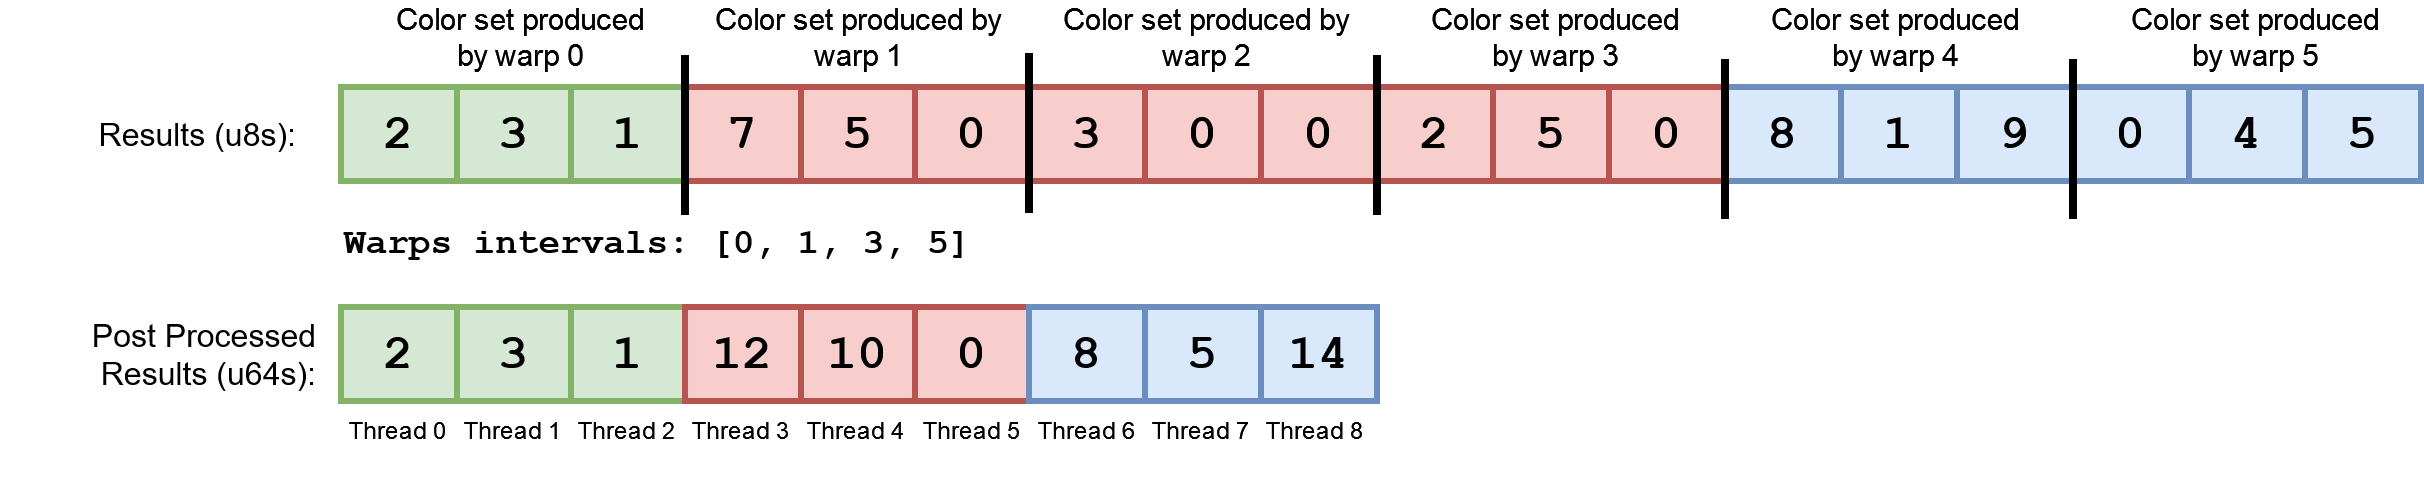
\includegraphics[width=\textwidth]{images/PostProcessing.png}
  \caption{A visualisation of the post processing done on the colors. Each thread handles a single color from each sequence. As a result, some threads may end up doing more work than others if a different number of $k$-mers are found from each sequence. In this case, the middle sequence had more $k$-mers found, which meant that it produced more color sets: 3 warps worth of color sets. Hence, the post processing step does 3 sums for this sequence.}\label{fig:PostProcessing}
\end{figure}

\subsection{Results Printing}\label{subs:ColorsPrinting}

The final step of this last phase is to print the results.
In order to print, besides the colors themselves, the counts for the found, not-found and invalid indexes are provided, alongside the $\mathit{coloured\_seq\_id}$ and the $\mathit{seqs\_before\_newfile}$.
Similarly to the results printing in the first phase, the results are first printed to buffers in parallel and are then printed to disk serially.
For this phase, there are also three output formats: ASCII, binary, and CSV.
In the ASCII format, the colors are printed as space-separated values, where the color id is printed if it appears in the sequence, and each sequence is put on its own line.
Similarly to the previous phase, the boolean format prints each color as a u64 sequentially, where the maximum u64 is used to represent a new line.
These two formats could be seen as the sparse representation outputs, and the CSV is the dense output.
The CSV format prints a comma separated 1 or 0 for each color, where 1 means that the color is present in that sequence and 0 means it is not.
Figure~\ref{fig:ColorsPrinting} shows an example of these three results formats.

When printing to buffers in parallel, each thread handles an equal number of sequences, whether colored or not.
This may lead to some threads doing more work, as colored sequences take much longer to process for the ASCII and binary formats, especially when the color set size is big.
Reads, however, are usually distributed randomly, so the threads should statistically do the same amount of work
Before printing, thresholding is also done in this part.
The contribution of this thesis to this space is the differentiation between thresholding invalid $k$-mers as well as $k$-mers which were not found, the latter of which was included in Themisto.
So the user can choose to ignore one of them, both, or none at all.
Another advantage over Themisto is that the results are always output in ascending order, whereas Themisto may shuffle the results within a single sequence.
Lastly, since a sequence may be split into two batches, the colors and other sequence properties of the last sequence of a batch are copied over to the first sequence of the next batch in order not to lose any information.

\begin{figure}[t]
  \centering
  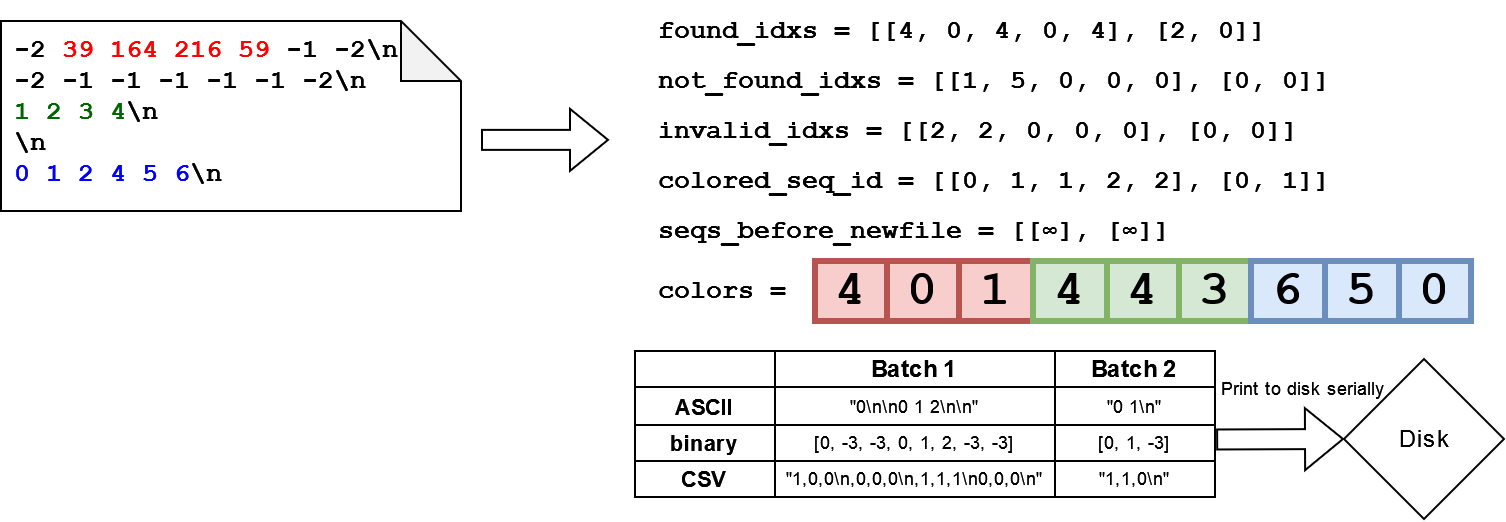
\includegraphics[width=\textwidth]{images/ColorsPrinting.png}
  \caption{A visualisation of the printing of the colors in all three formats. Here, $\tau=0.7$ is used, ignoring the kmers which are not found or invalid.}\label{fig:ColorsPrinting}
\end{figure}

\section{Other Optimisations and Parallelism}

In this section general optimisations used throughout the algorithm will be described.
These were not discussed during the general discussion of the two phases as they were not necessary to understand those topics, and they would have added a lot of complexity to an already complex topic.

\subsection{Curiously Recurring Template Pattern (CRTP)}

The first and simplest optimisation is the Curiously Recurring Template pattern which is popular for C++ development.
For those unfamiliar with C++, when a child class inherits a parent class and polymorphism takes place, a virtual table is created, which indicates the correct function to call to the program.
Thus, when a call to an inherited function is done, another call to the virtual table must be done, which is usually expensive as it requires another memory access.
CRTP allows programmers to do inheritance without the need for virtual tables, with the penalty being the use of templates, which make the code slightly less maintainable.
This optimisation was especially beneficial for the results printing, as some of the methods there are called billions of times, and traditional inheritance is still used in a lot of places where methods are not called as often.

\subsection{Multithreaded Pipeline}

In the two phases, there are some components that are dependent on one another, and others that are not.
Furthermore, since it is a pipeline, an earlier component can start processing the next batch while the later component is processing an earlier batch.
This is done by inheriting all producer components from a parent component called the \textit{SharedBatchesProducer}.
By using semaphores, it is ensured that all components can run in parallel, while still being able to share the memory of the buffers that the producers and consumers share safely.

\subsection{Pinned Memory}

For variables that need to be copied to and from the GPU, it is possible to use pinned memory on the main memory in order to speed up memory transfers.
To do this, all the programmer needs to do is to reserve the memory space beforehand using \textit{cudaMallocHost}\footnote{\url{https://docs.nvidia.com/cuda/cuda-runtime-api/group__CUDART__MEMORY.html}} or \textit{hipHostMalloc}\footnote{\url{https://rocm-developer-tools.github.io/HIP/group__Memory.html}} if using HIP.
Pinned memory can be copied to the GPU directly, whereas more care needs to be taken by pageable memory as this could be moved while copying is taking place, whereas pinned memory is guaranteed to remain in the same location within memory until it is freed\footnote{\url{https://developer.nvidia.com/blog/how-optimize-data-transfers-cuda-cc/}}.
This feature sped up transfers to and from GPU by almost twice, which is a significant difference for this use case as there are a lot of large transfers.
The drawback of reserving most of the memory beforehand is that large amounts of contiguous blocks need to be reserved at once.
This can be difficult to manage for the operating system, and in fact often contributes to a significant overhead at the start of the algorithm
Luckily this overhead is constant, so as the datasets get larger, this overhead becomes less and less significant, and for smaller datasets, a smaller memory can be reserved for the algorithm, which is a setting that can be altered by the user.
That said, for other variables which do not need to be communicated to or from the GPU, normal paged memory is used.

\subsection{Streams}

Often, larger datasets will be split into multiple files.
The code takes advantage of this by providing an algorithm that can take advantage of this, by being able to process multiple files at once.
This means that the pipeline is duplicated and the number of files can be split between each stream.
The term \textit{stream} is used to indicate each pipeline.
This means that, for example, given seven files and three streams, then stream 0 would handle three files, and streams 1 and 2 would handle two files each.
The two streams can then share the same SBWT or colors data structure in phases 1 and 2 respectively.

The benefit of using streams is that reading from disk and outputting to disk can also be done in parallel.
This is especially useful when using a multi-disk setup, or if the device in use can support this feature.
However, even if not using any of the above two hardware devices, two more advantages are universally applicable.
The first and more obvious is that by using streams, the CPU and disk can be kept more busy.
The second is the use of GPU streams.

Using a single stream with GPUs, the process is: (a) copy some data to the GPU, (b) do some processing, and (c) copy the data back to main memory.
By using multiple streams, each stream still does the same three steps, however, if multiple streams are used, the GPU can interleave the memory transfer of one stream with the processing of another\footnote{\url{https://developer.download.nvidia.com/CUDA/training/StreamsAndConcurrencyWebinar.pdf}}.
Memory transfers from GPU can also be interleaved with memory transfers to GPU on some devices.
Figure~\ref{fig:Streams} shows this visually.
The number of streams is configurable by the user, but is capped based on the number of files, so that the number of streams is always smaller or equal to the number of files that need to be processed.

\begin{figure}[t]
  \centering
  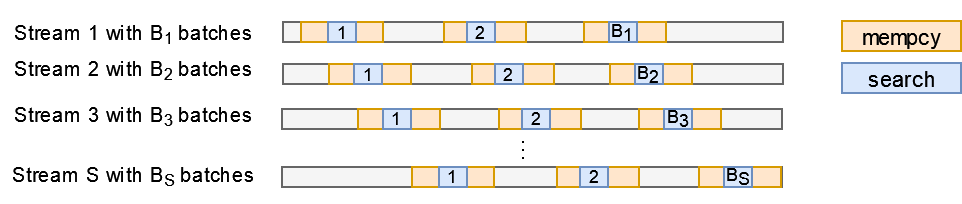
\includegraphics[width=0.8\textwidth]{images/Streams.png}
  \caption{A visualisation of using streams and their benefit on GPU processing, where memory transfers are interleaved with processing. The batch number is also displayed.}\label{fig:Streams}
\end{figure}

\subsubsection{Load Balancing}

An additional optimisation for streams is to load balance the streams.
Notice that if some files are large while others are very small, then different streams might have very different workloads.
Thus, the algorithm considers load to be based on file size.
As such, before assigning files to streams, they are analysed for their size and then a greedy algorithm called the Longest Processing Time first (LPT)~\cite{LPT1, LPT2}.
Here, an array is created for each stream, the file sizes are sorted such that the largest file is always chosen first and this file is then assigned to the array with the smallest load.
LPT is proven to be bound to give a result that is $\frac{4}{3}$ from the optimal~\cite{LPT2}.
This load balancing is done in both phases.

\subsection{Memory Reservations}

When it comes to memory reservations, all the memory allowed by the user through user input is reserved by the algorithm.
This first checks how much memory each component needs per character or per index, in phases 1 and 2 respectively, and then reserves memory accordingly, such that the batches are as big as possible without overflowing GPU or main memory.
When the algorithm has multiple streams, this memory reserved is divided by the number of streams, such that each stream gets an equal amount of memory, and thus the batch sizes are equal.
Figures~\ref{fig:IndexBatches} and~\ref{fig:ColorBatches} in Appendix~\ref{app:Batches} shows all the dependent components and the memory needed by each component.


\chapter{Results}\label{ch:Results}

The dataset consists of two parts, the indexed genomes from which the Colored De Bruijn Graph is generated, and the reads which will be pseudoaligned against this index.
Firstly, the colored DBG was built using Themisto with a dataset consisting of three collections of genomes~\cite{ecoli_genomes_1, ecoli_genomes_2, ecoli_genomes_3}, which were compiled into a single collection~\cite{genomes_compilation} and is freely available on Zenodo\footnote{\url{https://zenodo.org/record/6695372#.ZFqc1c5BwQ9}}.
$k$ was chosen to be 31, as this was also the value used in previous studies of this kind~\cite{Harri, SBWT}.
This results in a DBG with $363,283,293$ vertices, $4,158,243$ dense color sets and $3,422,440$ sparse color sets, with $10,180$ total colors.

Next, the reads dataset consists of sequenced neonatal gut samples~\cite{ecoli_genomes_3} and can be found freely on the European Nucleotide Archive\footnote{\url{https://www.ebi.ac.uk/ena/browser/view/PRJEB32631}}.
The latter dataset is Terabytes large, so a subset of it was used for the feasibility of running benchmarks on the devices available.
The names of the files in this subset may be found in Appendix~\ref{app:file_names}.
The resulting size of this subset is 14.784 GB when each file is zipped individually, and 50.265 GB when unzipped.
In terms of its contents, the subset contains $226,973,768$ sequences, $22,477,526,692$ characters and $15,668,313,652$ $k$-mers.

In terms of hardware, two nodes from two different supercomputers were used, both of which are owned by \textit{CSC - IT Center for Science} located in Finland.
The first machine is called Mahti\footnote{\url{https://docs.csc.fi/computing/systems-mahti/}}, which has NVIDIA GPUs and thus the code is transpiled from HIP to CUDA code.
LUMI\footnote{\url{https://www.lumi-supercomputer.eu/lumis-full-system-architecture-revealed/}} is the second machine, which has AMD GPUs and therefore, in this case, the code is transpiled to ROCm\texttrademark.
On both machines, 400GB of memory was reserved to be used, however not all of this is used since, in terms of memory, the GPU memory is usually not sufficient to keep up with this abundance of main memory.
The actual memory used will be discussed later in this section.
For the important distinctions between the two machines and the hardware specifications with which the code was run, the reader is invited to look at Table~\ref{tab:Specifications}.
The number of threads is double that of the core counts due to simultaneous multi-threading\footnote{\url{https://www.ibm.com/docs/en/aix/7.2?topic=concepts-simultaneous-multithreading}}, on both machines.

\begin{table}[]
\centering
\caption{Comparing specification and baseline benchmarks of the two systems on which the experiments will be run on.}\label{tab:Specifications}
\resizebox{\textwidth}{!}{%
  \begin{tabular}{@{}lll@{}}
  \toprule
  \begin{tabular}[c]{@{}l@{}}Specification or Benchmark\end{tabular}   & Mahti         & LUMI                       \\ \midrule
  CPU Name                                                             & AMD Rome 7H12 & 3rd-generation AMD EPYC\texttrademark   \\
  Core Count                                                           & 32            & 64                         \\
  Threads                                                              & 64            & 128                        \\
  GPU Name                                                             & NVIDIA A100   & AMD Radeon Instinct\texttrademark MI250X \\
  GPU Memory                                                           & 40 GB         & 64 GB                      \\
  Storage                                                              & NVMe          & NVMe                       \\
  Main Memory Allocated                                                & 400 GB        & 400 GB                      \\
  GPU Compiler                                                         & NVCC 11.5     & clang 14.0, ROCm 5.2.3                      \\
  GCC version                                                          & 11.2          & 12.2                      \\
  Index $d=1$ maximum characters per batch                               & 4,765,877,248 & 7,858,084,864                 \\
  Index $d=20$ maximum characters per batch                              & 4,760,564,736 & 7,852,856,320                  \\
  Color Search $d=1$ maximum indexes per batch                           & 22,120,448    & 44,065,792                  \\
  Color Search $d=20$ maximum indexes per batch                          & 22,719,488    & 44,735,488                  \\ \bottomrule
  \end{tabular}
}
\end{table}

This table further shows the compiler versions.
The files which need to call GPU functions are compiled with a different compiler than the usual C++ files.
GCC is used for the CPU only C++ files, as it supports more modern C++ features, whereas NVCC and ROCm are used to compile the GPU C++ modules for Mahti and LUMI respectively.
The maximum characters and indexes per batch are also shown in this table.
To calculate the maximum sequences, one may simply divide these values by 100.
These maximums are calculated by the program, as a function of the memory used by each component and the memory remaining on the CPU and GPU, whose components may be found in Appendix \ref{app:Batches}.
The bottleneck for each machine was the GPU memory, so the following four statements will regard GPU memory.
For the index search with $d=1$, about 3.4GB of memory is used by the SBWT, so this leaves 36.62 GB to be used on Mahti, and 60.38 GB on LUMI.
Then, for the index search with $d=20$, the SBWT plus the key-$k$-mer marks uses about 40MB more, so this leaves 36.58 GB to be used on Mahti, and 60.34 GB on LUMI.
When it comes to the color search with $d=1$, the colors use about 9.5 GB, so this leaves 30.53 GB to be used on Mahti, and 54.28 GB on LUMI.
Lastly, in the color search with $d=20$, the colors use about 1 GB less, so this leaves 31.35 GB to be used on Mahti, and 55.11 GB on LUMI.

Table~\ref{tab:Throughputs} shows the benchmark of Themisto and the algorithm presented in this thesis running on these two machines, given the unzipped FASTQ files as inputs.
The throughput is a function of time over the input size.
These final benchmarks were unfortunately only run once, as they take a long time to execute, and use an abundance of power, and therefore costs.
However, as can be seen from the benchmarks in this table and those which will be presented later, the results are consistent with one another and patterns become apparent in the visualisations.
Furthermore, multiple versions of outputs are given, these being the ASCII format and the binary format.
With regards to the checkpoint parameter $d$, $d=1$ and $d=20$ were used to produce separate results, whereas with $d=1$ the index search kernel does not need to move to the next key-$k$-mer.
Additionally, $\tau=0.7$ is used for all runs, as in some other studies~\cite{Themisto, Metagraph}.
The next sections of this chapter will be divided into sections, as the Index Search and Color Search are given individual sections.
The collection of the throughput results presented in the next sections are summarised in Table~\ref{tab:Throughputs}, and this table can thus be referred to to get a more general overview.

\begin{table}[]
\centering
\caption{Throughput of the algorithms of Themisto with both $d=1$ and $d=20$, and those presented in this thesis. All calculations are based on the unzipped FASTQ files as input. For the algorithms presented in this thesis, only $d=20$ results are shown as the ones with $d=1$ are very similar, but $d=1$ is not as scalable. Startup time is also not included in the calculations for both methods.}\label{tab:Throughputs}
\resizebox{0.6\textwidth}{!}{%
  \begin{tabular}{@{}lll@{}}
  \toprule
  \begin{tabular}[c]{@{}l@{}}\end{tabular}   & Mahti (MB/s)         & LUMI (MB/s)                       \\ \midrule
  Themisto $d=1$ pseudoalignment time                                    & 1775s         & 977s                   \\
  Themisto $d=1$ pseudoalignment throughput                              & 28.3 MB/s     & 51.4 MB/s                  \\
  Themisto $d=20$ pseudoalignment time                                   & 1757s         & 1000s                  \\
  Themisto $d=20$ pseudoalignment throughput                             & 28.6 MB/s     & 50.3 MB/s                  \\
  Index Search Time                                    & 30s                  & 120s   \\
  Index Search Throughput                              & 1675 MB/s            & 419 MB/s   \\
  Color Search Time                                    & 70s                  & 450s   \\
  Color Search Throughput                              & 718 MB/s             & 112 MB/s   \\
  Full Pipeline Time                                   & 100s                 & 570   \\
  Full Pipeline Throughput                             & 503 MB/s             & 88 MB/s   \\ \bottomrule
  \end{tabular}
}
\end{table}


\section{Index Search}

For the Index Search, two versions of the input query files were given.
The first version is that each FASTQ file is individually zipped, and the other version is the unzipped version of the files.
This section will now be divided into two parts, to describe the results first on Mahti, and then on LUMI.
The size of the resulting ASCII, binary and boolean formats are 49 GB, 114 GB, and 15 GB respectively, both when $d=1$ and $d=20$.
Hence the boolean format needs to spend a lot of time performing I/O, and as can be seen from the results, it is usually the slowest, whereas the one with the least I/O, the boolean format, is the fastest to finish.

\subsection{Mahti}

On Mahti, since Figures~\ref{fig:MahtiIndexZippedD1} and \ref{fig:MahtiIndexUnzippedD1} show the timing results given the zipped and unzipped inputs respectively, with $d=1$.
Figures~\ref{fig:MahtiIndexZippedD20} and \ref{fig:MahtiIndexUnzippedD20}, on the other hand show the timing results given the zipped and unzipped inputs respectively, with $d=20$.
In these stacked barplots, there are three bars.
The top bar, which is barely visible in most cases since it is so short, is the time taken to load the SBWT from disk, into main memory, and then into GPU memory, as well as presearching.
The second bar, which takes a significant amount of time, averaging around 45 seconds, is the time taken to allocate memory for the process.
As discussed before, this process takes a long time because the operating system needs to find large contiguous spaces.
However, since both of these two steps take a fixed time no matter the dataset size, they can be considered to take constant time and hence ignored in the analysis, as they would be overshadowed by the time taken to process larger datasets.

\begin{figure}[t]
  \centering
  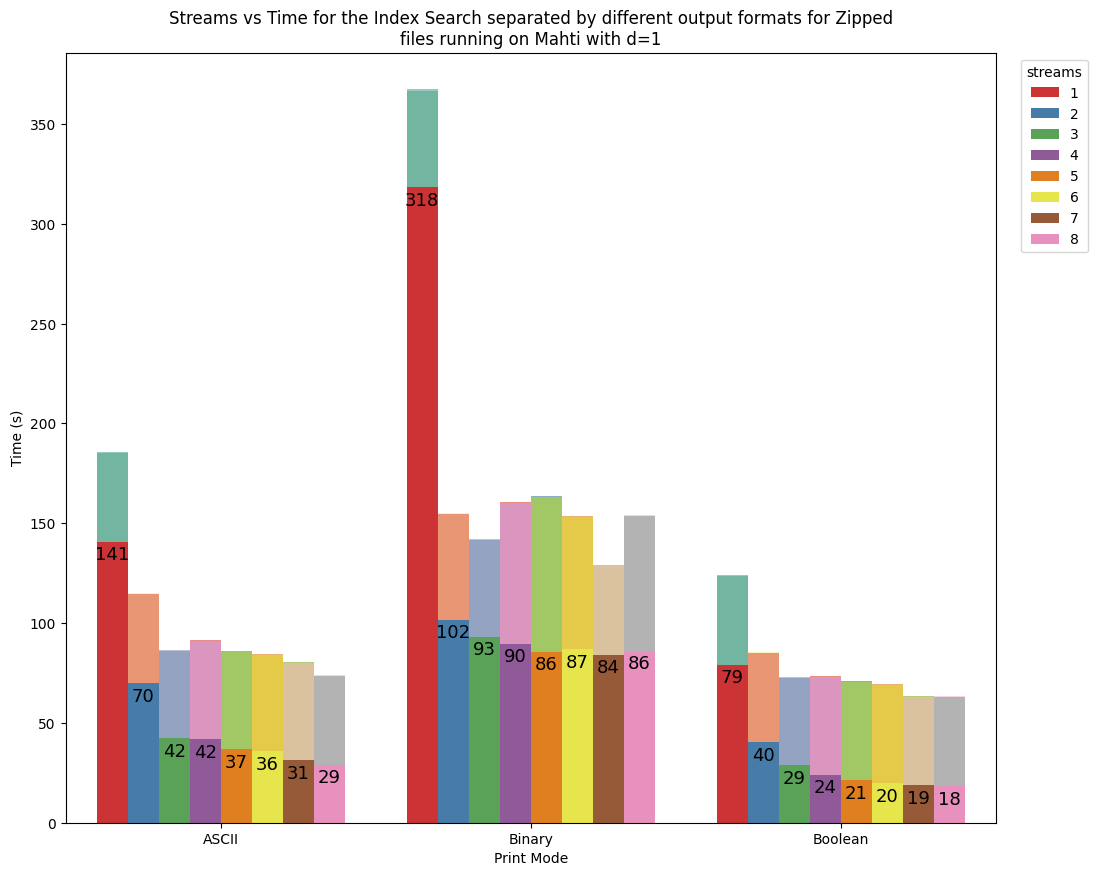
\includegraphics[width=0.7\textwidth]{images/MahtiIndexZippedD1.png}
  \caption{Timings for the Index Search with zipped inputs and $d=1$ on Mahti.}\label{fig:MahtiIndexZippedD1}
\end{figure}

\begin{figure}[t]
  \centering
  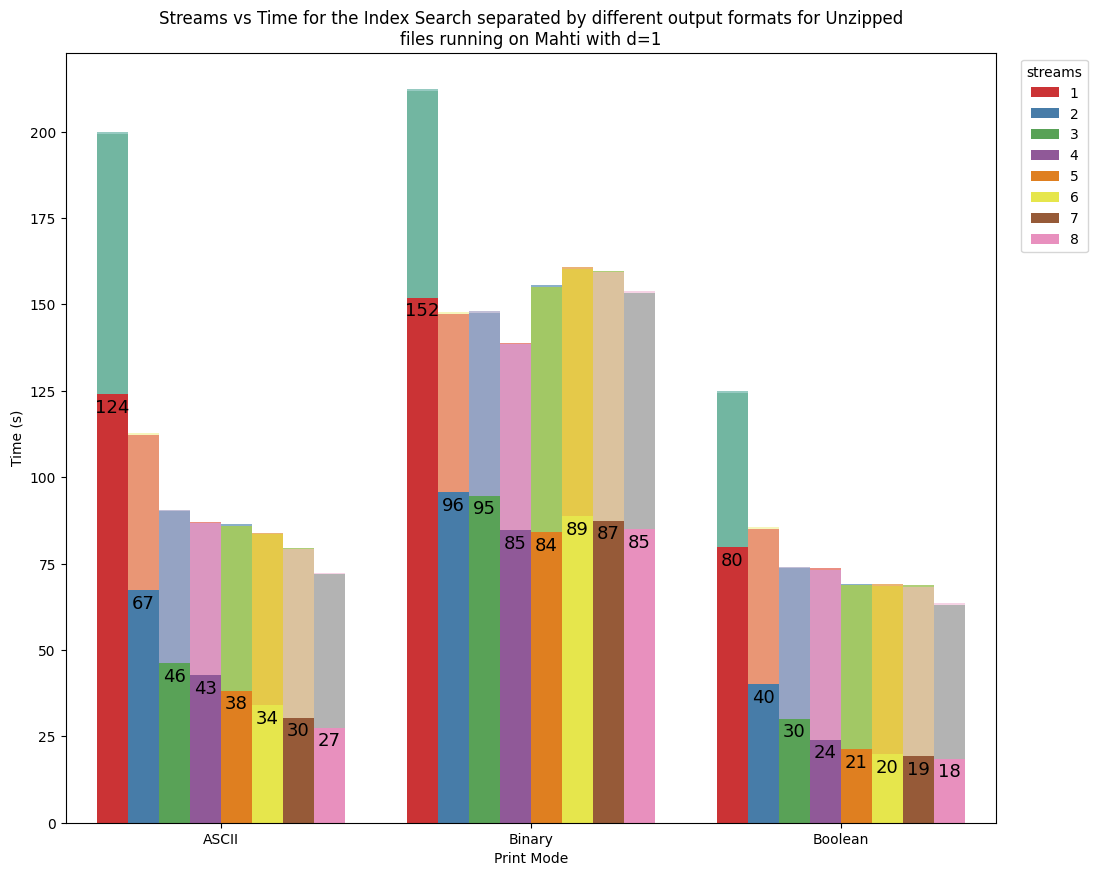
\includegraphics[width=0.7\textwidth]{images/MahtiIndexUnzippedD1.png}
  \caption{Timings for the Index Search with unzipped inputs and $d=1$ on Mahti.}\label{fig:MahtiIndexUnzippedD1}
\end{figure}

\begin{figure}[t]
  \centering
  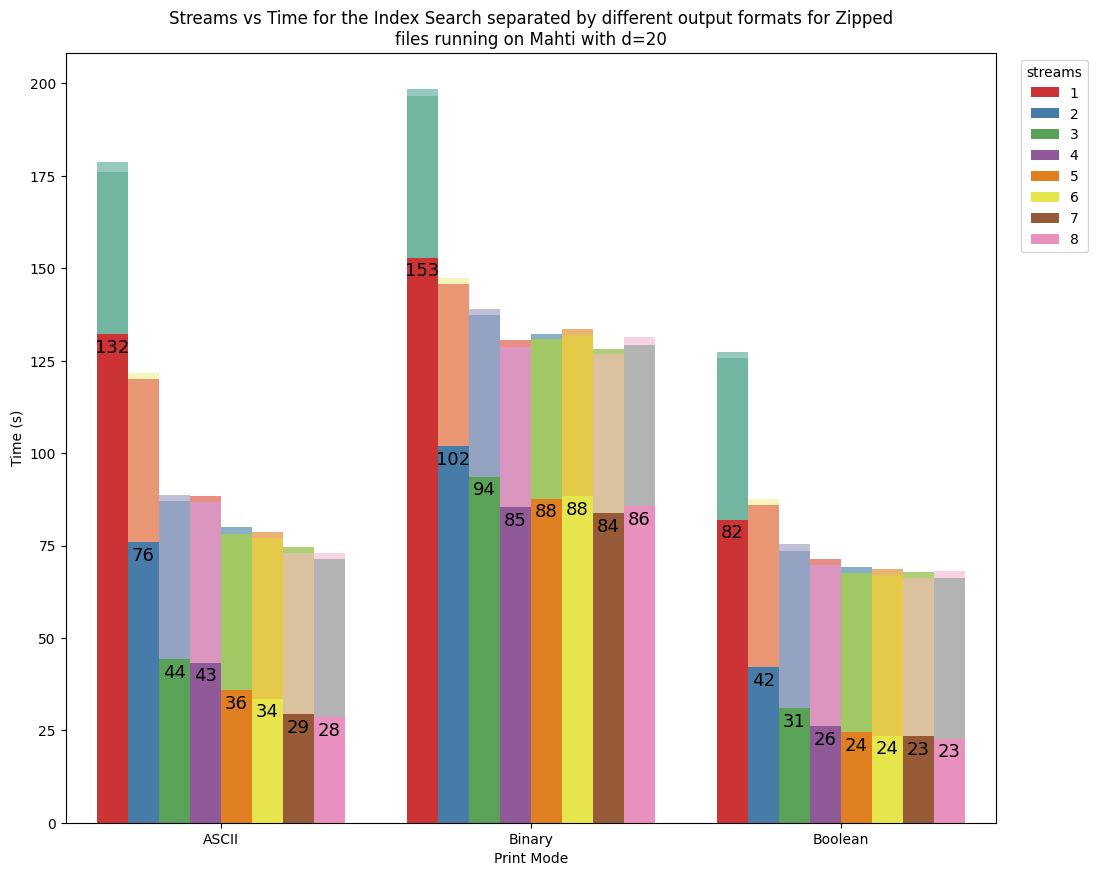
\includegraphics[width=0.7\textwidth]{images/MahtiIndexZippedD20.png}
  \caption{Timings for the Index Search with zipped inputs and $d=20$ on Mahti.}\label{fig:MahtiIndexZippedD20}
\end{figure}

\begin{figure}[t]
  \centering
  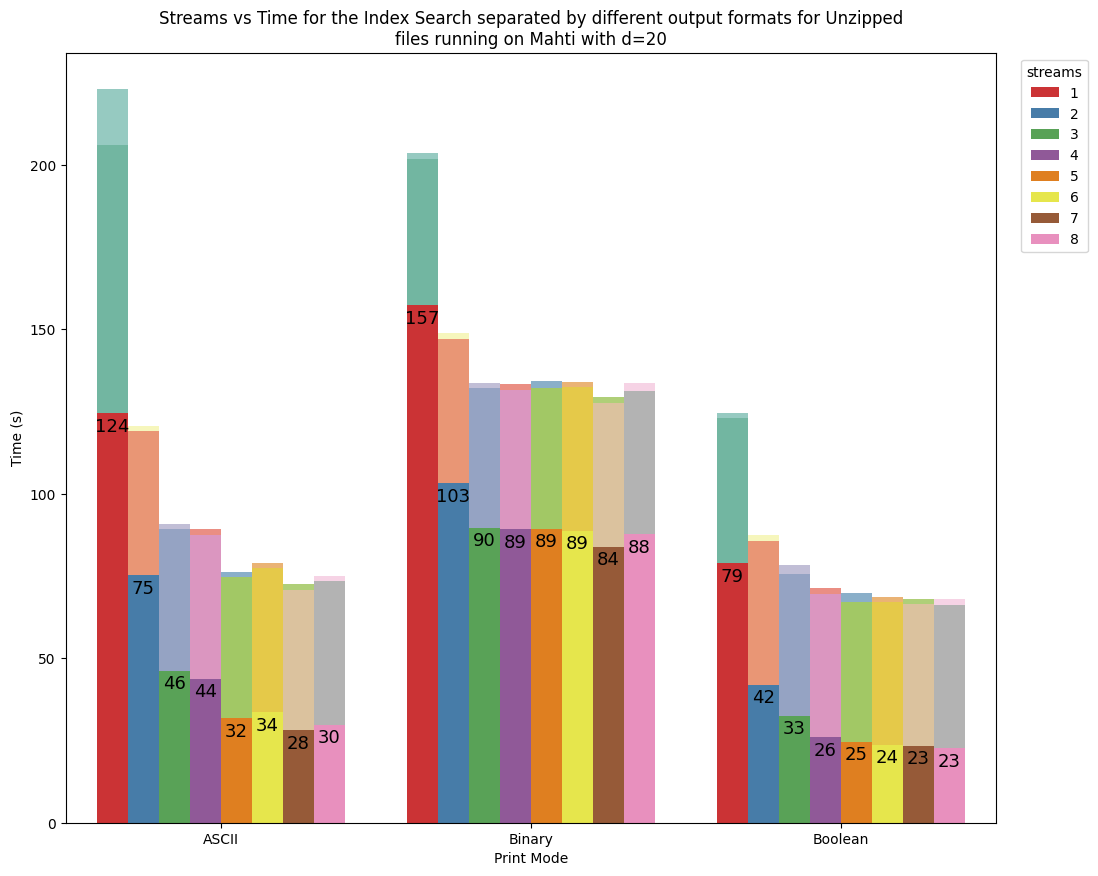
\includegraphics[width=0.7\textwidth]{images/MahtiIndexUnzippedD20.png}
  \caption{Timings for the Index Search with unzipped inputs and $d=20$ on Mahti.}\label{fig:MahtiIndexUnzippedD20}
\end{figure}

The main result format which will be focused on from the Index Search will be the ASCII format.
The reason for this is that it is the format that produces the least output, while being the fastest format which is also suitable for pseudoalignment.
It can be seen that when a single stream is considered, the I/O causes a large bottleneck since neither GPU I/O nor disk I/O is being parallelised.
The choice of the checkpoint parameter $d$ does not make much of a difference, even though the GPU kernel does more work.
This indicates that the kernel for searching is not the bottleneck.
There is also no significant difference between using the zipped or unzipped input format.

Stemming from these results, more focus will now be given to the results with the unzipped input with $d=20$.
The reasons are that the unzipped input was also given to Themisto, and the index with $d=20$ is also more scalable since the color set uses less space.
When using eight streams, the time taken to perform the search is 30 seconds, which is a throughput of 1.675 GB/s.
Figure~\ref{fig:MahtiIndexUnzippedD20S8ASCII} shows the timeline and a statistics table for this run.
One can see that most components run in parallel to each other, and even the same component type in different streams tend to run in parallel.
If the attention is then turned to the table in the same figure, whose description for each of its components can be found in Appendix~\ref{app:IndexTableDescriptions}, one may then infer that the most expensive phases are the parser which reads the files to disk, and the printer which outputs the results to disk.
This is seen in the \textit{max\_stream\_time} column, since the \textit{total\_time} column comprises the time taken by all the streams, even when they were working in parallel.
Focusing then on Figure~\ref{fig:MahtiIndexUnzippedD20S1ASCII}, which is the figure with a single stream, the reader may see the same trend, further enforcing earlier claims.

\begin{figure}[t]
  \centering
  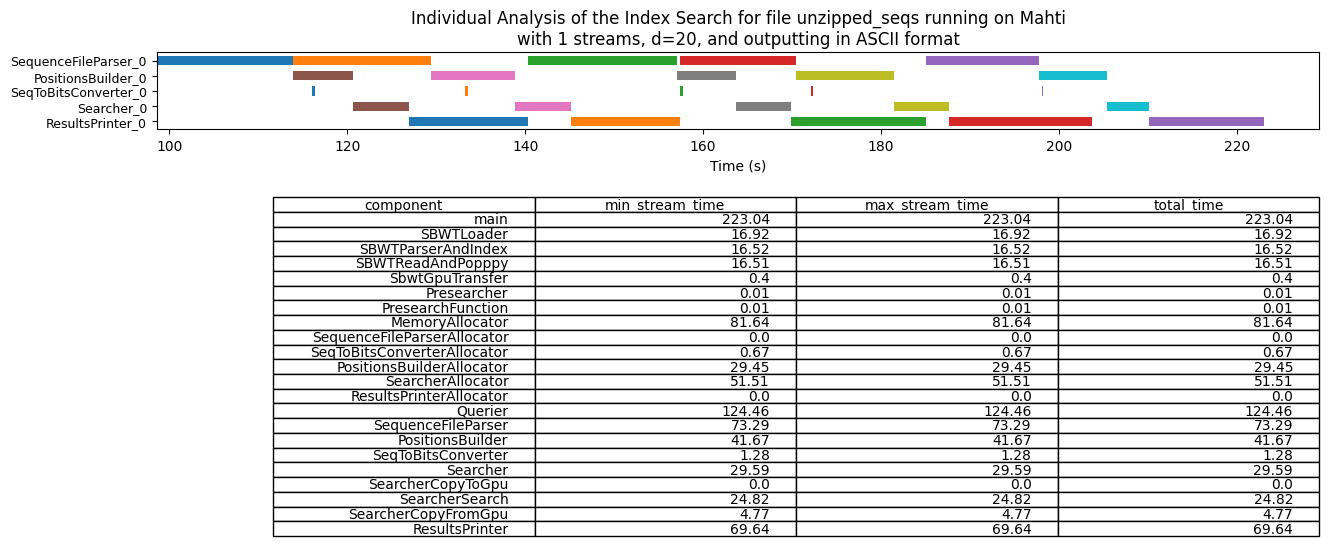
\includegraphics[width=\textwidth]{images/MahtiIndexUnzippedD20S1ASCII.png}
  \caption{Timeline for the Index Search running on Mahti with unzipped sequences as inputs, producing the ASCII format with $d=20$ and 1 streams, excluding loading and memory allocation.}\label{fig:MahtiIndexUnzippedD20S1ASCII}
\end{figure}

\begin{figure}[t]
  \centering
  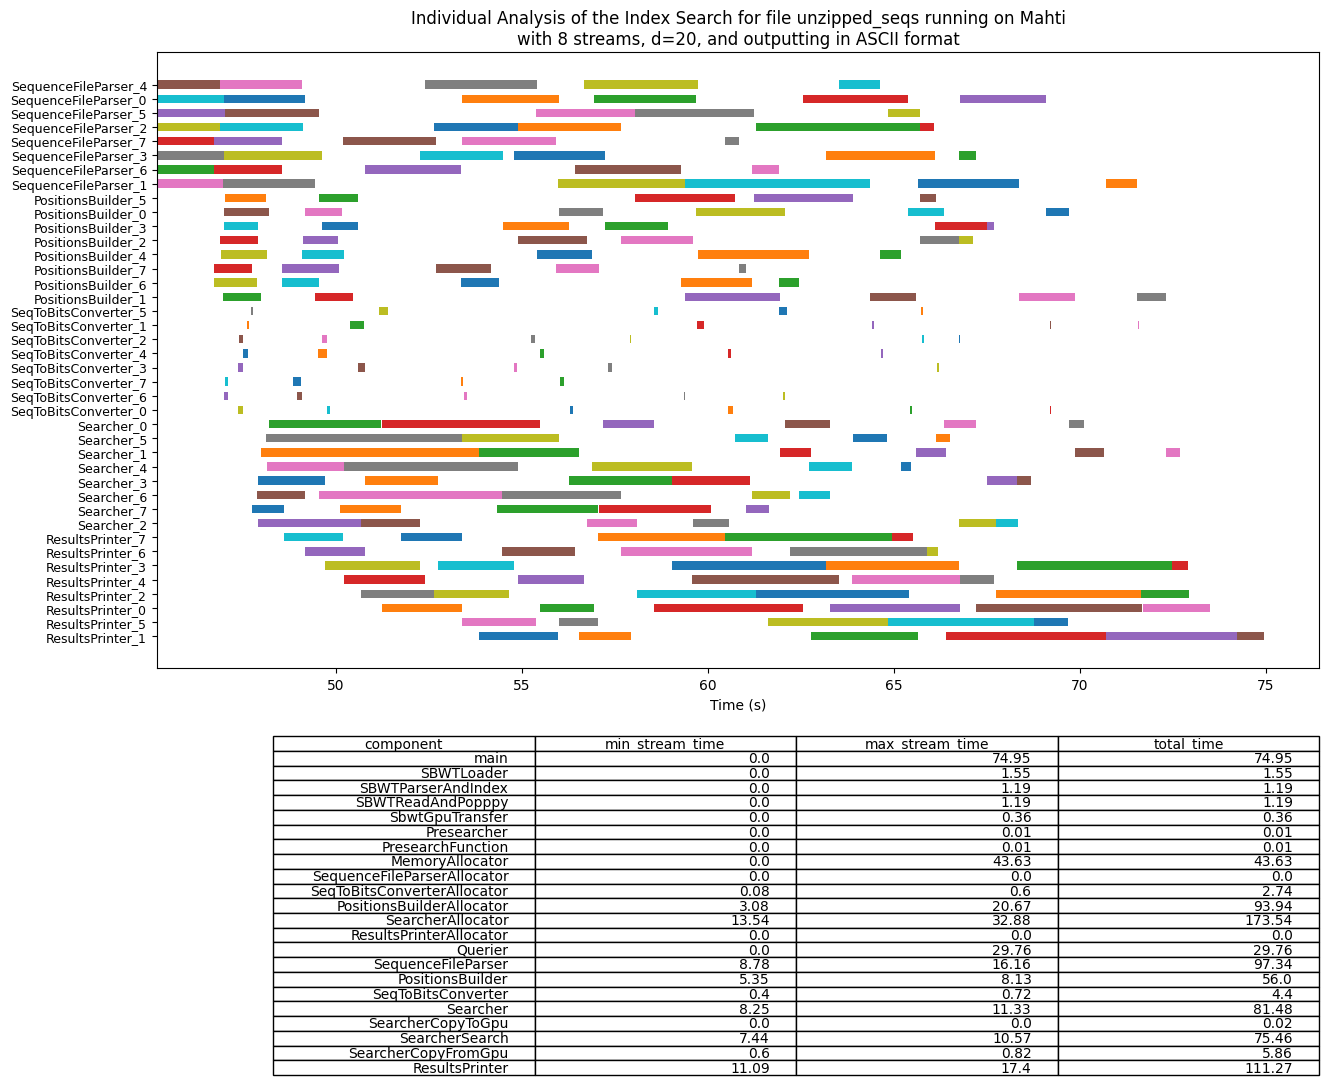
\includegraphics[width=\textwidth]{images/MahtiIndexUnzippedD20S8ASCII.png}
  \caption{Timeline for the Index Search running on Mahti with unzipped sequences as inputs, producing the ASCII format with $d=20$ and 8 streams, excluding loading and memory allocation.}\label{fig:MahtiIndexUnzippedD20S8ASCII}
\end{figure}

\subsection{LUMI}

On LUMI the story is a little different.
Note that, from now on, only the results with $d=20$ will be shown, as the results with $d=1$ are not scalable to larger indexes and the throughput is not significantly different.
In that same vein, only the unzipped sequences will be shown since these are the files whose size on which throughput is calculated on.
The first noticeable difference in Figure~\ref{fig:LumiIndexUnzippedD20} is that LUMI takes longer to process the results.
An anomaly consistently shows up for the index search with the boolean format, where the single stream outperforms multi-stream processing.
This seems to be coming from the kernel search function, which takes a much longer time as the number of streams increases.
However, the CPU processing then benefits from this as there is also multithreading there.
This may be observed from Figures~\ref{fig:LumiIndexUnzippedD20S1Boolean} and~\ref{fig:LumiIndexUnzippedD20S8Boolean}, which show the results with one and eight streams respectively.

\begin{figure}[t]
  \centering
  \includegraphics[width=0.7\textwidth]{images/LumiIndexUnzippedD20.png}
  \caption{Timings for the Index Search with unzipped inputs and d=20 on LUMI.}\label{fig:LumiIndexUnzippedD20}
\end{figure}


The results obtained for the ASCII format show a similar trend, as seen in Figures\ref{fig:LumiIndexUnzippedD20S1ASCII}  and~\ref{fig:LumiIndexUnzippedD20S8ASCII}.
As the number of streams increases, the longer the GPU kernels take.
However, since the CPU and I/O multithreading benefit from using multiple streams,
The reason for this difference, where the GPU kernel time is proportional to the streams is generally unknown, and will need to be further explored in future work beyond this thesis.
However, some possible reasons may be due to the AMD device doing fewer optimisations to the GPU kernel, or it is more susceptible to thread divergence, or the AMD device handles GPU random memory accesses worse than NVIDIA.
On LUMI, the average time taken for this index search when the number of streams is high enough, is around 120 seconds, which indicates a throughput of 418.9 MB/s.

\begin{figure}[t]
  \centering
  \includegraphics[width=\textwidth]{images/LumiIndexUnzippedD20S1Boolean.png}
  \caption{Timeline for the Index Search running on LUMI with unzipped sequences as inputs, producing the boolean format with $d=20$ and 1 streams, excluding loading and memory allocation.}\label{fig:LumiIndexUnzippedD20S1Boolean}
\end{figure}

\begin{figure}[t]
  \centering
  \includegraphics[width=\textwidth]{images/LumiIndexUnzippedD20S8Boolean.png}
  \caption{Timeline for the Index Search running on LUMI with unzipped sequences as inputs, producing the boolean format with $d=20$ and 8 streams, excluding loading and memory allocation.}\label{fig:LumiIndexUnzippedD20S8Boolean}
\end{figure}

\begin{figure}[t]
  \centering
  \includegraphics[width=\textwidth]{images/LumiIndexUnzippedD20S1ASCII.png}
  \caption{Timeline for the Index Search running on LUMI with unzipped sequences as inputs, producing the ASCII format with $d=20$ and 1 streams, excluding loading and memory allocation.}\label{fig:LumiIndexUnzippedD20S1ASCII}
\end{figure}

\begin{figure}[t]
  \centering
  \includegraphics[width=\textwidth]{images/LumiIndexUnzippedD20S8ASCII.png}
  \caption{Timeline for the Index Search running on LUMI with unzipped sequences as inputs, producing the ASCII format with $d=20$ and 8 streams, excluding loading and memory allocation.}\label{fig:LumiIndexUnzippedD20S8ASCII}
\end{figure}

\section{Color Search}

The next set of results arise from the second phase of pseudoalignment, which is the Color Search.
For this phase, the user may choose to read from the ASCII or the binary output of the first phase.
The results for $d=1$ and $d=20$ will be approximately the same, since the same work needs to be done in this phase, hence focus will be shifted towards $d=20$.
The size of the resulting ASCII and binary formats are 110 GB and 180 GB respectively.
Regarding the CSV format, this leads to files that are too large, so no results will be given for this format.
This format is only recommended for extremely dense outputs.

\subsection{Mahti}

When looking at Figure~\ref{fig:MahtiColorASCIID20}, one can, first of all, see a large difference between one stream and two.
The graph shows a decaying exponential decrease in the time taken, as more streams are added, going down to less than 70 seconds at seven and eight streams when it comes to the ASCII output format, when not considering startup.
Based on the result from the indexes, which was 49 GB, this means that this part has a throughput of 49 GB / 70s = 700 MB/s.
Meanwhile, from the FASTQ files, the total throughput of our method is $50.265$ / (30 + 70)s $\approx$ 500 MB/s, which is 17.5x faster than the best result from Themisto on the same 32 cores, or 10x times faster than when Themisto is run on 64 cores on LUMI.
The ASCII format is again much faster than the boolean format as it needs to perform less disk I/O.
To gain insight on the performance bottlenecks in this case, Figure~\ref{fig:MahtiColorASCIID20S8ASCII} shows the run with the ASCII output with eight streams.
The I/O, especially output, is the biggest bottleneck.
Copying the results from GPU to CPU memory also takes quite a long time, while the rest of the components are almost insignificant in comparison to the mentioned parts.

\begin{figure}[t]
  \centering
  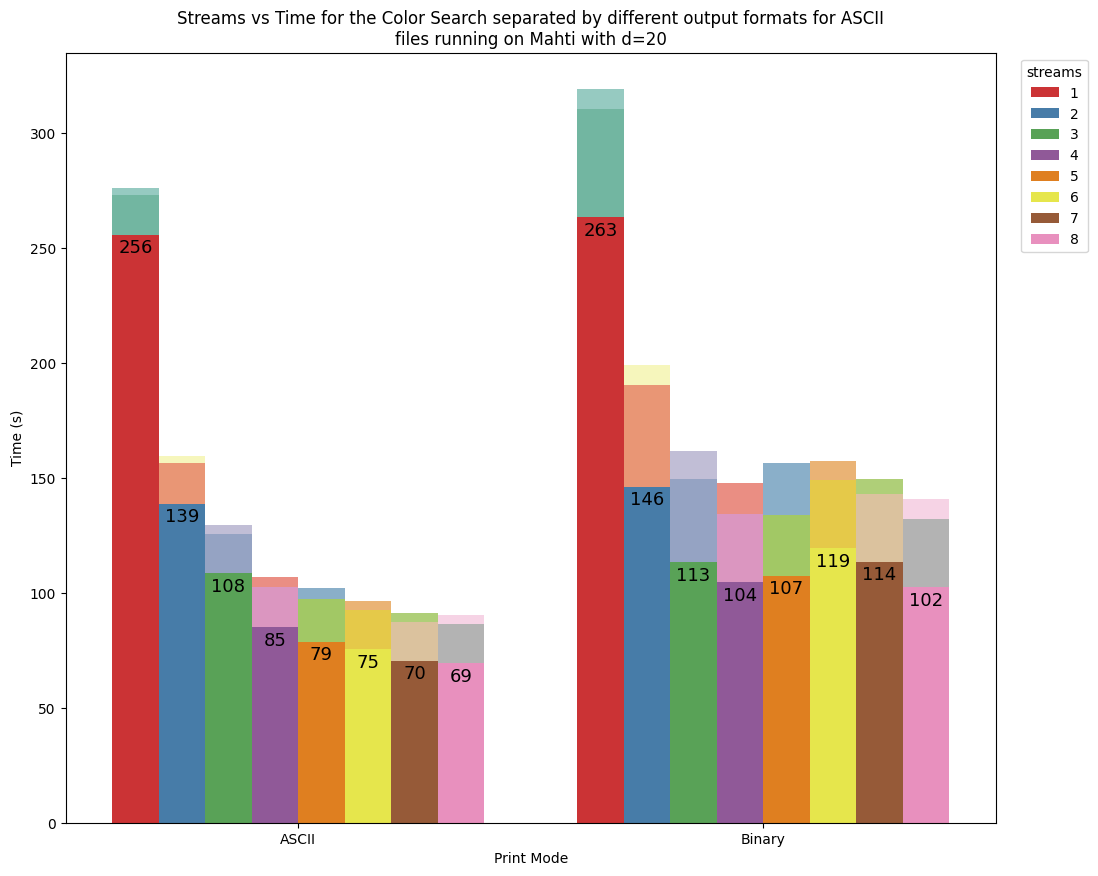
\includegraphics[width=0.7\textwidth]{images/MahtiColorASCIID20.png}
  \caption{Timing results for the Color Search, reading from the ASCII indexes, with $d=20$ running on Mahti}\label{fig:MahtiColorASCIID20}
\end{figure}

\begin{figure}[t]
  \centering
  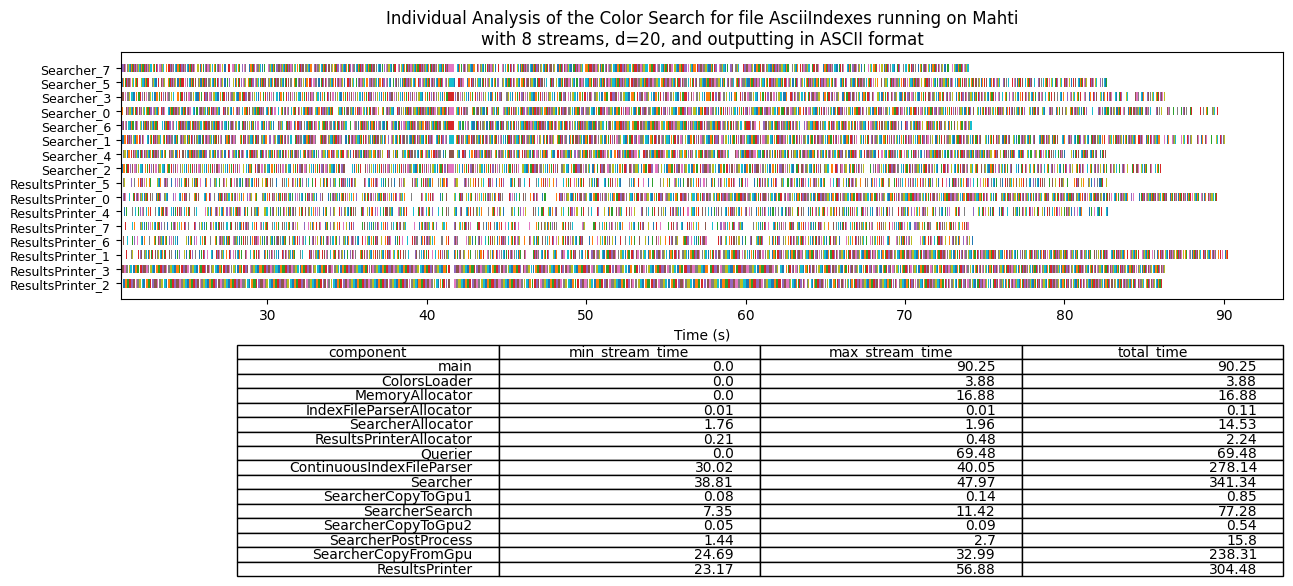
\includegraphics[width=\textwidth]{images/MahtiColorASCIID20S8ASCII.png}
  \caption{Timeline for the Color Search running on Mahti with ASCII indexes as inputs, producing the ASCII format with $d=20$ and 8 streams, excluding loading and memory allocation.}\label{fig:MahtiColorASCIID20S8ASCII}
\end{figure}

\subsection{LUMI}

Similar to the Index Search, the Color Search on LUMI is faster on the CPU side of things, but significantly slower on the GPU.
Figure~\ref{fig:LumiColorASCIID20} shows the overall results of the Color Search when reading from the ASCII indexes.
This time, there is less difference between using a single stream or multiple streams.
The results are also less consistent, with a remaining uncertainty in why this is the case.
With Figure~\ref{fig:LumiColorASCIID20S8ASCII}, which shows the run with eight streams, one may see that most time is taken with the searching part of this phase.
Everything else is faster than when run on Mahti with a moderate margin.

\begin{figure}[t]
  \centering
  \includegraphics[width=0.7\textwidth]{images/LumiColorASCIID20.png}
  \caption{Timing results for the Color Search, reading from the ASCII indexes, with $d=20$ running on LUMI}\label{fig:LumiColorASCIID20}
\end{figure}

\begin{figure}[t]
  \centering
  \includegraphics[width=\textwidth]{images/LumiColorASCIID20S8ASCII.png}
  \caption{Timeline for the Color Search running on LUMI with ASCII indexes as inputs, producing the ASCII format with $d=20$ and 8 streams, excluding loading and memory allocation.}\label{fig:LumiColorASCIID20S8ASCII}
\end{figure}

With an average time taken of 450s, when considering that the indexes read are 49 GB, this phase has a throughput of 109 MB/s.
If the entire pipeline is considered, with the FASTQ inputs of $50.265$ GB, then the end-to-end throughput is $50.265$ / (120s + 450s) $\approx$ 88MB/s, which is 70\% faster than Themisto.
Thus, even though the GPU kernel is much slower than on Mahti, the gains are still substantial enough to consider using, given a large enough dataset.

\chapter{Conclusion}\label{ch:Conclusion}

Thus this thesis comes to a conclusion.
A highly parallelised implementation of Themisto was presented which uses all available computational resources.
The background which preceded this thesis was thoroughly presented alongside all the biological and algorithmic research.
The full method including the several modes of parallelisation used was then discussed in Chapter~\ref{ch:Methodology}.
The results were then discussed in Chapter~\ref{ch:Results}, with a detailed discussion and reasons for why certain results are the way there are were given, with uncertainties pointed out and left for future work.

With regard to the research questions, the CPU side has been improved through using parallel disk I/O and using a multithreaded pipeline.
Since sequences can be divided into parts, different threads will get an equal amount of work, by getting the same amount of characters or indexes to process.
Then, the GPU implementation has been improved by allowing $k \ge 32$ through a small change in the GPU kernel, which did not significantly impact performance.
Furthermore, the algorithm presented in this thesis can differentiate between $k$-mers which are invalid and those not found in the graph by using a simple boolean list and some changes in the printing of results.
Lastly, the color search was put on the GPU and when comparing the best version to the best version of Themisto, the GPU is 10 times faster than this.
The final section of this thesis will discuss how this research may be extended and improved.

\section{Future Work}

In terms of extending the work done in this thesis, there are several which may be made, each providing different contributions.
One more optimisation which can be made is to attempt using unified memory\footnote{\url{https://developer.nvidia.com/blog/unified-memory-cuda-beginners/}} for possibly better GPU memory transfers.
Additionally, when $\tau=1$ in phase two, it would be enough to represent each color count with a single bit, that is, if it appears or not, and then using a bitwise $AND$ to intersect the colors.
As stated before, this optimisation is already done by Kallisto and Themisto.
In terms of new features, the ability to write in a compressed format would make the method even more usable by more institutions.
Moreover, an implementation where the GPU components are put on the CPU, while keeping all the parallelisations introduced in this thesis, would be an interesting comparison, to see how far a CPU implementation can be taken.
It was also stated in Subsection~\ref{subs:ColorSearch} that the method used in this thesis wastes a lot of memory if most color counts are zeros, so a new implementation that overcomes this hurdle may also significantly improve throughput.

Further results using this method could also be obtained by analysing how it scales with different datasets, compared to the CPU version.
Different values of $k$ may also lead to different results.
Another way to evaluate the results would be to use them for pseudoaligning an existing dataset and test how taking the invalid characters into account affects the accuracy of pseudoalignment.
A deeper analysis may also be made into each of the components, such as analysing why runs on LUMI take so long in the GPU when compared to Mahti.
Lastly, with the introduction of Fulgor, it would be interesting to see its methods executed on the GPU alongside the parallelisations presented both here and in their work.


\cleardoublepage %fixes the position of bibliography in bookmarks
\phantomsection

\addcontentsline{toc}{chapter}{\bibname} % This lines adds the bibliography to the ToC
\bibliographystyle{abbrv} % numbering alphabetic order
\bibliography{bibliography}

\chapter{Appendix}

\section{Index Search Data Structures}\label{app:IndexSearchDataStructures}

\begin{itemize}
  \item \textbf{seq}: The sequence of characters as read from the FASTA/FASTQ files. May contain any character in the ASCII list. It is basically a string of characters, that may contain items other than our four characters alphabet of $ACGT$. This may contain characters from different sequences, too. The parser keeps reading the list of files for new characters until the maximum number of characters it should read in a single batch is read, or until the maximum number of different sequences it can span is reached, or until the end of the files is reached.
  \item \textbf{chars\_before\_newline}: An array of the number of characters which must be processed before the next character is considered to originate from a new sequence. For example, given the array $[4, 10, \infty]$, then it is known that the first four characters in \textbf{seq} are from the first sequence, the next six characters are from the second sequence, whereas the rest of the characters are from the third sequence. Note that this does not mean that the first sequence is four characters long, nor does the algorithm know how long the last sequence is, since a sequence may be split between two batches, for load balancing, hence why this array is important. A part of the first sequence may have been part of the previous batch, or could have spanned more than two batches if it was super long, whereas the third sequence may have been too large to fit in this batch, so the next batch will need to process the next part of it.
  \item \textbf{newlines\_before\_newfile}: Similar to what \textbf{chars\_before\_newline} is for characters, but instead this works for sequences. Thus, given the array $[3, 4, \infty]$, it means that in the input for this batch, the sequences came from three files, and the first three sequences came from the first file, the fourth sequence came from the second file, whereas the last sequence came from the third file. Note that this does not mean that the first file is three sequences long, nor does the algorithm know how large the third file is, since a file may be split between two batches, for load balancing, hence why this array is important.
  \item \textbf{bits}: Using a full byte for each character is wasteful when the alphabet is only four characters. Thus it is possible to convert $ACGT$ to $00, 01, 10, 11$ respectively, and this array of u64s contains the bitpacked characters. Thus, a single u64 can hold 32 characters, so to hold more than 32 characters per batch, an array of u64s is used, which is what this array is used for.
  \item \textbf{invalid\_chars}: Sometimes the sequences in the FASTQ file, and therefore contents of the \textbf{seq} string, may contain characters other than $ACGT$. The $k$-mers which contain these characters are invalid for this use case, and should thus be marked as such. Therefore, this array of booleans contains the same amount of elements as \textbf{seq}, and contains a 0 if the corresponding character at the same index in \textbf{seq} is part of the $ACGT$ alphabet, otherwise it will contain 1. For example, given \textbf{seq} \textit{ACNBGT}, this array will contain $[0, 0, 1, 1, 0, 0]$, as characters $N$ and $B$ are invalid. For the implementation in this algorithm, an array of chars is used rather than booleans, as this data type was found to be slightly faster, since the CPU does not need to perform any unnecessary bit shifts.
  \item \textbf{positions}: There are fewer $k$-mers than there are characters. If there are 10 characters in a sequence and $k=7$, then there are 4 $k$-mers in this sequence, and the first character of these $k$-mers would be the characters at indexes 0, 1, 2, and 3. These indexes are the positions array. When there are multiple sequences, so if the algorithm is given two sequences, each 10 characters long, and they would be in the same batch, that is, \textbf{seq} is of size 20, then the positions array would be $[0, 1, 2, 3, 10, 11, 12, 13]$, as the $k$-mers for the second sequence start later, at index 10.
\end{itemize}

\section{Color Search Data Structures}\label{app:ColorSearchDataStructures}

\begin{itemize}
  \item \textbf{warped\_indexes}: The indexes of colored sequences in a u64 array. When the indexes are read from the file, they are put into this array, which will later be put on the GPU. The goal is such that each thread in the GPU handles a single index, and a single warp handles indexes from a single sequence. This means that a warp can not have indexes from two different sequences. However, the indexes of a sequence are allowed to be spread over multiple warps. Thus, the indexes are loaded until the end of a sequence, and then padding is inserted for the rest of the warp, so that the first index of the next sequence will be loaded at the first position of the next warp. So, given two sequences with indexes $[45, 21, 32, 25, 21]$ and $[23, 22, 93, 34]$, and given a warp size of 4, then this array would contain $[45, 21, 32, 25, 21, -1, -1, -1, 23, 22, 93, 34]$, where the $-1$ represents padding, the first eight indexes are of the first and second warp, which contain the indexes of the first sequence plus padding, and the last four indexes are of the third warp which contain the indexes of the second sequence. Since the second sequence has an index count which is a multiple of the warp size, there is no need for padding.
  \item \textbf{warp\_intervals}: The indexes are all in a single array, inside the \textbf{warped\_indexes}. Therefore, there needs to be some mechanism to tell which indexes come from the first sequence, and which indexes come from the second sequence. This array provides that mechanism, such that it tells at which warp index a new sequence starts. Given the previous example, this array would contain $0, 2, 3$. The last value exists for convenience, and it allows the programmer to know how many warps in total are loaded with indexes.
  \item \textbf{found\_idxs}: When $\tau$ is not equal to 1, it is necessary to check if enough indexes of the sequence actually belong to the DBG. This array takes a count of how many indexes of each sequence belong to the DBG. Note that a colored sequence has this value equal to at least 1. Therefore, this array has a single entry per sequence.
  \item \textbf{not\_found\_idxs}: When $\tau$ is not equal to 1, it is thus also necessary to know how many indexes of the sequence are not found in the DBG. This array takes count of those. Thus it also has one entry per sequence.
  \item \textbf{invalid\_idxs}: In the implementation provided in this thesis, a distinction is made between indexes which are not found and those which are invalid, hence this array contains a count of how many invalid indexes existed for each sequence.
  \itm \textbf{results}: This array contains the colors of the colored sequences, after they are post processed in the GPU. The format of this array takes a lot of space, such that if there are $n$ colors in total, and $m$ colored sequence, this array takes $nm$ spaces.
  \item \textbf{colored\_seq\_id}: Since not all sequences have entries in \textbf{warped\_indexes}, the algorithm needs to know where the colors of a colored sequence are after post processing. It can know if a sequence is colored or not by simply checking if the \textbf{found\_idxs} for this sequence is greater than zero. If the sequences are accessed serially, then it would be easy to know which colors belong to which sequence, simply by keeping a counter, and after encountering a colored sequence, the counter would be increased by one. However, if the results and the sequences are to be accessed in parallel, then this array allows the algorithm to know where to look for the \textbf{results} of this sequence. Thus, this array also has an entry per sequence, however, the blank sequences ignore this value as they do not have any entries in the \textbf{results} array.
  \item \textbf{seqs\_before\_newfile}: This is the same as for the Index Search phase, it keeps track of how many sequences belong to the first file, how many for the second, etc.
\end{itemize}

\section{Components and Batches}\label{app:Batches}

\begin{figure}[h!]
  \centering
  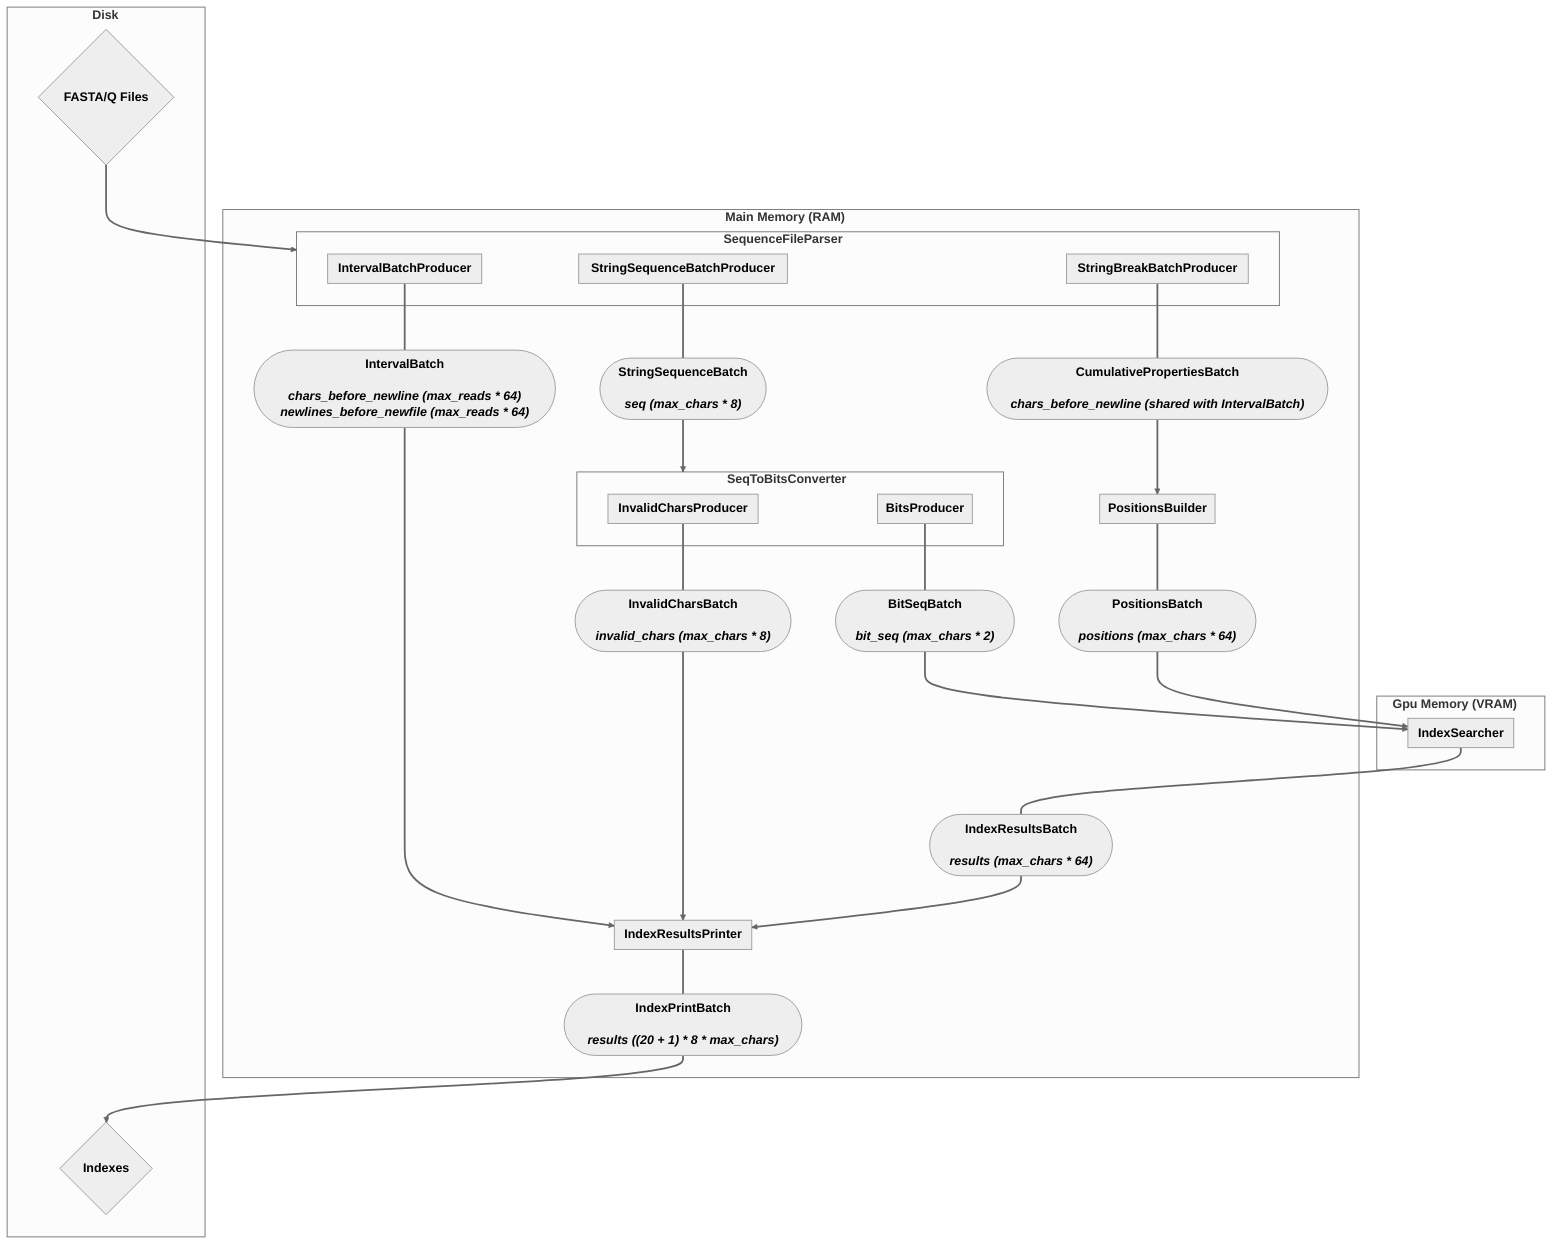
\includegraphics[width=\textwidth]{images/IndexBatches.png}
  \caption{The Index components and how their batches are shared between components. The amount of space that each batch uses is also listed below it, with the format of <variable>(<size taken>). These sizes are taken into consideration when reserving memory for each batch, by first deciding the maximum number of characters and then reserving memory accordingly. The diamond shapes represent items stored on disk, square shapes represent components, and items in the rectangle with curved sides are the batches.}\label{fig:IndexBatches}
\end{figure}


\begin{figure}[h!]
  \centering
  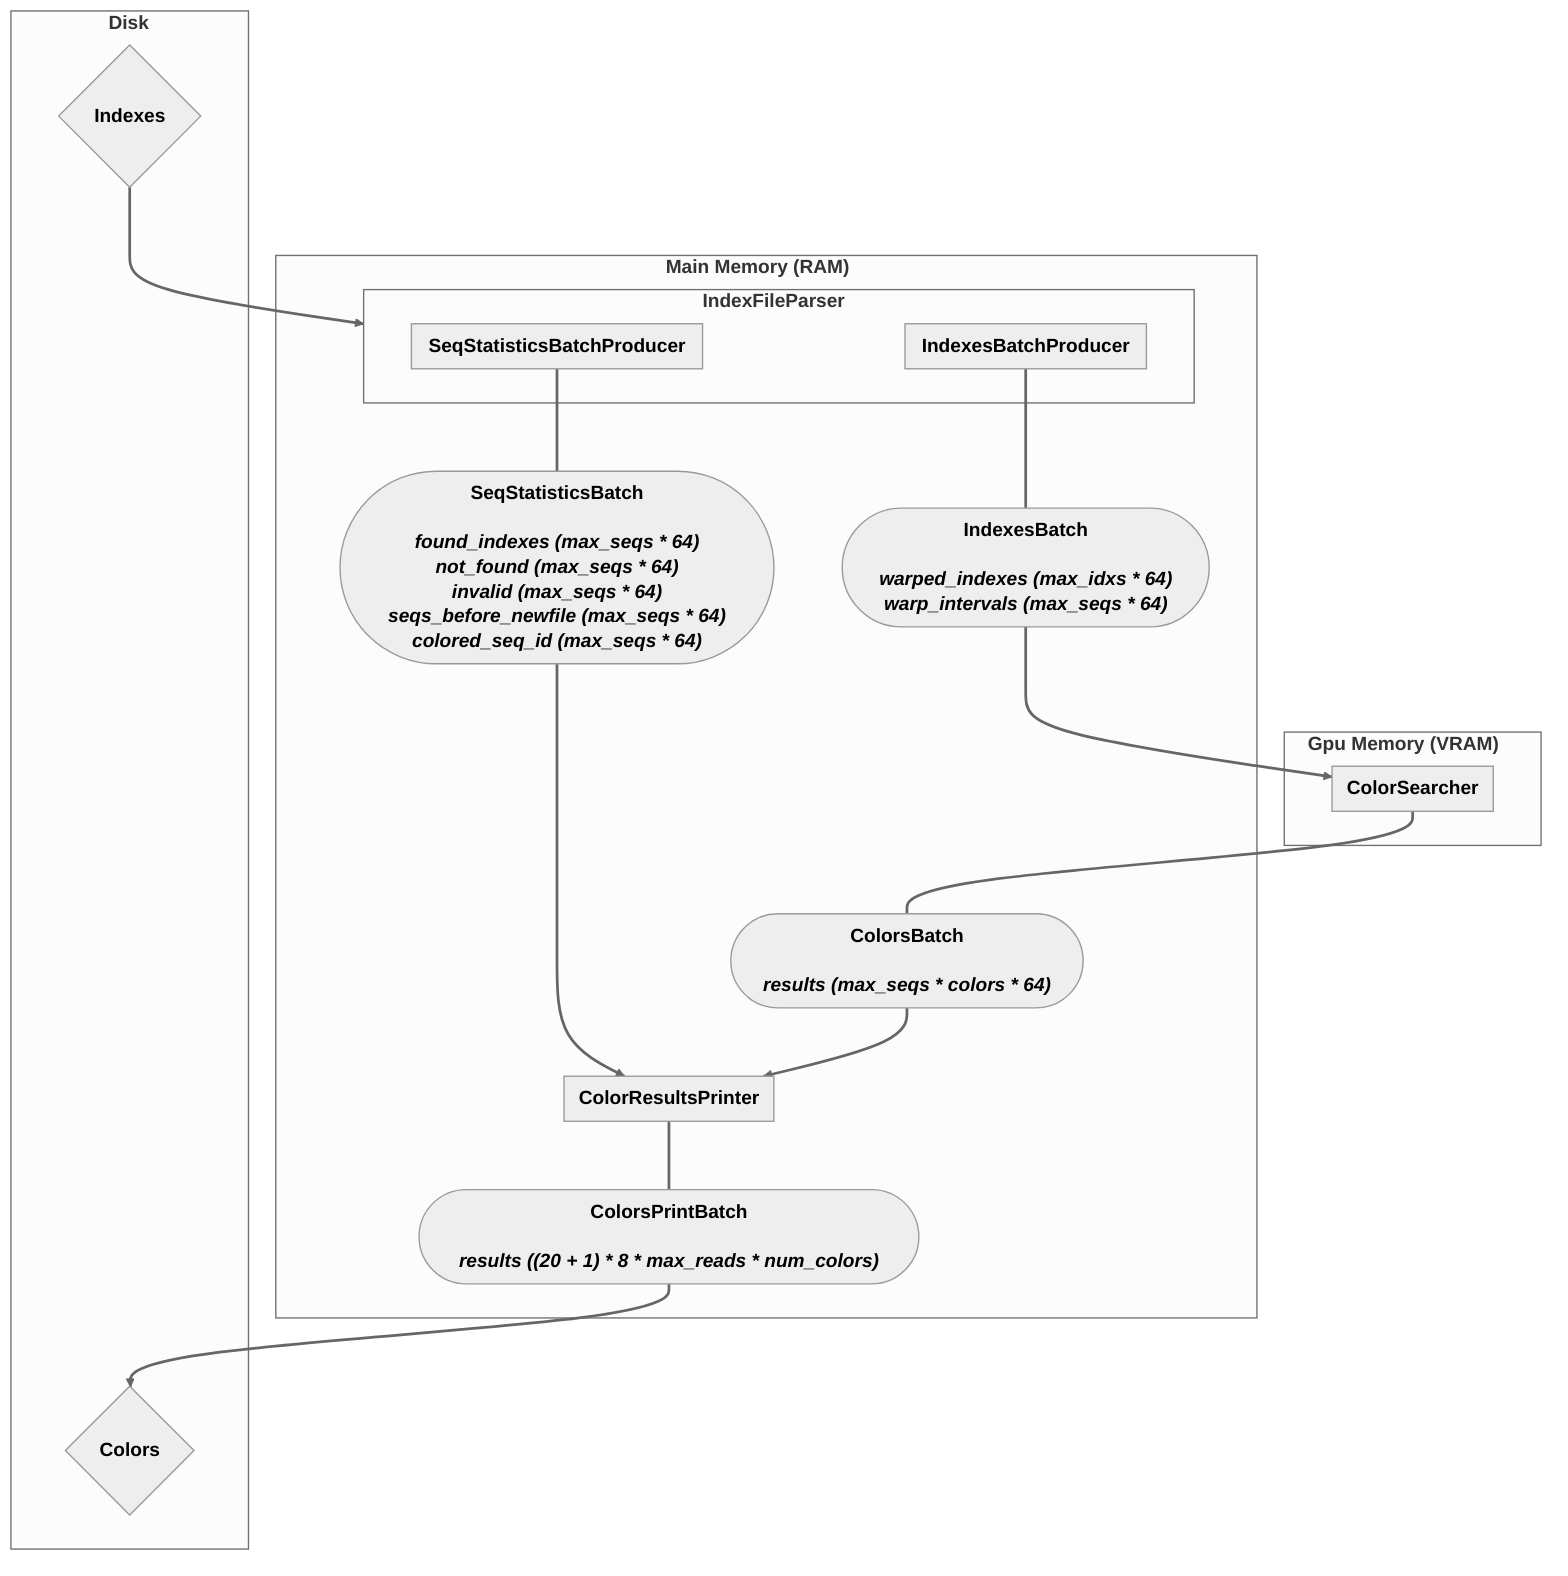
\includegraphics[width=\textwidth]{images/ColorBatches.png}
  \caption{The Colors components and how their batches are shared between components. The amount of space that each batch uses is also listed below it, with the format of <variable>(<size taken>). These sizes are taken into consideration when reserving memory for each batch, by first deciding the maximum number of characters and then reserving memory accordingly. The diamond shapes represent items stored on disk, square shapes represent components, and items in the rectangle with curved sides are the batches.}\label{fig:ColorBatches}
\end{figure}

\clearpage
\section{Dataset Filename List}\label{app:file_names}

\begin{footnotesize}
\begin{verbatim}
  ftp.sra.ebi.ac.uk/vol1/fastq/ERR340/004/ERR3404624/ERR3404624_2.fastq.gz
  ftp.sra.ebi.ac.uk/vol1/fastq/ERR340/005/ERR3404625/ERR3404625_1.fastq.gz
  ftp.sra.ebi.ac.uk/vol1/fastq/ERR340/005/ERR3404625/ERR3404625_2.fastq.gz
  ftp.sra.ebi.ac.uk/vol1/fastq/ERR340/006/ERR3404626/ERR3404626_1.fastq.gz
  ftp.sra.ebi.ac.uk/vol1/fastq/ERR340/006/ERR3404626/ERR3404626_2.fastq.gz
  ftp.sra.ebi.ac.uk/vol1/fastq/ERR340/007/ERR3404627/ERR3404627_1.fastq.gz
  ftp.sra.ebi.ac.uk/vol1/fastq/ERR340/007/ERR3404627/ERR3404627_2.fastq.gz
  ftp.sra.ebi.ac.uk/vol1/fastq/ERR340/008/ERR3404628/ERR3404628_1.fastq.gz
  ftp.sra.ebi.ac.uk/vol1/fastq/ERR340/008/ERR3404628/ERR3404628_2.fastq.gz
  ftp.sra.ebi.ac.uk/vol1/fastq/ERR340/009/ERR3404629/ERR3404629_1.fastq.gz
  ftp.sra.ebi.ac.uk/vol1/fastq/ERR340/009/ERR3404629/ERR3404629_2.fastq.gz
  ftp.sra.ebi.ac.uk/vol1/fastq/ERR340/000/ERR3404630/ERR3404630_1.fastq.gz
  ftp.sra.ebi.ac.uk/vol1/fastq/ERR340/000/ERR3404630/ERR3404630_2.fastq.gz
  ftp.sra.ebi.ac.uk/vol1/fastq/ERR340/001/ERR3404631/ERR3404631_1.fastq.gz
  ftp.sra.ebi.ac.uk/vol1/fastq/ERR340/001/ERR3404631/ERR3404631_2.fastq.gz
  ftp.sra.ebi.ac.uk/vol1/fastq/ERR340/002/ERR3404632/ERR3404632_1.fastq.gz
  ftp.sra.ebi.ac.uk/vol1/fastq/ERR340/002/ERR3404632/ERR3404632_2.fastq.gz
  ftp.sra.ebi.ac.uk/vol1/fastq/ERR340/003/ERR3404633/ERR3404633_1.fastq.gz
  ftp.sra.ebi.ac.uk/vol1/fastq/ERR340/003/ERR3404633/ERR3404633_2.fastq.gz
  ftp.sra.ebi.ac.uk/vol1/fastq/ERR340/004/ERR3404634/ERR3404634_1.fastq.gz
  ftp.sra.ebi.ac.uk/vol1/fastq/ERR340/004/ERR3404634/ERR3404634_2.fastq.gz
  ftp.sra.ebi.ac.uk/vol1/fastq/ERR340/005/ERR3404635/ERR3404635_1.fastq.gz
  ftp.sra.ebi.ac.uk/vol1/fastq/ERR340/005/ERR3404635/ERR3404635_2.fastq.gz
  ftp.sra.ebi.ac.uk/vol1/fastq/ERR340/006/ERR3404636/ERR3404636_1.fastq.gz
\end{verbatim}
\end{footnotesize}

\clearpage
\section{Results Table Description}

In Chapter~\ref{ch:Results}, there are figures with timelines and a table underneath the timeline.
These bullet points give a description of what each component means.
When a bullet point is a sub-bullet of another item, it means that the parent item includes the time of the sub-bullet.

\subsubsection{Index Search}\label{app:IndexTableDescriptions}

\begin{itemize}
  \item \textbf{main}: The entire program from start to finish.
  \begin{itemize}
    \item \textbf{SBWTLoader}: The starting phase besides memory loading.
    \begin{itemize}
      \item \textbf{SBWTParserAndIndex}: Reading the SBWT from disk, building the poppy, and transferring to GPU.
      \begin{itemize}
        \item \textbf{SBWTReadAndPoppy}: Same as parent but without the construction of the class which does the work.
      \end{itemize}
      \item \textbf{SBWTGpuTransfer}: Copying the SBWT to GPU.
      \item \textbf{Presearcher}: The construction of the presearch map.
      \begin{itemize}
        \item \textbf{PresearchFunction}: Same as parent but without construction of objects such as the allocation in GPU memory.
      \end{itemize}
    \end{itemize}
    \item \textbf{MemoryAllocator}: The allocation of memory for each of the components, some of which is pinned memory.
    \begin{itemize}
      \item \textbf{SequenceFileParserAllocator}: Memory allocation for the SequenceFileParser.
      \item \textbf{SeqToBitsConverterAllocator}: Memory allocation for the SeqToBitsConverter.
      \item \textbf{PositionsBuilderAllocator}: Memory allocation for the PositionsBuilder.
      \item \textbf{SearcherAllocator}: Memory allocation for the Searcher, on both CPU and GPU.
      \item \textbf{ResultsPrinterAllocator}: Memory allocation for the ResultsPrinter.
    \end{itemize}
    \item \textbf{Querier}: The query time, which is the time taken by the program without the startup.
    \begin{itemize}
      \item \textbf{SequenceFileParser}: The component which reads the sequence FASTA or FASTQ files.
      \item \textbf{PositionsBuilder}: The component which builds the positions.
      \item \textbf{SeqToBitsConverter}: The component which bit-packs sequences.
      \item \textbf{Searcher}: The component which searches for the indexes given the necessary items on the GPU.
      \begin{itemize}
        \item \textbf{SearcherCopyToGpu}: Copying the positions and bit-packed sequences to GPU.
        \item \textbf{SearcherSearch}: The kernel itself.
        \item \textbf{SearcherCopyFromGpu}: Copying the results back to CPU.
      \end{itemize}
    \end{itemize}
    \item \textbf{ResultsPrinter}: Printing the results to disk.
  \end{itemize}
\end{itemize}

\subsubsection{Color Search}

\begin{itemize}
  \item \textbf{main}: The entire program from start to finish.
  \begin{itemize}
    \item \textbf{ColorsLoader}: Reading the colors from disk and into the GPU.
    \item \textbf{MemoryAllocator}: The allocation of memory for each of the components, some of which is pinned memory.
    \begin{itemize}
      \item \textbf{IndexFileParserAllocator}: Memory allocation for the IndexFileParser.
      \item \textbf{SearcherAllocator}: Memory allocation for the Searcher, on both CPU and GPU.
      \item \textbf{ResultsPrinterAllocator}: Memory allocation for the ResultsPrinter.
    \end{itemize}
    \item \textbf{Querier}: The query time, which is the time taken by the program without the startup.
    \begin{itemize}
      \item \textbf{ContinuousIndexFileParser}: The component which reads the index files.
      \item \textbf{Searcher}: The component which searches for the colors and does post processing, given the necessary items on the GPU.
      \begin{itemize}
        \item \textbf{SearcherCopyToGpu1}: Copying the indexes to GPU.
        \item \textbf{SearcherSearch}: The kernel for searching.
        \item \textbf{SearcherCopyToGpu2}: Copying the warps intervals to GPU.
        \item \textbf{SearcherPostProcess}: The kernel for post processing.
        \item \textbf{SearcherCopyFromGpu}: Copying the results back to CPU.
      \end{itemize}
    \item \textbf{ResultsPrinter}: Printing the results to disk.
    \end{itemize}
  \end{itemize}
\end{itemize}


\end{document}
